% =====================================================================
%  var-task-rep -- Minimal proposal skeleton
%  One grey box per section. Add \subsection{...} freely inside any
%  section; each new subsection can carry its own box: \ph{ID}{title}{notes}.
% =====================================================================
\documentclass[11pt,a4paper]{article}

\usepackage[utf8]{inputenc}
\usepackage[T1]{fontenc}
\usepackage[margin=2.5cm]{geometry}
\usepackage{amsmath,amssymb,amsthm}
\usepackage{booktabs}
\usepackage{array}
\usepackage{longtable}
\usepackage{graphicx}
\usepackage{float}
\usepackage{fvextra}
\DefineVerbatimEnvironment{promptbox}{Verbatim}{breaklines,breakanywhere,fontsize=\footnotesize,frame=single,framesep=2mm}
\usepackage{xcolor}
\usepackage[most]{tcolorbox}
\usepackage[round,authoryear]{natbib}
\usepackage[colorlinks=true,linkcolor=blue!50!black,citecolor=green!40!black,urlcolor=blue!60!black]{hyperref}

% Placeholder box: \ph{ID}{What goes here}{Notes}
\definecolor{phframe}{gray}{0.55}
\definecolor{phback}{gray}{0.95}
\newcommand{\ph}[3]{%
  \hypertarget{ph:#1}{}%
  \begin{tcolorbox}[enhanced,breakable,colback=phback,colframe=phframe,
    boxrule=0.4pt,arc=1mm,left=2mm,right=2mm,top=1mm,bottom=1mm,
    fonttitle=\sffamily\small\bfseries,coltitle=black,colbacktitle=gray!25,
    title={[#1]\quad TO WRITE --- #2}]
  \small #3
  \end{tcolorbox}}

% Inline value to be decided
\newcommand{\tbd}[1]{\textcolor{red!70!black}{\textsf{[TBD: #1]}}}

% Link back to the status table, placed under each section heading
\newcommand{\backtostatus}{\noindent{\hfill\footnotesize\hyperref[sec:status]{$\uparrow$\,status}}\par}

% Status row: \strow{label}{name}{content}{status}
\newcommand{\strow}[4]{\hyperref[#1]{#2} & #3 & #4 \\}

\newtheorem{definition}{Definition}
\newtheorem{hypothesis}{Hypothesis}

\title{Lexical Task Heads: Identifying Them on Simple Tasks\\ with Logit Lens and Jacobian Lens Readouts}
\author{Filippo Merlo}
\date{Draft --- \today}

\begin{document}
\maketitle

\begin{abstract}
\phantomsection\label{sec:abstract}
Lexical task heads are attention heads whose output, decoded into the vocabulary, names the task the prompt asks for \citep{yang2026shared}. They were identified with the per-head logit lens on simple single-step tasks, such as mapping a country to its capital. We work on how they are identified, on 14 of these tasks in Llama-3.1-8B-Instruct: whether the method of \citet{yang2026shared} reproduces, whether Head-JLens \citep{merlo2026headjlens}, which decodes each head's output after mapping it through a Jacobian of the remaining layers averaged over many texts, finds lexical task heads that the logit lens misses, and which heads to keep when a task is asked for in several wordings. We also select heads from the words that all heads decode on the task's prompts, in place of a hand-written term list. Heads are identified under both readouts with rule-based and example-based prompts and tested by activation patching. A companion document applies the method to complex, rule-defined tasks.
\end{abstract}

\section{Introduction}\label{sec:intro}
A language model's accuracy on a task can change a great deal with the wording of the prompt that asks for it: on Llama-3.1-8B-Instruct, prompts for the same antonym items differ in accuracy by up to a factor of four \citep[Fig.~1]{yang2026shared}. \citet{yang2026shared} explain part of this variation with \emph{lexical task heads}, attention heads whose outputs, decoded into the vocabulary with the logit lens, name the task (``opposite'' for antonyms, ``cities'' for capitals). The heads are largely shared between instruction-based and example-based prompts, patching their mean activation into a prompt without task information raises task accuracy, and prompts that fail activate them less.

The identification step leaves open choices that this document works on. First, the readout: the logit lens decodes a head's output directly and leaves out the computation of the layers that follow it; \citet[Sec.~4]{yang2026shared} note that task representations ``encoded in a non-lexical, abstract format'' may not project cleanly to tokens. Head-JLens reads each head through a Jacobian map of the remaining layers, and on Llama-3.1-8B-Instruct it ranks annotated intermediate words, which the prompt never states (such as the bridge entity of a two-hop question), higher than the per-head logit lens at most layers on five of six evaluation sets \citep[Sec.~3]{merlo2026headjlens}. Second, the prompts the heads are read from: the code of \citet{yang2026shared} reads the rule-style heads from one instruction template, the most accurate, although five are used for each task.

We therefore ask whether the method of \citet{yang2026shared} reproduces on our setup, how the logit lens and Head-JLens compare as readouts for identifying lexical task heads, and which heads should be kept when a task is asked for in several wordings. A companion document (\texttt{proposal-complex.tex}) applies the method to the complex, rule-defined tasks of \citet{fu2026rules}.

\paragraph{Contributions.}
\begin{enumerate}
\item A replication of the lexical-task-head method of \citet{yang2026shared} on Llama-3.1-8B-Instruct, with both causal checks their paper describes: patching prompts without task information (their App.~G.1), and patching prompts answered wrongly (their Sec.~2.4.1 and App.~H.1.3) in the setting of their released script.
\item A comparison of the per-head logit lens and Head-JLens for identifying lexical task heads, with a causal check of the heads each finds.
\item A comparison of rules for selecting heads across instruction templates.
\end{enumerate}

\paragraph{Scope.} We do not explain behavioural variation across wordings (the failure analyses of \citealp[Sec.~2.4]{yang2026shared}), and we use one model.

\paragraph{Organisation.} After the shared framework and methods (Secs.~\ref{sec:framework} and~\ref{sec:methods}), Sec.~\ref{sec:replication} replicates \citet{yang2026shared} under both readouts, and each later section tests one change to how heads are selected: its design, followed by its results.

\section{Related work}\label{sec:background}
\paragraph{Task representations across prompting styles.} Function vectors are sums of the mean outputs of a few attention heads that, added to the residual stream, trigger a task in another context \citep{todd2024function}. \citet{davidson2025different} extract them from instructions as well as from demonstrations and find that the two prompting styles engage mostly different heads: of the 20 top heads in each model, 2 to 7 are shared. \citet{yang2026shared} identify a different kind of task representation, lexical task heads, whose outputs decode to words describing the task; 73\% of them are shared between instruction-based and example-based prompts on average, and they are largely disjoint from function-vector heads \citep[App.~I]{yang2026shared}. We work on how lexical task heads are identified.

\paragraph{Reading attention heads in the vocabulary.} The logit lens decodes an intermediate state with the model's final normalization and unembedding \citep{nostalgebraist2020logitlens}; applied to one head's output, it is the readout of \citet{yang2026shared}. The Jacobian lens of \citet{gurnee2026workspace} instead maps a residual-stream state through a Jacobian of the remaining layers, averaged over many texts. Head-JLens moves this map to the concatenated head outputs, so that each head is read through the layers that follow it; in Llama-3.1-8B-Instruct it ranks annotated intermediate words higher than the per-head logit lens at most layers on five of six evaluation sets, and heads selected with it are better sites for edits \citep{merlo2026headjlens}. We compare the two readouts on a different use: identifying task-descriptive heads.

\section{Framework}\label{sec:framework}
\paragraph{Tasks and prompts.} A task $t$ is given by a dataset $D_t$ of inputs and correct outputs. Each prompt for $t$ has a style $s\in\{\text{rule},\text{example}\}$: its task information is an instruction or a set of demonstrations, followed by the input $x$. $P_{t,s}$ is the set of prompts of style $s$ for $t$, and $P^{+}_{t,s}\subseteq P_{t,s}$ the prompts whose heads are read: those the model answers correctly under the flexible score of Sec.~\ref{sec:evaluation}, whether or not the answer is the first generated text.

\paragraph{Heads and readouts.} Following \citet[Sec.~2]{merlo2026headjlens}, $z_{l,h}(p)$ is the output of head $h$ in layer $l$ at the last position of $p$, before the output projection, and $c_{l,h}(p)=W^{(h)}_{O,l}z_{l,h}(p)$ its write to the residual stream. With $q_v=g\odot w_v$ the gain-scaled unembedding row of token $v$, the two readouts score $v$ by
\[
\ell^{\mathrm{L}}_{l,h}(p)[v]=q_v^\top c_{l,h}(p)\quad\text{(Logit-head)},\qquad
\ell^{\mathrm{J}}_{l,h}(p)[v]=q_v^\top J_{l,h}\,z_{l,h}(p)\quad\text{(J-head)}.
\]
$T^{R}_{k,l,h}(p)$ is the set of the $k$ highest-scoring tokens under readout $R\in\{\mathrm{L},\mathrm{J}\}$, and $V_t$ the term list of task $t$.

\begin{definition}[Lexical task head]\label{def:lth}
Following \citet[Sec.~2.2.2]{yang2026shared}, head $(l,h)$ is a lexical task head for $t$ on prompt $p$ under readout $R$ if $|T^{R}_{k,l,h}(p)\cap V_t|\geq n$. It is a lexical task head for $t$ and style $s$ if this holds for at least a fraction $\rho$ of the prompts in $P^{+}_{t,s}$. We use $n=1$, $k=10$, $\rho=0.1$, as \citet{yang2026shared}. $H^{R}_{t,s}$ denotes the set of such heads.
\end{definition}

\section{Methods}\label{sec:methods}

\subsection{Model}\label{sec:model}
Llama-3.1-8B-Instruct: it is the main model of \citet{yang2026shared}, and the only model with released Head-JLens matrices.

\subsection{Tasks}\label{sec:tasks}
The 14 tasks used by both \citet{yang2026shared} and \citet{davidson2025different}, with the datasets of \citet{todd2024function}: antonym, synonym, singular--plural, present--past, country--capital, country--currency, landmark--country, park--country, product--company, next-item, prev-item, English--French, English--German, English--Spanish.
Rule-based prompts: the first five of the six instruction templates per task listed in \citet[App.~A.3.1]{yang2026shared}, that is the cloze form (``The antonym of \{x\} is'') and four question--answer forms; their code and figures use only these five (templates A--E, App.~\ref{app:templates-simple}), not the sixth.
Example-based prompts: 1, 5, 10, 20 and 30 shots \citep[App.~A.3]{yang2026shared}.

\paragraph{Why these tasks.} Lexical task heads and their term lists were defined on these tasks \citep{yang2026shared}, so the method applies unchanged and our results can be compared with theirs.

\paragraph{Answer format.} As in \citet{yang2026shared}: their prompt templates, as raw text without the chat template. Decoding is greedy, so that the prompt whose heads are read and the scored answer always match. Lexical task heads are read at the last prompt token, before any generated text.

\subsection{Task-representation methods}\label{sec:trmethods}
\paragraph{Lexical task heads} \citep[Sec.~2.2.2]{yang2026shared}.
Each attention head's output at the last prompt token is decoded with the two readouts of Sec.~\ref{sec:framework}: Logit-head, the per-head logit lens used by \citet{yang2026shared} \citep{nostalgebraist2020logitlens}, and J-head (Head-JLens), which applies the head's columns $J_{l,h}$ of the per-layer Jacobian map fitted on WikiText-103 \citep[Sec.~2]{merlo2026headjlens}. Fitted matrices for Llama-3.1-8B-Instruct are released with \citet[Sec.~S4]{merlo2026headjlens}.
Under each readout, lexical task heads are identified with Definition~\ref{def:lth}.
$P^{+}_{t,s}$ is taken as in the code of \citet{yang2026shared}: the first 100 prompts in $P^{+}$ under one wording, the 5-shot prompts for the example style and the instruction template with the highest accuracy for the rule style. Term lists: \citet[App.~A.2.1]{yang2026shared} (App.~\ref{app:terms-simple}).

\paragraph{Simple tasks as in the source code.} The simple tasks are run as in the code of \citet{yang2026shared}, with three departures. First, padding: their code passes prompts to the model in batches of 20, padded on the left, without an attention mask, so that the model attends to the padding; we pass the mask and the matching positions, so that each prompt is computed as if run alone. Second, the J-head readout. Third, the precision of the forward pass: bfloat16, in which the Head-JLens matrices were fitted.

\paragraph{Why these readouts.} Lexical task heads locate a task representation and give its content in words \citep{yang2026shared}. Logit-head reproduces their readout. J-head reads each head through the layers that follow it: in Llama-3.1-8B-Instruct it ranks unstated intermediate words higher than Logit-head at most layers on five of six evaluation sets, and its readouts are better guides for edits \citep[Secs.~3--4]{merlo2026headjlens}. A lexical task head's decoded task word is likewise not the answer, and \citet[Sec.~4]{yang2026shared} note that their logit-lens criterion may miss task representations that do not project cleanly to tokens.

\subsection{Causal check}\label{sec:causal}
The causal check of \citet[Sec.~2.3.2, App.~G]{yang2026shared} tests whether a head set carries the task: the heads' mean output on task prompts is written into prompts that do not state the task, and we measure whether the model then performs it.
\begin{enumerate}
\item \emph{Patched prompts}: prompts without task information, the zero-shot prompts of \citet{yang2026shared}, for items that the model answers correctly when the task is given. Their unpatched accuracy is the baseline.
\item \emph{Mean output}: for each head in the set, the mean of $c_{l,h}$ over the first 100 prompts of a wording answered correctly, leaving out the patched items. As in the code of \citet{yang2026shared}, each wording of a style (each instruction template, each number of shots) gives its own mean and its own patch.
\item \emph{Patch}: at the last position of each patched prompt, the output of every head in the set is replaced by its mean output times a scaling factor $\alpha\in\{-10,-6,-4,-2,0,1,2,\dots,10\}$, the values of \citet{yang2026shared}. The model answers from the patched prompt, generated as the saved outputs of Sec.~\ref{sec:evaluation}, and the answer is scored by the flexible score. This replaces the first generated token, which the code of \citet{yang2026shared} reads; the first-token score is kept beside it.
\item \emph{Control}: the same patch at the same heads, with the mean output of a different task. A head set carries the task if its own mean raises accuracy and the control mean does not; a gain under both points to the answer format rather than the task.
\end{enumerate}
Three head sets are patched for each task and style: $H^{\mathrm{L}}_{t,s}$, $H^{\mathrm{J}}_{t,s}$, and the heads found only by J-head, $H^{\mathrm{J}}_{t,s}\setminus H^{\mathrm{L}}_{t,s}$. We report the accuracy at each $\alpha$ averaged over the wordings of the mean's style.
For every task the patch is applied at the last prompt position only, as in \citet{yang2026shared}; the reply is then generated without it, and its answer is scored.
Which items are patched and which means and control tasks are used are given in E1 (Sec.~\ref{sec:e1}).

\subsection{Answer evaluation}\label{sec:evaluation}
We score every reply in more than one way because of what \citet{hua2025flaw} show about scoring and prompt wording. They evaluate seven LLMs, Llama-3.1-8B-Instruct among them, on six benchmarks under twelve prompt templates each. Each reply is scored twice: once with the benchmark's usual rule (log-likelihood over the answer options, or extraction and matching of the answer string), and once by an LLM judge that sees the question, the reference answer and the reply. Under the rules, accuracy varies much more across templates than under the judge (Gemma-2 on ARC-Challenge: standard deviation 0.28 against 0.005). The ranking of the models also changes from template to template (mean Spearman correlation between templates 0.30 against 0.92). The rules mark answers wrong that are correct but phrased or formatted differently. Much of the measured sensitivity to prompt wording therefore comes from the scoring, not from the model. A rule built to accept equivalent answers (symbolic equivalence on MATH) varies as little as the judge. This matters here because E0 compares prompt styles and wordings by accuracy, and a difference between wordings may only be a difference in how the answers are written. The source evaluation we use is a rigid matcher: \citet{yang2026shared} compare only the first generated token with the first token of the single reference answer. A capitalized German noun (\emph{Gemeinde} for the reference \emph{gemeinde}), an answer in quotes, or another valid synonym is therefore wrong, and a first token that only begins the reference (\emph{Niger} for \emph{Nigeria}) is right. For a numeric reference the first token is the leading space alone (the tokenizer splits \texttt{" 2"} into \texttt{" "} and \texttt{"2"}), so any number counts as correct: in E0 all 29 numeric items of next-item and of prev-item are scored correct under every instruction template. In a first check on the stored E0 replies, most of the spread across instruction templates on the translation and next-item tasks goes once case, quotes and leading articles are ignored. We therefore evaluate every E0 prompt from one saved output with two scores: the source evaluation and a flexible score that ignores how the answer is written.
\begin{enumerate}
\item \emph{Saved output.} Every reply is generated once, with greedy decoding, and saved with its prompt, input, reference answer, generated token ids and text, number of tokens, and why generation stopped, so that every score and analysis below can be recomputed without running the model again. Replies are generated from raw text, without the chat template, in batches of 20 as in \citet{yang2026shared}, with the padding masked. A reply ends at the first of: the delimiter \texttt{;} of the example prompts, a newline once the reply has begun, the end-of-sequence token, or 32 new tokens, twice the longest reference answer (15 tokens). Under greedy decoding the first tokens of a reply do not depend on how long generation runs, so the reply cut to a shorter limit is the reply that limit would give.
\item \emph{Strict score}: the source evaluation, unchanged, on the full reply: the first generated token against the first token of the reference \citep{yang2026shared}. Computed on the replies cut to the E0 limits, it must reproduce the E0 accuracies; differences can only come from batch numerics and are reported.
\item \emph{Flexible score}: the reply, up to where it stops, begins with the whole reference answer, as words. Case, accents, punctuation and one leading article or \emph{to} are ignored. A hyphen or apostrophe inside a word joins it (\emph{non-corresponding} matches \emph{noncorresponding}), a possessive \emph{'s} is dropped, and any other punctuation separates words (\emph{petit(e)} matches \emph{petit}); a part of the reference in parentheses is optional (\emph{Euro} matches \emph{Euro (EUR)}). It removes the formatting errors of the first-token score (case, quotes, articles) and its false positives (\emph{Niger} for \emph{Nigeria}). Another spelling of a name (\emph{Luxembourg} for \emph{Luxembourg City}) and another valid answer remain wrong.
\end{enumerate}
\paragraph{What changes.} Head identification, $P^{+}_{t,s}$ and the causal checks use the flexible score, so the selection of the identification wordings, the head sets, the means, the patched items and the scoring of the patched replies are redone together. Under the flexible score the most accurate instruction template changes on antonym (template~3 to~2), country--capital (1 to~3) and English--German (3 to~1).

\paragraph{Second check.} \citet[Sec.~2.4.1, App.~H.1.3, Figs.~7 and~67]{yang2026shared} also patch prompts that give the task and are answered wrongly, whose unpatched accuracy is 0, with the mean output of prompts answered correctly. Their paper does not say which wrongly answered prompts are patched. Their one released script for the causal checks (\texttt{causal\_fix\_incorrect.py}) patches the 1-shot prompts of the items answered wrongly with one shot, and we follow it. These prompts show the answer format. Head sets, means, $\alpha$ and scoring are as above, and the script has no control. The figures that App.~G.1 attributes to patching zero-shot prompts (Figs.~57 and~62) reproduce only in this setting (Sec.~\ref{sec:res-e1}). We report both checks.

\subsection{Measures}\label{sec:measures}
For each task $t$, style $s$ and readout $R$:
\begin{itemize}
\item \emph{Accuracy} of each prompt, with the flexible score (Sec.~\ref{sec:evaluation}); in E0 also with the strict score, the evaluation of \citet{yang2026shared}.
\item \emph{Head count} $|H^{R}_{t,s}|$ and the distribution of the heads over layers.
\item \emph{Overlap} between two head sets $A$ and $B$: $|A\cap B|/|A|$ and $|A\cap B|/|B|$, and the overlap ratio of the code of \citet{yang2026shared}, whose paper does not state it: $|A\cap B|/\min(|A|,|B|)$. Compared pairs: $H^{\mathrm{L}}_{t,s}$ and $H^{\mathrm{J}}_{t,s}$ (RQ1); $H^{R}_{t,\text{rule}}$ and $H^{R}_{t,\text{example}}$.
\item \emph{Causal effect}: the highest accuracy over $\alpha$ minus the unpatched accuracy, for the head set and for the control.
\item \emph{Copy share}: the share of prompts on which a head's matched terms ($T^{R}_{k,l,h}(p)\cap V_t$) occur in the prompt text, averaged over the heads of $H^{R}_{t,s}$. It separates heads that may copy task words from the prompt from heads that do not.
\end{itemize}

\paragraph{Experiments and reported results.} Every experiment is run once, with greedy decoding, on Llama-3.1-8B-Instruct. Each is described in its own section by the conditions it crosses and the steps it runs, followed by its results. The tables and figures are generated from the result files by \texttt{scripts/results\_tex.py}. E0 accuracies are the strict scores of the saved outputs (Sec.~\ref{sec:evaluation}). Head sets and causal checks use the flexible score (Sec.~\ref{sec:evaluation}, ``What changes''): $P^{+}$, the means and the patched items are chosen by it, and causal-check accuracies are the flexible scores of the replies generated from the patched prompts, over the patched items.

% =====================================================================
\section{Replication of \citet{yang2026shared} under both readouts}\label{sec:replication}

\begin{description}
\item[RQ1] How do the per-head logit lens and Head-JLens compare as readouts for identifying lexical task heads on the simple tasks?
\end{description}

\begin{hypothesis}[replication]\label{h:rep}
On the simple tasks, Logit-head reproduces \citet{yang2026shared}: lexical task heads are found for every task, and patching them into prompts without task information raises accuracy above the unpatched baseline. \emph{Falsified} if, on the same model, the method finds no heads or no accuracy gain for tasks where \citet{yang2026shared} report both.
\end{hypothesis}

\begin{hypothesis}[readouts]\label{h:readout}
Following \citet{merlo2026headjlens}, on the simple tasks J-head identifies at least the lexical task heads that Logit-head identifies, and the heads found only by J-head have a causal effect above baseline. \emph{Falsified} if the J-head set misses heads of the Logit-head set, or if the heads found only by J-head have no causal effect.
\end{hypothesis}

\subsection{E0: Behavioural baseline}\label{sec:e0}
\subsubsection{Design}
\paragraph{Question.} On which tasks and prompt styles does the model perform above chance, and does it answer straight away?

\paragraph{Conditions.} The 14 tasks, each on every item of its dataset, under eleven prompts: the five instruction templates (rule style), 1, 5, 10, 20 and 30 shots (example style), and the zero-shot prompt (no task information).

\paragraph{Procedure.}
\begin{enumerate}
\item Generate the model's answer to every prompt and score it with the evaluation of the source paper: the first generated token against the first token of the correct answer.
\item Compare each accuracy with chance, 0 for these open answers.
\item Evaluate every prompt again from its saved output (Sec.~\ref{sec:evaluation}): the strict and the flexible score.
\end{enumerate}

\paragraph{Output.} Accuracy per task and prompt (Table~\ref{tab:e0-simple}); for every task and prompt, the strict and the flexible accuracy; for every task, whether the most accurate instruction template changes under the flexible score; for each task and style, the prompts $P^{+}_{t,s}$ used by E1 and, for the rule style, the most accurate template from which they are taken; the items answered correctly and wrongly, which select the patched items of the causal checks.

\subsubsection{Results}\label{sec:res-e0}
\paragraph{Saved outputs.} The strict score of the saved outputs reproduces the E0 accuracies item by item: it agrees with the first E0 run on every item of the 154 prompts.

\paragraph{Simple tasks} (Table~\ref{tab:e0-simple}). Every task is answered well above its zero-shot accuracy under both styles, and the zero-shot prompts are almost never answered correctly. Accuracy rises from one to five shots and changes little after that. The instruction templates differ most on the translation tasks, next-item, prev-item, park--country and synonym, where one or two templates fall well below the others.

Under the flexible score (Table~\ref{tab:e0-simple-flexible}), most of the spread across instruction templates on the three translation tasks goes away: their weakest templates answer in quotes or with capitalized German nouns. On next-item, prev-item and park--country the spread stays, so there the weak templates are weaker in what they answer, not only in how. German example prompts gain at every number of shots, and antonym and synonym gain on their weakest template; the other tasks change little. On numeric next-item items, which the first-token score accepts whatever the number, three of the five templates lose between 7 and 14 of 29 items.

\begin{table}[H]
\centering\footnotesize
% Generated by scripts/results_tex.py from results/.
\begin{tabular}{@{}lrcccccccc@{}}
\toprule
 & & \multicolumn{2}{c}{Rule (5 templates)} & \multicolumn{5}{c}{Example (shots)} & \\
\cmidrule(lr){3-4}\cmidrule(lr){5-9}
Task & Items & mean & range & 1 & 5 & 10 & 20 & 30 & Zero-shot \\
\midrule
antonym & 2398 & 0.62 & 0.53--0.65 & 0.32 & 0.66 & 0.69 & 0.69 & 0.69 & 0.00 \\
synonym & 2880 & 0.44 & 0.29--0.51 & 0.26 & 0.44 & 0.47 & 0.51 & 0.52 & 0.00 \\
singular--plural & 205 & 0.98 & 0.96--0.99 & 0.89 & 0.98 & 0.99 & 0.99 & 0.99 & 0.00 \\
present--past & 293 & 0.95 & 0.84--0.99 & 0.79 & 0.98 & 0.98 & 0.99 & 0.99 & 0.00 \\
country--capital & 197 & 0.98 & 0.96--0.98 & 0.87 & 0.98 & 0.97 & 0.97 & 0.97 & 0.00 \\
country--currency & 197 & 0.74 & 0.68--0.82 & 0.69 & 0.74 & 0.79 & 0.81 & 0.84 & 0.01 \\
landmark--country & 836 & 0.84 & 0.77--0.88 & 0.77 & 0.90 & 0.90 & 0.91 & 0.91 & 0.00 \\
park--country & 749 & 0.79 & 0.48--0.91 & 0.94 & 0.97 & 0.97 & 0.99 & 0.99 & 0.00 \\
product--company & 522 & 0.73 & 0.64--0.81 & 0.70 & 0.84 & 0.85 & 0.87 & 0.89 & 0.04 \\
next-item & 225 & 0.42 & 0.20--0.59 & 0.56 & 0.98 & 0.97 & 0.98 & 0.99 & 0.00 \\
prev-item & 225 & 0.54 & 0.20--0.74 & 0.54 & 0.96 & 0.96 & 0.96 & 0.97 & 0.00 \\
English--French & 4698 & 0.62 & 0.19--0.79 & 0.60 & 0.81 & 0.82 & 0.82 & 0.83 & 0.00 \\
English--German & 5145 & 0.41 & 0.10--0.51 & 0.39 & 0.53 & 0.53 & 0.56 & 0.56 & 0.00 \\
English--Spanish & 5199 & 0.71 & 0.25--0.84 & 0.69 & 0.84 & 0.84 & 0.85 & 0.85 & 0.00 \\
\bottomrule
\end{tabular}

\caption{E0, simple tasks: strict accuracy per prompt style. Rule: the five instruction templates of \citet{yang2026shared}, mean and range; example: by number of shots; zero-shot: the prompts without task information. Items: dataset size.}
\label{tab:e0-simple}
\end{table}

\begin{table}[H]
\centering\footnotesize
% Generated by scripts/results_tex.py from results/.
\begin{tabular}{@{}lrcccccccc@{}}
\toprule
 & & \multicolumn{2}{c}{Rule (5 templates)} & \multicolumn{5}{c}{Example (shots)} & \\
\cmidrule(lr){3-4}\cmidrule(lr){5-9}
Task & Items & mean & range & 1 & 5 & 10 & 20 & 30 & Zero-shot \\
\midrule
antonym & 2398 & 0.66 & 0.63--0.68 & 0.32 & 0.66 & 0.68 & 0.69 & 0.69 & 0.00 \\
synonym & 2880 & 0.45 & 0.39--0.50 & 0.27 & 0.43 & 0.47 & 0.50 & 0.51 & 0.01 \\
singular--plural & 205 & 0.98 & 0.97--0.99 & 0.87 & 0.98 & 0.98 & 0.99 & 0.99 & 0.00 \\
present--past & 293 & 0.96 & 0.89--0.99 & 0.79 & 0.98 & 0.98 & 0.99 & 0.99 & 0.00 \\
country--capital & 197 & 0.97 & 0.95--0.98 & 0.86 & 0.96 & 0.96 & 0.96 & 0.96 & 0.00 \\
country--currency & 197 & 0.72 & 0.68--0.78 & 0.67 & 0.71 & 0.77 & 0.79 & 0.81 & 0.00 \\
landmark--country & 836 & 0.85 & 0.77--0.88 & 0.77 & 0.90 & 0.90 & 0.91 & 0.91 & 0.00 \\
park--country & 749 & 0.79 & 0.48--0.89 & 0.94 & 0.97 & 0.97 & 0.99 & 0.99 & 0.00 \\
product--company & 522 & 0.73 & 0.64--0.81 & 0.70 & 0.84 & 0.85 & 0.87 & 0.89 & 0.05 \\
next-item & 225 & 0.42 & 0.21--0.66 & 0.54 & 0.98 & 0.97 & 0.98 & 0.99 & 0.00 \\
prev-item & 225 & 0.53 & 0.20--0.74 & 0.46 & 0.96 & 0.96 & 0.96 & 0.97 & 0.00 \\
English--French & 4698 & 0.74 & 0.71--0.78 & 0.58 & 0.80 & 0.81 & 0.81 & 0.81 & 0.00 \\
English--German & 5145 & 0.70 & 0.61--0.75 & 0.52 & 0.72 & 0.72 & 0.73 & 0.73 & 0.00 \\
English--Spanish & 5199 & 0.79 & 0.71--0.84 & 0.67 & 0.83 & 0.83 & 0.84 & 0.84 & 0.00 \\
\bottomrule
\end{tabular}

\caption{E0, simple tasks: flexible accuracy per prompt style (Sec.~\ref{sec:evaluation}), on the same saved replies and with the same layout as Table~\ref{tab:e0-simple}.}
\label{tab:e0-simple-flexible}
\end{table}

\subsection{E1: Lexical task heads under both readouts}\label{sec:e1}
\subsubsection{Design}
\paragraph{Question.} H\ref{h:rep}, RQ1 and H\ref{h:readout}: does Logit-head reproduce \citet{yang2026shared} on our setup, and how does J-head differ from it where the method is known to work?

\paragraph{Conditions.} 14 tasks $\times$ 2 styles (rule, example) $\times$ 2 readouts (Logit-head, J-head). Each pair of task and style gives three head sets: $H^{\mathrm{L}}_{t,s}$, $H^{\mathrm{J}}_{t,s}$, and the heads found only by J-head, $H^{\mathrm{J}}_{t,s}\setminus H^{\mathrm{L}}_{t,s}$.

\paragraph{Procedure.}
\begin{enumerate}
\item \emph{Identification prompts}: $P^{+}_{t,\text{rule}}$, the first 100 prompts answered correctly under the most accurate of the five instruction templates; $P^{+}_{t,\text{example}}$, the first 100 answered correctly with five shots.
\item \emph{Head sets}: decode every head at the last prompt token under both readouts and apply Definition~\ref{def:lth}.
\item \emph{Measures} (Sec.~\ref{sec:measures}): head count and layers of each set; overlap of the Logit-head and J-head sets of each style (RQ1), and of the rule-style and example-style sets of each readout; copy share.
\item \emph{First causal check} (Sec.~\ref{sec:causal}). Patched items: the first 100 items answered correctly with one shot. Patched prompts: their zero-shot prompts, whose unpatched accuracy is the baseline. Means: one per source wording, each over the first 100 prompts of that wording answered correctly, leaving out the patched items; there are ten, the five instruction templates and the five shot counts. Each head set is patched with the five means of its own style and, across styles, with the five means of the other style. Control: the mean of the control task of \citet{yang2026shared} at the same heads (their code maps country--capital, product--company and country--currency to park--country, park--country to country--currency, landmark--country to product--company, English--Spanish to English--German, and pairs antonym with synonym, singular--plural with present--past, next-item with prev-item and English--French with English--German), one per style of mean, taken as in their code: over the control task's 1-shot prompts, at all the items it answers correctly with one shot (for example-style means) or under the second instruction template (for rule-style means). Scaling: the 15 values of $\alpha$ in Sec.~\ref{sec:causal}; $\alpha=1$ writes the mean itself, $\alpha=0$ sets the heads to zero, and a negative $\alpha$ reverses its sign.
\item \emph{Second causal check} (Sec.~\ref{sec:causal}). Patched items: the first 100 items answered wrongly with one shot, or all of them where fewer are wrong. Patched prompts: their 1-shot prompts, whose unpatched accuracy is 0 by construction. Head sets, means and $\alpha$ as in the first check; no control.
\item \emph{Scoring}: the reply generated from each patched prompt, as the saved outputs of the simple tasks (Sec.~\ref{sec:evaluation}), scored by the flexible score; the first-token score is kept beside it. Accuracy at each $\alpha$ is averaged over the five means of a style; the causal effect is the highest of these averages minus the baseline.
\end{enumerate}

\paragraph{Output.} Head sets and measures (Tables~\ref{tab:heads-simple} and~\ref{tab:counts-yang}, Figures~\ref{fig:layers-simple} and~\ref{fig:copy-simple}); causal effects with means of the same style (Tables~\ref{tab:effects-simple} and~\ref{tab:effects-simple-wrong}) and of the other style (Tables~\ref{tab:effects-simple-cross} and~\ref{tab:effects-simple-wrong-cross}); accuracy against $\alpha$ (Figures~\ref{fig:patch-simple} and~\ref{fig:patch-simple-wrong}).

\subsubsection{Results}\label{sec:res-e1}
\paragraph{Head sets} (Table~\ref{tab:heads-simple}, Figures~\ref{fig:layers-simple} and~\ref{fig:copy-simple}). Logit-head finds lexical task heads for every task under both styles, from two heads (synonym) upward. These sets are smaller than those that \citet{yang2026shared} report for the same model in their Figs.~28 (instruction-based prompts) and~20 (example-based) on almost every task (Table~\ref{tab:counts-yang}). Their paper gives other counts for the same model in Figs.~79 and~88, which name no prompt style. Run in the setting of their code (attended padding and the first-token score, Sec.~\ref{sec:trmethods}), our rule-style counts are within one head of Fig.~79 on every task, and our example-style counts within one head of Fig.~88. E1 differs from that run only in the padding mask and the flexible score, which change the most accurate instruction template on eight and on three tasks and change the prompts read on all of them. J-head finds more heads than Logit-head on 23 of the 28 pairs of task and style. Nearly two thirds of the heads it adds lie in layers 10 to 19, whereas most Logit-head heads lie in layer 20 or later (Figure~\ref{fig:layers-simple}). The J-head set contains the whole Logit-head set on 4 of the 28 pairs, and at least half of it on every pair. Rule-style sets are at least as large as example-style sets on every task except country--capital under J-head, where they differ by one head, and most heads of an example-style set are also in the rule-style set, except on synonym under both readouts and singular--plural under Logit-head. With the overlap ratio of the code of \citet{yang2026shared}, the shared heads over the smaller of the two sets, rule-style and example-style sets share 70\% of their heads under Logit-head and 69\% under J-head, averaged over the 14 tasks; \citet[Fig.~3]{yang2026shared} report 73\% over 17 tasks. As a share of the rule-style set the averages are 43\% and 45\%, and as a share of the example-style set 70\% and 69\%. The copy share is high under most rule-style prompts, whose instructions contain task words, and lower on antonym, country--capital, singular--plural and synonym, where the heads also decode task words that the instruction does not contain; under example-style prompts it is close to zero except on country--capital (Figure~\ref{fig:copy-simple}).

\paragraph{Causal check} (Tables~\ref{tab:effects-simple} and~\ref{tab:effects-simple-cross}, Figure~\ref{fig:patch-simple}). Patching the mean output of the Logit-head set, with means of its own style, raises accuracy above the unpatched baseline by at least ten items on country--capital, landmark--country, park--country and product--company under both styles, and on country--currency, next-item and singular--plural with examples. It has almost no effect on antonym, synonym, present--past, prev-item and the three translation tasks. Gains appear at positive $\alpha$; averaged over tasks and head sets, accuracy is highest at $\alpha=4$. The control mean raises accuracy much less than the task mean, except on park--country, where it raises it by a comparable amount, and on next-item, where at the J-head set and at the heads found only by J-head it raises it as much or more. The control task of park--country is country--currency and that of next-item is prev-item; neither shares a term with the term list of the task.

The J-head set raises accuracy as much as the Logit-head set or more on most tasks, and also on synonym and prev-item with examples, where the Logit-head set does not; it raises it less on landmark--country with examples and on country--capital with rules. The heads found only by J-head raise accuracy by themselves on most tasks where the J-head set does, most strongly on singular--plural and country--capital with examples and on landmark--country with rules. The control mean at those heads raises it less, except on next-item.

Patched with the means of the other style, the head sets raise accuracy on the same tasks, often by a comparable amount or more. On singular--plural, the rule-style J-head set and the heads found only by J-head raise accuracy with example-style means (to 0.74 and 0.82) but hardly with their own; the rule-style Logit-head set does neither. Antonym, present--past and the translation tasks gain at most six items under any pairing.

\paragraph{Second causal check} (Tables~\ref{tab:effects-simple-wrong} and~\ref{tab:effects-simple-wrong-cross}, Figure~\ref{fig:patch-simple-wrong}). Every head set raises accuracy above zero on every task, under both styles and with means of either style, from a few items on synonym to most of the patched items on singular--plural, country--capital and, with the example-style J-head sets, next-item and prev-item. This includes antonym, present--past and the translation tasks, where patching the zero-shot prompts has almost no effect. Under Logit-head the gains are largest on singular--plural, country--capital and present--past and smallest on synonym and the translation tasks, the order reported by \citet[Figs.~57 and~62]{yang2026shared}, and as there park--country also gains at negative $\alpha$. On landmark--country, park--country and product--company the gains are smaller than with the zero-shot prompts. The J-head set raises accuracy about as much as the Logit-head set or more on most tasks, and far more on next-item and prev-item with examples; it raises it less on present--past with rules. The heads found only by J-head raise it on every task where that set is not empty, least on landmark--country with examples.

\paragraph{Hypotheses.} For H\ref{h:rep}, lexical task heads are found for every simple task. With the zero-shot prompts of \citet[App.~G.1]{yang2026shared}, patching the Logit-head set raises accuracy by at least ten items on seven tasks with means of its own style; there is no such gain on antonym, synonym, present--past, prev-item or the three translation tasks, and on park--country the control mean raises accuracy as well. With the wrongly answered prompts of their Sec.~2.4.1 and App.~H.1.3, taken as 1-shot prompts as in their released script, patching raises accuracy on all fourteen tasks, in the per-task pattern of their Figs.~57 and~62. H\ref{h:rep} is therefore falsified for the zero-shot patching of App.~G.1, and the figures shown there reproduce only in the setting of the second check: the gains they show on present--past and the translation tasks need prompts that give the task and show the answer format. Scored by the first generated token instead, the verdict is the same: the same seven tasks gain by at least ten items in the first check, and all fourteen gain in the second. For H\ref{h:readout}, the first condition fails, since the J-head set misses part of the Logit-head set on 24 of 28 pairs, and the second holds in both checks: heads found only by J-head have causal effects of their own. H\ref{h:readout} is therefore falsified by its first condition.

\begin{table}[H]
\centering\footnotesize
% Generated by scripts/results_tex.py from results/.
\begin{tabular}{@{}lcccccccc@{}}
\toprule
 & \multicolumn{3}{c}{Rule} & \multicolumn{3}{c}{Example} & \multicolumn{2}{c}{Rule $\cap$ example} \\
\cmidrule(lr){2-4}\cmidrule(lr){5-7}\cmidrule(lr){8-9}
Task & L & J & L$\cap$J & L & J & L$\cap$J & L & J \\
\midrule
antonym & 14 & 21 & 12 & 10 & 15 & 9 & 7 & 12 \\
synonym & 2 & 22 & 1 & 2 & 11 & 1 & 0 & 5 \\
singular--plural & 20 & 24 & 14 & 19 & 20 & 12 & 8 & 12 \\
present--past & 10 & 7 & 6 & 6 & 4 & 4 & 4 & 3 \\
country--capital & 21 & 35 & 19 & 13 & 36 & 13 & 12 & 23 \\
country--currency & 17 & 33 & 16 & 15 & 27 & 13 & 13 & 21 \\
landmark--country & 23 & 27 & 19 & 16 & 14 & 10 & 12 & 9 \\
park--country & 24 & 24 & 18 & 14 & 12 & 9 & 12 & 9 \\
product--company & 30 & 40 & 25 & 16 & 25 & 12 & 12 & 16 \\
next-item & 35 & 47 & 29 & 9 & 17 & 6 & 6 & 13 \\
prev-item & 20 & 35 & 19 & 7 & 17 & 5 & 4 & 9 \\
English--French & 11 & 22 & 9 & 5 & 15 & 5 & 4 & 11 \\
English--German & 7 & 19 & 6 & 6 & 14 & 5 & 5 & 13 \\
English--Spanish & 6 & 14 & 6 & 3 & 10 & 3 & 3 & 6 \\
\bottomrule
\end{tabular}

\caption{E1: lexical task heads per task and style under Logit-head (L) and J-head (J). L$\cap$J: heads in both sets. Rule $\cap$ example: heads in both the rule-style and the example-style set of a readout. Identification prompts: 100 per task and style, the first answered correctly under the most accurate instruction template (rule) and under 5-shot prompts (example).}
\label{tab:heads-simple}
\end{table}

\begin{table}[H]
\centering\footnotesize
% Generated by scripts/results_tex.py from results/.
\begin{tabular}{@{}lcccccccc@{}}
\toprule
 & \multicolumn{4}{c}{Rule} & \multicolumn{4}{c}{Example} \\
\cmidrule(lr){2-5}\cmidrule(lr){6-9}
Task & Fig.~28 & Fig.~79 & Source & E1 & Fig.~20 & Fig.~88 & Source & E1 \\
\midrule
antonym & 23 & 17 & 17 & 14 & 12 & 9 & 9 & 10 \\
synonym & 7 & 2 & 2 & 2 & 8 & 4 & 4 & 2 \\
singular--plural & 26 & 18 & 18 & 20 & 24 & 15 & 15 & 19 \\
present--past & 11 & 9 & 9 & 10 & 6 & 6 & 5 & 6 \\
country--capital & 31 & 27 & 28 & 21 & 15 & 13 & 13 & 13 \\
country--currency & 20 & 16 & 17 & 17 & 16 & 15 & 15 & 15 \\
landmark--country & 25 & 21 & 21 & 23 & 14 & 12 & 12 & 16 \\
park--country & 26 & 22 & 22 & 24 & 16 & 9 & 9 & 14 \\
product--company & 35 & 28 & 28 & 30 & 20 & 16 & 15 & 16 \\
next-item & 42 & 35 & 36 & 35 & 16 & 11 & 11 & 9 \\
prev-item & 29 & 25 & 25 & 20 & 10 & 6 & 5 & 7 \\
English--French & 14 & 11 & 11 & 11 & 6 & 5 & 5 & 5 \\
English--German & 11 & 9 & 9 & 7 & 7 & 6 & 6 & 6 \\
English--Spanish & 9 & 7 & 7 & 6 & 3 & 3 & 3 & 3 \\
\midrule
Sum & 309 & 247 & 250 & 240 & 173 & 130 & 127 & 141 \\
\bottomrule
\end{tabular}

\caption{E1: Logit-head counts against those of \citet{yang2026shared} for Llama-3.1-8B-Instruct, read off the bar labels of their Figs.~28 (instruction-based prompts) and~20 (example-based), the Instruct bars of Fig.~79 and the bars for the original term lists of Fig.~88; Figs.~79 and~88 name no style and are placed by their match. Source: our sets in the setting of their code, with attended padding and the first-token score. E1: our sets (Table~\ref{tab:heads-simple}).}
\label{tab:counts-yang}
\end{table}

\begin{table}[H]
\centering\footnotesize
% Generated by scripts/results_tex.py from results/.
\begin{tabular}{@{}llccccccc@{}}
\toprule
 & & & \multicolumn{3}{c}{Task mean} & \multicolumn{3}{c}{Control mean} \\
\cmidrule(lr){4-6}\cmidrule(lr){7-9}
Task & Style & Baseline & L & J & J only & L & J & J only \\
\midrule
antonym & rule & 0.00 & 0.04 & 0.03 & 0.01 & 0.00 & 0.00 & 0.00 \\
 & example &  & 0.06 & 0.04 & 0.01 & 0.00 & 0.00 & 0.00 \\
synonym & rule & 0.03 & 0.01 & 0.12 & 0.13 & 0.01 & 0.02 & 0.03 \\
 & example &  & 0.02 & 0.33 & 0.33 & 0.03 & 0.09 & 0.07 \\
singular--plural & rule & 0.00 & 0.03 & 0.02 & 0.01 & 0.00 & 0.03 & 0.02 \\
 & example &  & 0.33 & 0.90 & 0.89 & 0.05 & 0.05 & 0.04 \\
present--past & rule & 0.00 & 0.00 & 0.00 & 0.00 & 0.00 & 0.00 & 0.00 \\
 & example &  & 0.00 & 0.00 & -- & 0.00 & 0.00 & -- \\
country--capital & rule & 0.00 & 0.70 & 0.59 & 0.05 & 0.01 & 0.00 & 0.00 \\
 & example &  & 0.72 & 0.98 & 0.72 & 0.02 & 0.01 & 0.03 \\
country--currency & rule & 0.00 & 0.06 & 0.12 & 0.07 & 0.00 & 0.00 & 0.00 \\
 & example &  & 0.10 & 0.23 & 0.17 & 0.00 & 0.00 & 0.00 \\
landmark--country & rule & 0.00 & 0.79 & 0.75 & 0.39 & 0.00 & 0.09 & 0.12 \\
 & example &  & 0.74 & 0.42 & 0.01 & 0.00 & 0.00 & 0.04 \\
park--country & rule & 0.00 & 0.39 & 0.48 & 0.19 & 0.29 & 0.32 & 0.14 \\
 & example &  & 0.59 & 0.54 & 0.00 & 0.34 & 0.20 & 0.00 \\
product--company & rule & 0.11 & 0.24 & 0.35 & 0.12 & 0.01 & 0.00 & 0.04 \\
 & example &  & 0.23 & 0.28 & 0.21 & 0.01 & 0.06 & 0.06 \\
next-item & rule & 0.00 & 0.01 & 0.17 & 0.27 & 0.00 & 0.35 & 0.50 \\
 & example &  & 0.29 & 0.60 & 0.54 & 0.00 & 0.45 & 0.64 \\
prev-item & rule & 0.00 & 0.04 & 0.04 & 0.05 & 0.00 & 0.00 & 0.01 \\
 & example &  & 0.00 & 0.20 & 0.25 & 0.00 & 0.01 & 0.01 \\
English--French & rule & 0.00 & 0.00 & 0.02 & 0.02 & 0.01 & 0.00 & 0.01 \\
 & example &  & 0.00 & 0.01 & 0.01 & 0.01 & 0.02 & 0.03 \\
English--German & rule & 0.00 & 0.00 & 0.01 & 0.04 & 0.00 & 0.00 & 0.00 \\
 & example &  & 0.00 & 0.00 & 0.00 & 0.00 & 0.00 & 0.00 \\
English--Spanish & rule & 0.00 & 0.00 & 0.01 & 0.01 & 0.00 & 0.00 & 0.00 \\
 & example &  & 0.00 & 0.01 & 0.01 & 0.00 & 0.00 & 0.00 \\
\bottomrule
\end{tabular}

\caption{E1 causal check: causal effect, the highest accuracy over $\alpha\in[-10,10]$ minus the unpatched accuracy (baseline), on the 100 patched items of each task; accuracy is the flexible score of the reply generated from each patched prompt. The head set of each style is patched with means of the same style, and accuracy is averaged over the style's five source wordings before the maximum is taken. Task mean: the head set's mean output over the task's own prompts; control mean: over the control task's prompts (Sec.~\ref{sec:e1}). L: Logit-head set; J: J-head set; J only: heads in the J-head set and not in the Logit-head set. --: empty set.}
\label{tab:effects-simple}
\end{table}

\begin{table}[H]
\centering\footnotesize
% Generated by scripts/results_tex.py from results/.
\begin{tabular}{@{}llccccccc@{}}
\toprule
 & & & \multicolumn{3}{c}{Task mean} & \multicolumn{3}{c}{Control mean} \\
\cmidrule(lr){4-6}\cmidrule(lr){7-9}
Task & Heads & Baseline & L & J & J only & L & J & J only \\
\midrule
antonym & rule & 0.00 & 0.06 & 0.06 & 0.00 & 0.00 & 0.00 & 0.00 \\
 & example &  & 0.03 & 0.03 & 0.01 & 0.00 & 0.00 & 0.00 \\
synonym & rule & 0.03 & 0.01 & 0.05 & 0.06 & 0.01 & 0.01 & 0.03 \\
 & example &  & 0.02 & 0.18 & 0.17 & 0.03 & 0.08 & 0.08 \\
singular--plural & rule & 0.00 & 0.02 & 0.74 & 0.82 & 0.01 & 0.03 & 0.02 \\
 & example &  & 0.09 & 0.05 & 0.01 & 0.04 & 0.06 & 0.04 \\
present--past & rule & 0.00 & 0.00 & 0.00 & 0.00 & 0.00 & 0.00 & 0.00 \\
 & example &  & 0.00 & 0.00 & -- & 0.00 & 0.00 & -- \\
country--capital & rule & 0.00 & 0.61 & 0.65 & 0.06 & 0.01 & 0.00 & 0.00 \\
 & example &  & 0.77 & 0.89 & 0.66 & 0.02 & 0.01 & 0.03 \\
country--currency & rule & 0.00 & 0.09 & 0.24 & 0.21 & 0.00 & 0.00 & 0.00 \\
 & example &  & 0.06 & 0.14 & 0.07 & 0.00 & 0.00 & 0.00 \\
landmark--country & rule & 0.00 & 0.70 & 0.97 & 0.95 & 0.00 & 0.12 & 0.13 \\
 & example &  & 0.89 & 0.86 & 0.02 & 0.00 & 0.00 & 0.05 \\
park--country & rule & 0.00 & 0.33 & 0.64 & 0.15 & 0.30 & 0.32 & 0.15 \\
 & example &  & 0.52 & 0.57 & 0.01 & 0.33 & 0.21 & 0.00 \\
product--company & rule & 0.11 & 0.33 & 0.37 & 0.12 & 0.01 & 0.01 & 0.04 \\
 & example &  & 0.25 & 0.31 & 0.21 & 0.01 & 0.05 & 0.06 \\
next-item & rule & 0.00 & 0.26 & 0.52 & 0.43 & 0.00 & 0.29 & 0.44 \\
 & example &  & 0.00 & 0.30 & 0.30 & 0.00 & 0.53 & 0.62 \\
prev-item & rule & 0.00 & 0.00 & 0.01 & 0.01 & 0.00 & 0.00 & 0.01 \\
 & example &  & 0.00 & 0.12 & 0.10 & 0.00 & 0.00 & 0.02 \\
English--French & rule & 0.00 & 0.00 & 0.01 & 0.01 & 0.00 & 0.00 & 0.01 \\
 & example &  & 0.00 & 0.00 & 0.01 & 0.01 & 0.01 & 0.04 \\
English--German & rule & 0.00 & 0.00 & 0.00 & 0.00 & 0.00 & 0.00 & 0.00 \\
 & example &  & 0.00 & 0.00 & 0.00 & 0.00 & 0.00 & 0.00 \\
English--Spanish & rule & 0.00 & 0.00 & 0.01 & 0.01 & 0.00 & 0.00 & 0.00 \\
 & example &  & 0.00 & 0.01 & 0.01 & 0.00 & 0.00 & 0.01 \\
\bottomrule
\end{tabular}

\caption{E1 causal check across styles, as Table~\ref{tab:effects-simple}, with the head set of each style (Heads) patched with the means of the other style: rule-style heads with the means of the five shot counts, example-style heads with the means of the five instruction templates.}
\label{tab:effects-simple-cross}
\end{table}

\begin{table}[H]
\centering\footnotesize
% Generated by scripts/results_tex.py from results/.
\begin{tabular}{@{}llccccccc@{}}
\toprule
 & & & \multicolumn{3}{c}{Task mean} & \multicolumn{3}{c}{Control mean} \\
\cmidrule(lr){4-6}\cmidrule(lr){7-9}
Task & Style & Baseline & L & J & J only & L & J & J only \\
\midrule
antonym & rule & 0.00 & 0.26 & 0.32 & 0.23 & -- & -- & -- \\
 & example &  & 0.32 & 0.35 & 0.24 & -- & -- & -- \\
synonym & rule & 0.00 & 0.04 & 0.14 & 0.15 & -- & -- & -- \\
 & example &  & 0.04 & 0.10 & 0.09 & -- & -- & -- \\
singular--plural & rule & 0.00 & 0.62 & 0.78 & 0.52 & -- & -- & -- \\
 & example &  & 0.81 & 0.94 & 0.90 & -- & -- & -- \\
present--past & rule & 0.00 & 0.43 & 0.36 & 0.17 & -- & -- & -- \\
 & example &  & 0.61 & 0.57 & -- & -- & -- & -- \\
country--capital & rule & 0.00 & 0.81 & 0.88 & 0.70 & -- & -- & -- \\
 & example &  & 0.74 & 0.77 & 0.70 & -- & -- & -- \\
country--currency & rule & 0.00 & 0.24 & 0.19 & 0.22 & -- & -- & -- \\
 & example &  & 0.35 & 0.32 & 0.26 & -- & -- & -- \\
landmark--country & rule & 0.00 & 0.33 & 0.33 & 0.32 & -- & -- & -- \\
 & example &  & 0.34 & 0.31 & 0.05 & -- & -- & -- \\
park--country & rule & 0.00 & 0.25 & 0.25 & 0.21 & -- & -- & -- \\
 & example &  & 0.47 & 0.46 & 0.27 & -- & -- & -- \\
product--company & rule & 0.00 & 0.15 & 0.22 & 0.25 & -- & -- & -- \\
 & example &  & 0.17 & 0.37 & 0.31 & -- & -- & -- \\
next-item & rule & 0.00 & 0.17 & 0.35 & 0.33 & -- & -- & -- \\
 & example &  & 0.39 & 0.80 & 0.79 & -- & -- & -- \\
prev-item & rule & 0.00 & 0.11 & 0.09 & 0.19 & -- & -- & -- \\
 & example &  & 0.15 & 0.76 & 0.77 & -- & -- & -- \\
English--French & rule & 0.00 & 0.10 & 0.22 & 0.22 & -- & -- & -- \\
 & example &  & 0.12 & 0.16 & 0.15 & -- & -- & -- \\
English--German & rule & 0.00 & 0.06 & 0.08 & 0.11 & -- & -- & -- \\
 & example &  & 0.09 & 0.07 & 0.13 & -- & -- & -- \\
English--Spanish & rule & 0.00 & 0.10 & 0.23 & 0.22 & -- & -- & -- \\
 & example &  & 0.04 & 0.12 & 0.12 & -- & -- & -- \\
\bottomrule
\end{tabular}

\caption{E1, second causal check, as Table~\ref{tab:effects-simple}, with the 1-shot prompts of the first 100 items answered wrongly with one shot patched; fewer items are wrong on singular--plural (26), country--capital (27), park--country (45), present--past (61) and country--currency (65). Unpatched accuracy is 0 by construction. No control mean.}
\label{tab:effects-simple-wrong}
\end{table}

\begin{table}[H]
\centering\footnotesize
% Generated by scripts/results_tex.py from results/.
\begin{tabular}{@{}llccccccc@{}}
\toprule
 & & & \multicolumn{3}{c}{Task mean} & \multicolumn{3}{c}{Control mean} \\
\cmidrule(lr){4-6}\cmidrule(lr){7-9}
Task & Heads & Baseline & L & J & J only & L & J & J only \\
\midrule
antonym & rule & 0.00 & 0.32 & 0.38 & 0.16 & -- & -- & -- \\
 & example &  & 0.25 & 0.28 & 0.22 & -- & -- & -- \\
synonym & rule & 0.00 & 0.04 & 0.09 & 0.10 & -- & -- & -- \\
 & example &  & 0.03 & 0.18 & 0.18 & -- & -- & -- \\
singular--plural & rule & 0.00 & 0.65 & 0.83 & 0.82 & -- & -- & -- \\
 & example &  & 0.68 & 0.75 & 0.29 & -- & -- & -- \\
present--past & rule & 0.00 & 0.56 & 0.41 & 0.22 & -- & -- & -- \\
 & example &  & 0.45 & 0.42 & -- & -- & -- & -- \\
country--capital & rule & 0.00 & 0.72 & 0.71 & 0.42 & -- & -- & -- \\
 & example &  & 0.79 & 0.82 & 0.73 & -- & -- & -- \\
country--currency & rule & 0.00 & 0.30 & 0.26 & 0.18 & -- & -- & -- \\
 & example &  & 0.22 & 0.24 & 0.19 & -- & -- & -- \\
landmark--country & rule & 0.00 & 0.32 & 0.38 & 0.38 & -- & -- & -- \\
 & example &  & 0.32 & 0.32 & 0.08 & -- & -- & -- \\
park--country & rule & 0.00 & 0.31 & 0.22 & 0.19 & -- & -- & -- \\
 & example &  & 0.34 & 0.36 & 0.21 & -- & -- & -- \\
product--company & rule & 0.00 & 0.25 & 0.32 & 0.30 & -- & -- & -- \\
 & example &  & 0.17 & 0.31 & 0.32 & -- & -- & -- \\
next-item & rule & 0.00 & 0.54 & 0.72 & 0.72 & -- & -- & -- \\
 & example &  & 0.08 & 0.47 & 0.45 & -- & -- & -- \\
prev-item & rule & 0.00 & 0.36 & 0.26 & 0.15 & -- & -- & -- \\
 & example &  & 0.07 & 0.29 & 0.39 & -- & -- & -- \\
English--French & rule & 0.00 & 0.10 & 0.19 & 0.20 & -- & -- & -- \\
 & example &  & 0.10 & 0.16 & 0.17 & -- & -- & -- \\
English--German & rule & 0.00 & 0.13 & 0.15 & 0.21 & -- & -- & -- \\
 & example &  & 0.09 & 0.13 & 0.17 & -- & -- & -- \\
English--Spanish & rule & 0.00 & 0.05 & 0.21 & 0.19 & -- & -- & -- \\
 & example &  & 0.09 & 0.17 & 0.17 & -- & -- & -- \\
\bottomrule
\end{tabular}

\caption{E1, second causal check across styles, as Table~\ref{tab:effects-simple-cross}.}
\label{tab:effects-simple-wrong-cross}
\end{table}

\begin{figure}[H]
\centering
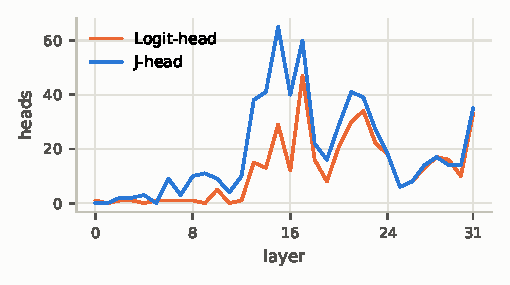
\includegraphics[width=0.55\textwidth]{figures/layers_simple.pdf}
\caption{Lexical task heads per layer under each readout, summed over the head sets of all simple tasks and styles, at the last prompt token.}
\label{fig:layers-simple}
\end{figure}

\begin{figure}[H]
\centering
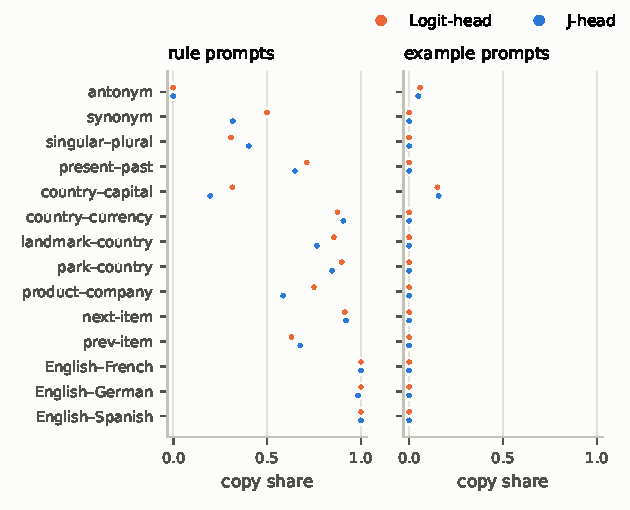
\includegraphics[width=0.7\textwidth]{figures/copy_share_simple.pdf}
\caption{Copy share of each simple-task head set (Sec.~\ref{sec:measures}): the share of prompts on which a head's matched terms occur in the prompt text, averaged over the set.}
\label{fig:copy-simple}
\end{figure}

\begin{figure}[H]
\centering
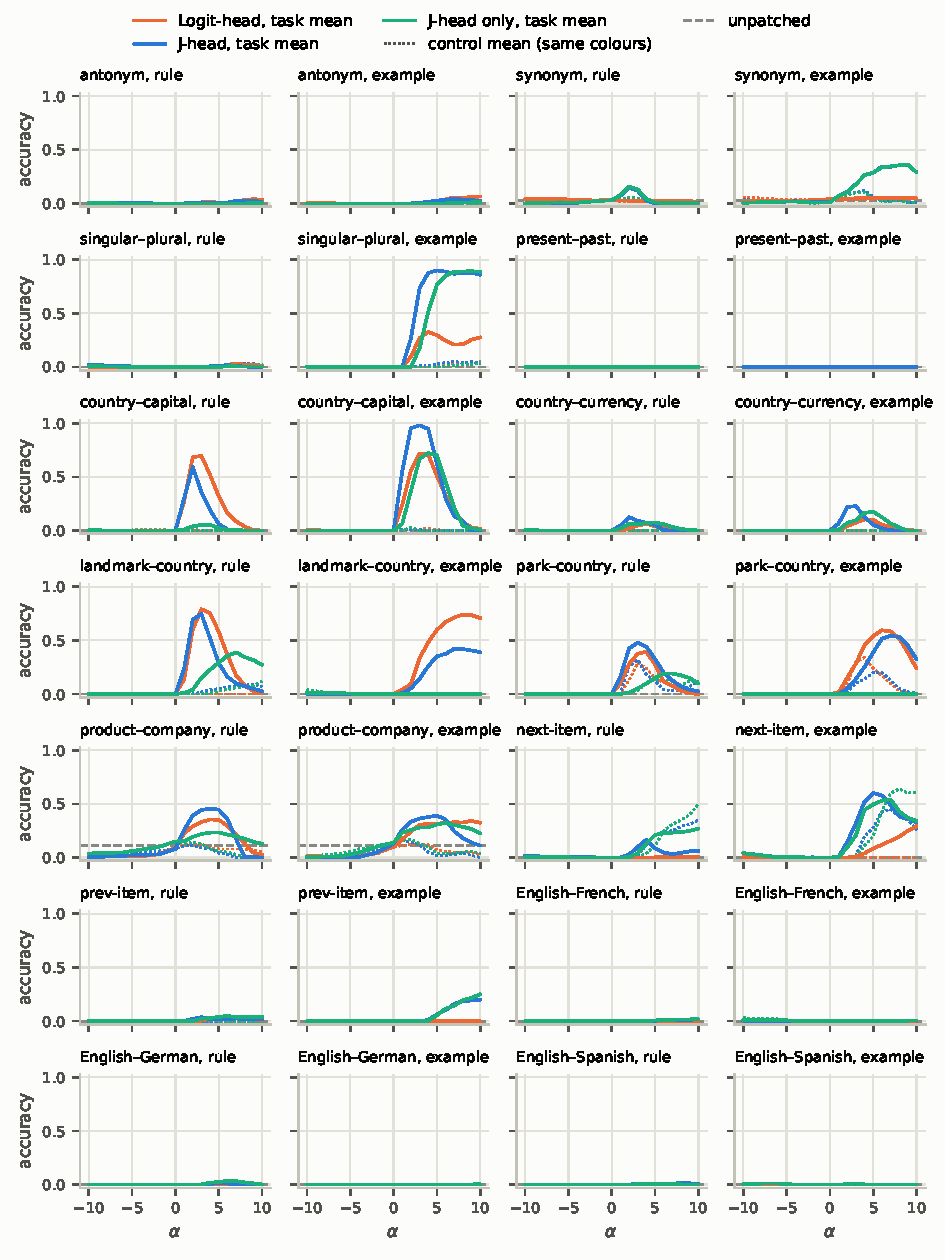
\includegraphics[width=\textwidth]{figures/patching_simple.pdf}
\caption{E1 causal check: accuracy on the 100 patched items of each task against $\alpha$, with each style's head set patched with means of the same style, averaged over the style's five source wordings. Solid: the head set's mean over the task's prompts; dotted: the control mean at the same heads; dashed: unpatched accuracy.}
\label{fig:patch-simple}
\end{figure}

\begin{figure}[H]
\centering
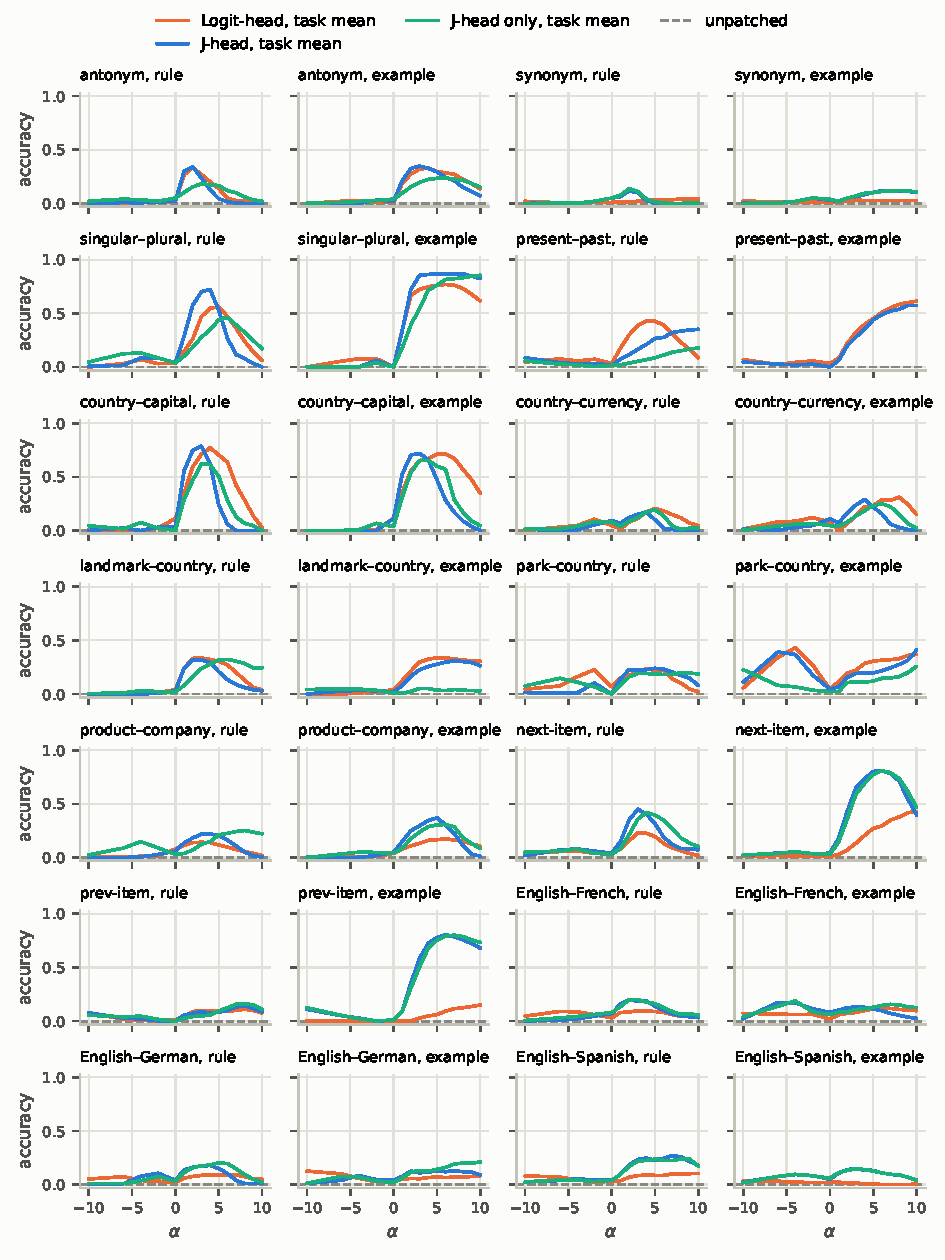
\includegraphics[width=\textwidth]{figures/patching_simple_wrong.pdf}
\caption{E1, second causal check, as Figure~\ref{fig:patch-simple}, with the wrongly answered 1-shot prompts patched. No control mean.}
\label{fig:patch-simple-wrong}
\end{figure}

% =====================================================================
\section{E1b: Heads from all five instruction templates}\label{sec:consensus}

\begin{hypothesis}[several wordings]\label{h:consensus}
On the simple tasks, rule-style lexical task heads that meet Definition~\ref{def:lth} under every instruction template, not only under the most accurate one, carry the task more strongly: patched as in E1, they raise accuracy more than the heads of the most accurate template, and the control mean does not raise it more. \emph{Falsified} if, under each readout and in each causal check, their causal effect is larger on at most half of the 14 tasks, or if their larger effects come with a larger effect of the control mean.
\end{hypothesis}

\subsection{Design}
\paragraph{Question.} H\ref{h:consensus}: do the rule-style lexical task heads that every instruction template yields carry the task more strongly than those of the most accurate template? A head that names the task under one template may be copying words of that template; one that names it under all five is less tied to a wording.

\paragraph{Conditions.} 14 tasks $\times$ the rule style $\times$ 2 readouts (Logit-head, J-head). The heads found only by J-head and the example style are not part of E1b.

\paragraph{Procedure.}
\begin{enumerate}
\item \emph{Identification prompts}: for each of the five instruction templates separately, its first 100 prompts in $P^{+}$ (all of them where fewer are answered correctly).
\item \emph{Head sets}: under each readout, a head is in the consensus set if it meets Definition~\ref{def:lth} on the prompts of all five templates. The rule-style set of E1 comes from one of the five templates, so the consensus set is contained in it.
\item \emph{Measures}: head count, and the heads the set shares with the E1 set.
\item \emph{Causal checks}: both checks of E1, unchanged (patched items, means of both styles, control mean, $\alpha$, scoring); only the head sets differ.
\item \emph{Comparison}: per task, readout and check, the causal effect of the consensus set against that of the E1 rule-style set with rule-style means, and in the first check the same for the control mean.
\end{enumerate}

\paragraph{Output.} Head sets (Table~\ref{tab:heads-consensus}); causal effects of the E1 set and of the consensus set side by side, in the first check (Table~\ref{tab:effects-consensus}), with the control mean (Table~\ref{tab:effects-consensus-control}), and in the second check (Table~\ref{tab:effects-consensus-wrong}). The tables also hold the sets of Sec.~\ref{sec:k13}.

\subsection{Results}\label{sec:res-consensus}
\paragraph{Head sets} (Table~\ref{tab:heads-consensus}). The consensus sets ($k=5$) keep three fifths of the Logit-head heads of E1 and just over half of the J-head heads. They keep least on next-item, singular--plural and park--country under both readouts and on synonym under J-head; synonym has no Logit-head consensus set, so it is not patched.

\paragraph{Causal checks} (Tables~\ref{tab:effects-consensus}, \ref{tab:effects-consensus-control} and~\ref{tab:effects-consensus-wrong}). The consensus sets give the largest effect of the four sets (E1's and those for $k=1$, 3 and 5) on tasks where the E1 sets were already effective. In the first check, these are country--capital and park--country under both readouts, product--company under Logit-head and landmark--country under J-head, with 7 to 26 more items than the E1 sets, and product--company under J-head, by less than one item; in the second, country--capital, park--country and product--company under both readouts, with 1 to 5 more items. Elsewhere the consensus sets are ahead of the E1 sets by less than three items: on prev-item under J-head in the first check, and in the second on English--French and English--Spanish under Logit-head and on country--currency and synonym under J-head. The control mean rises with them by more than three items only at the J-head set of park--country. On most other tasks the consensus sets have a smaller effect than the E1 sets, most in the second check on singular--plural and next-item and under J-head on the translation tasks. On next-item, the J-head set's gain in the first check disappears together with that of the control mean.

\paragraph{Hypothesis.} H\ref{h:consensus} is falsified: under each readout and in each check, the consensus sets raise accuracy more than the E1 sets on at most 5 of the 14 tasks, and by more than three items on at most 3.

\begin{table}[H]
\centering\footnotesize\setlength{\tabcolsep}{3pt}
% Generated by scripts/results_tex.py from results/.
\begin{tabular}{@{}lcccccccc@{}}
\toprule
 & \multicolumn{4}{c}{L} & \multicolumn{4}{c}{J} \\
\cmidrule(lr){2-5}\cmidrule(lr){6-9}
Task & E1 & $k=1$ & $k=3$ & $k=5$ & E1 & $k=1$ & $k=3$ & $k=5$ \\
\midrule
antonym & 14 (1.4) & 30 (2.9) & 17 (1.7) & 11 (1.1) & 21 (2.1) & 36 (3.5) & 22 (2.1) & 13 (1.3) \\
synonym & 2 (0.2) & 11 (1.1) & 2 (0.2) & 0 (0.0) & 22 (2.1) & 49 (4.8) & 21 (2.1) & 7 (0.7) \\
singular--plural & 20 (2.0) & 38 (3.7) & 17 (1.7) & 7 (0.7) & 24 (2.3) & 41 (4.0) & 23 (2.2) & 8 (0.8) \\
present--past & 10 (1.0) & 17 (1.7) & 10 (1.0) & 4 (0.4) & 7 (0.7) & 19 (1.9) & 7 (0.7) & 3 (0.3) \\
country--capital & 21 (2.1) & 36 (3.5) & 22 (2.1) & 14 (1.4) & 35 (3.4) & 62 (6.1) & 36 (3.5) & 25 (2.4) \\
country--currency & 17 (1.7) & 22 (2.1) & 16 (1.6) & 14 (1.4) & 33 (3.2) & 48 (4.7) & 31 (3.0) & 23 (2.2) \\
landmark--country & 23 (2.2) & 38 (3.7) & 25 (2.4) & 19 (1.9) & 27 (2.6) & 64 (6.2) & 29 (2.8) & 15 (1.5) \\
park--country & 24 (2.3) & 38 (3.7) & 24 (2.3) & 11 (1.1) & 24 (2.3) & 50 (4.9) & 25 (2.4) & 12 (1.2) \\
product--company & 30 (2.9) & 42 (4.1) & 28 (2.7) & 20 (2.0) & 40 (3.9) & 74 (7.2) & 37 (3.6) & 25 (2.4) \\
next-item & 35 (3.4) & 45 (4.4) & 20 (2.0) & 11 (1.1) & 47 (4.6) & 60 (5.9) & 28 (2.7) & 13 (1.3) \\
prev-item & 20 (2.0) & 36 (3.5) & 21 (2.1) & 11 (1.1) & 35 (3.4) & 71 (6.9) & 33 (3.2) & 20 (2.0) \\
English--French & 11 (1.1) & 15 (1.5) & 10 (1.0) & 10 (1.0) & 22 (2.1) & 40 (3.9) & 18 (1.8) & 13 (1.3) \\
English--German & 7 (0.7) & 13 (1.3) & 9 (0.9) & 7 (0.7) & 19 (1.9) & 34 (3.3) & 17 (1.7) & 14 (1.4) \\
English--Spanish & 6 (0.6) & 8 (0.8) & 6 (0.6) & 5 (0.5) & 14 (1.4) & 24 (2.3) & 16 (1.6) & 8 (0.8) \\
\midrule
Mean per task & 17.1 (1.7) & 27.8 (2.7) & 16.2 (1.6) & 10.3 (1.0) & 26.4 (2.6) & 48.0 (4.7) & 24.5 (2.4) & 14.2 (1.4) \\
Distinct, all tasks & 124 (12.1) & 182 (17.8) & 112 (10.9) & 84 (8.2) & 179 (17.5) & 270 (26.4) & 157 (15.3) & 105 (10.3) \\
\bottomrule
\end{tabular}

\caption{E1b: rule-style head sets under Logit-head (L) and J-head (J): from the most accurate instruction template (E1, Table~\ref{tab:heads-simple}), and the heads that meet Definition~\ref{def:lth} under at least $k$ of the five templates. Each cell: number of heads and, in brackets, its share of the model's 1,024 heads in \%. Distinct: heads in the set of at least one task. The set for $k=1$ contains the E1 set and the set for $k=5$ is contained in it; of the heads in the sets for $k=3$, summed over tasks, 198 of 227 (L) and 300 of 343 (J) are in the E1 sets.}
\label{tab:heads-consensus}
\end{table}

\begin{table}[H]
\centering\footnotesize
% Generated by scripts/results_tex.py from results/.
\begin{tabular}{@{}lcccccccccccc@{}}
\toprule
 & \multicolumn{6}{c}{First check} & \multicolumn{6}{c}{Second check} \\
\cmidrule(lr){2-7}\cmidrule(lr){8-13}
 & \multicolumn{2}{c}{L} & \multicolumn{2}{c}{J} & \multicolumn{2}{c}{J only} & \multicolumn{2}{c}{L} & \multicolumn{2}{c}{J} & \multicolumn{2}{c}{J only} \\
\cmidrule(lr){2-3}\cmidrule(lr){4-5}\cmidrule(lr){6-7}\cmidrule(lr){8-9}\cmidrule(lr){10-11}\cmidrule(lr){12-13}
Task & E1 & E1b & E1 & E1b & E1 & E1b & E1 & E1b & E1 & E1b & E1 & E1b \\
\midrule
antonym & 0.04 & 0.02 & 0.03 & 0.01 & 0.01 & 0.00 & 0.33 & 0.29 & 0.34 & 0.28 & 0.18 & 0.08 \\
synonym & 0.01 & -- & 0.12 & 0.07 & 0.13 & 0.07 & 0.04 & -- & 0.12 & 0.12 & 0.14 & 0.12 \\
singular--plural & 0.03 & 0.00 & 0.02 & 0.01 & 0.01 & 0.00 & 0.56 & 0.35 & 0.72 & 0.42 & 0.46 & 0.23 \\
present--past & 0.00 & 0.00 & 0.00 & 0.00 & 0.00 & -- & 0.43 & 0.40 & 0.35 & 0.29 & 0.18 & -- \\
country--capital & 0.70 & 0.80 & 0.59 & 0.75 & 0.05 & 0.34 & 0.77 & 0.82 & 0.79 & 0.84 & 0.62 & 0.68 \\
country--currency & 0.06 & 0.06 & 0.12 & 0.12 & 0.07 & 0.07 & 0.21 & 0.18 & 0.17 & 0.18 & 0.19 & 0.18 \\
landmark--country & 0.79 & 0.71 & 0.75 & 0.93 & 0.39 & 0.27 & 0.34 & 0.33 & 0.32 & 0.31 & 0.32 & 0.28 \\
park--country & 0.39 & 0.65 & 0.48 & 0.71 & 0.19 & 0.08 & 0.24 & 0.33 & 0.24 & 0.29 & 0.20 & 0.24 \\
product--company & 0.24 & 0.31 & 0.35 & 0.35 & 0.12 & 0.12 & 0.14 & 0.16 & 0.22 & 0.27 & 0.25 & 0.33 \\
next-item & 0.01 & 0.00 & 0.17 & 0.01 & 0.27 & 0.02 & 0.23 & 0.10 & 0.45 & 0.17 & 0.42 & 0.15 \\
prev-item & 0.04 & 0.00 & 0.04 & 0.06 & 0.05 & 0.13 & 0.11 & 0.05 & 0.14 & 0.09 & 0.16 & 0.14 \\
English--French & 0.00 & 0.00 & 0.02 & 0.00 & 0.02 & 0.00 & 0.10 & 0.10 & 0.20 & 0.13 & 0.20 & 0.13 \\
English--German & 0.00 & 0.00 & 0.01 & 0.00 & 0.04 & 0.00 & 0.09 & 0.09 & 0.18 & 0.13 & 0.20 & 0.18 \\
English--Spanish & 0.00 & 0.00 & 0.01 & 0.01 & 0.01 & 0.01 & 0.10 & 0.11 & 0.27 & 0.19 & 0.24 & 0.18 \\
\bottomrule
\end{tabular}

\caption{E1b, first causal check: causal effect of the rule-style head sets of Table~\ref{tab:heads-consensus} with rule-style means, as in Table~\ref{tab:effects-simple}; 100 patched items per task. --: empty set.}
\label{tab:effects-consensus}
\end{table}

\begin{table}[H]
\centering\footnotesize
% Generated by scripts/results_tex.py from results/.
\begin{tabular}{@{}lcccccccc@{}}
\toprule
 & \multicolumn{4}{c}{L} & \multicolumn{4}{c}{J} \\
\cmidrule(lr){2-5}\cmidrule(lr){6-9}
Task & E1 & $k=1$ & $k=3$ & $k=5$ & E1 & $k=1$ & $k=3$ & $k=5$ \\
\midrule
antonym & 0.00 & 0.04 & 0.04 & 0.00 & 0.00 & 0.00 & 0.01 & 0.00 \\
synonym & 0.01 & 0.01 & 0.01 & -- & 0.02 & 0.02 & 0.02 & 0.05 \\
singular--plural & 0.00 & 0.02 & 0.00 & 0.00 & 0.03 & 0.02 & 0.02 & 0.00 \\
present--past & 0.00 & 0.00 & 0.00 & 0.00 & 0.00 & 0.00 & 0.00 & 0.00 \\
country--capital & 0.01 & 0.01 & 0.01 & 0.01 & 0.00 & 0.00 & 0.01 & 0.01 \\
country--currency & 0.00 & 0.00 & 0.00 & 0.00 & 0.00 & 0.00 & 0.00 & 0.00 \\
landmark--country & 0.00 & 0.00 & 0.00 & 0.00 & 0.09 & 0.00 & 0.14 & 0.02 \\
park--country & 0.29 & 0.24 & 0.28 & 0.21 & 0.32 & 0.21 & 0.29 & 0.43 \\
product--company & 0.01 & 0.01 & 0.01 & 0.02 & 0.00 & $-$0.02 & 0.01 & 0.01 \\
next-item & 0.00 & 0.00 & 0.01 & 0.00 & 0.35 & 0.27 & 0.34 & 0.03 \\
prev-item & 0.00 & 0.00 & 0.00 & 0.00 & 0.00 & 0.02 & 0.01 & 0.00 \\
English--French & 0.01 & 0.03 & 0.01 & 0.01 & 0.00 & 0.06 & 0.01 & 0.02 \\
English--German & 0.00 & 0.00 & 0.00 & 0.00 & 0.00 & 0.00 & 0.00 & 0.00 \\
English--Spanish & 0.00 & 0.00 & 0.00 & 0.00 & 0.00 & 0.00 & 0.00 & 0.00 \\
\bottomrule
\end{tabular}

\caption{E1b, first causal check: causal effect of the control mean at the head sets of Table~\ref{tab:heads-consensus}, as the control columns of Table~\ref{tab:effects-simple}.}
\label{tab:effects-consensus-control}
\end{table}

\begin{table}[H]
\centering\footnotesize
% Generated by scripts/results_tex.py from results/.
\begin{tabular}{@{}lrcccccccc@{}}
\toprule
 & & \multicolumn{4}{c}{L} & \multicolumn{4}{c}{J} \\
\cmidrule(lr){3-6}\cmidrule(lr){7-10}
Task & Items & E1 & $k=1$ & $k=3$ & $k=5$ & E1 & $k=1$ & $k=3$ & $k=5$ \\
\midrule
antonym & 100 & 0.33 & 0.28 & 0.31 & 0.29 & 0.34 & 0.36 & 0.35 & 0.28 \\
synonym & 100 & 0.04 & 0.08 & 0.04 & -- & 0.12 & 0.10 & 0.13 & 0.12 \\
singular--plural & 26 & 0.56 & 0.58 & 0.69 & 0.35 & 0.72 & 0.67 & 0.75 & 0.42 \\
present--past & 61 & 0.43 & 0.51 & 0.40 & 0.40 & 0.35 & 0.64 & 0.35 & 0.29 \\
country--capital & 27 & 0.77 & 0.77 & 0.81 & 0.82 & 0.79 & 0.81 & 0.79 & 0.84 \\
country--currency & 65 & 0.21 & 0.22 & 0.19 & 0.18 & 0.17 & 0.17 & 0.18 & 0.18 \\
landmark--country & 100 & 0.34 & 0.31 & 0.32 & 0.33 & 0.32 & 0.31 & 0.29 & 0.31 \\
park--country & 45 & 0.24 & 0.24 & 0.24 & 0.33 & 0.24 & 0.24 & 0.23 & 0.29 \\
product--company & 100 & 0.14 & 0.14 & 0.15 & 0.16 & 0.22 & 0.26 & 0.21 & 0.27 \\
next-item & 100 & 0.23 & 0.32 & 0.09 & 0.10 & 0.45 & 0.50 & 0.49 & 0.17 \\
prev-item & 100 & 0.11 & 0.12 & 0.15 & 0.05 & 0.14 & 0.12 & 0.15 & 0.09 \\
English--French & 100 & 0.10 & 0.11 & 0.10 & 0.10 & 0.20 & 0.25 & 0.15 & 0.13 \\
English--German & 100 & 0.09 & 0.10 & 0.09 & 0.09 & 0.18 & 0.20 & 0.15 & 0.13 \\
English--Spanish & 100 & 0.10 & 0.13 & 0.10 & 0.11 & 0.27 & 0.27 & 0.25 & 0.19 \\
\bottomrule
\end{tabular}

\caption{E1b, second causal check: causal effect of the head sets of Table~\ref{tab:heads-consensus} with rule-style means, as in Table~\ref{tab:effects-simple-wrong}. Items: the wrongly answered 1-shot prompts patched; the baseline is 0.}
\label{tab:effects-consensus-wrong}
\end{table}


\begin{figure}[H]
\centering
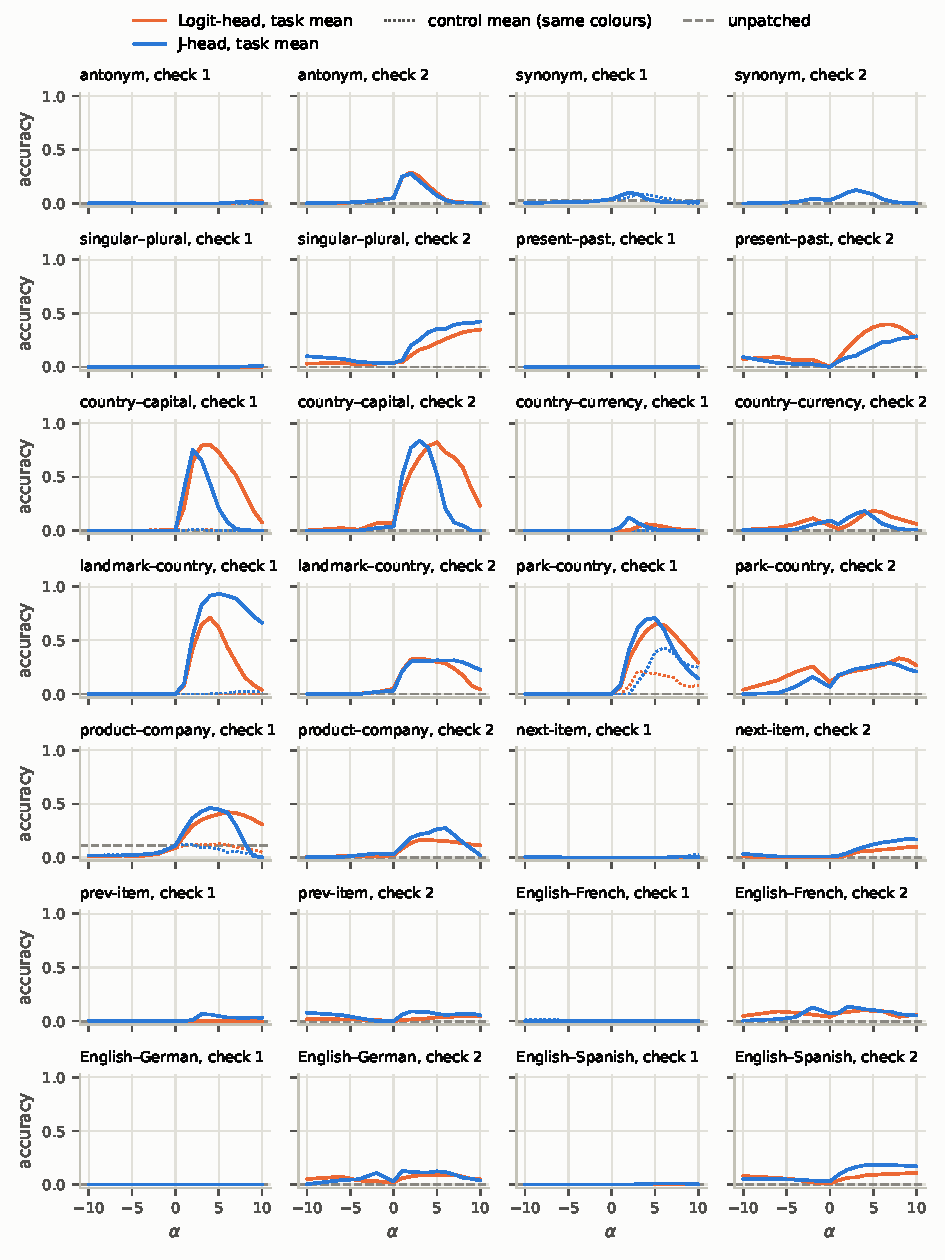
\includegraphics[width=\textwidth]{figures/patching_consensus_k5.pdf}
\caption{E1b, consensus sets ($k=5$): accuracy against $\alpha$ for the rule-style sets with rule-style means, averaged over the five instruction templates. For each task, the first check (zero-shot prompts of the first 100 items answered correctly with one shot) and the second (1-shot prompts answered wrongly; no control mean). Solid: the head set's mean over the task's prompts; dotted: the control mean at the same heads; dashed: unpatched accuracy. Synonym has no Logit-head consensus set.}
\label{fig:patch-consensus}
\end{figure}

% =====================================================================
\section{E1b, exploratory: heads from at least one or three templates}\label{sec:k13}
\subsection{Design}
\paragraph{Question.} After the result of H\ref{h:consensus}, we ask how the causal effect changes when fewer templates are required. This question has no hypothesis, and we report it as exploratory.

\paragraph{Design.} As in Sec.~\ref{sec:consensus}, with a head in the set for $k$ if it meets Definition~\ref{def:lth} on the prompts of at least $k$ of the five templates, for $k\in\{1,3\}$. The set for $k=1$ (the union of the five templates' sets) contains the E1 set; the set for $k=3$ neither contains it nor is contained in it. Head sets and causal effects are in Tables~\ref{tab:heads-consensus}--\ref{tab:effects-consensus-wrong}, beside those of the consensus sets.

\subsection{Results}\label{sec:res-k13}
\paragraph{Head sets} (Table~\ref{tab:heads-consensus}). The three requirements give sets of very different sizes, all small against the model's 1,024 heads: even the union averages under 5\% of them per task under J-head, and its sets of all tasks together cover about a quarter. Per task on average, the union ($k=1$) has about 1.6 times as many heads as the E1 set under Logit-head and 1.8 times under J-head; counted as distinct heads over all tasks, about 1.5 times under both. The sets for $k=3$ are about as large as the E1 sets, and seven in eight of their heads are E1 heads.

\paragraph{Causal checks} (Tables~\ref{tab:effects-consensus}, \ref{tab:effects-consensus-control} and~\ref{tab:effects-consensus-wrong}). No requirement gives the largest effect on most tasks; which one does depends on the task.

The union raises J-head's effect on three tasks where the E1 set had little: synonym and prev-item in the first check, and present--past in both, where the first check goes from no effect to 16 items and the second roughly doubles. In the first check, the control mean at these sets stays within two items of zero. The patched present--past prompts are answered with the past tense of the given verb; at the mean and $\alpha$ with the highest accuracy, 94 of the 100 replies differ, so the gain is not one answer repeated. In the first check it is largest at the largest $\alpha$, 10. Two further gains of the union are not specific to the task: on English--French the control mean rises almost as much, and on next-item the gain stays below that of the control mean. Under Logit-head the union lowers the first check's effect on park--country, landmark--country and product--company, and raises the second check's on next-item and present--past.

The sets for $k=3$ behave like the E1 sets they mostly consist of. They gain on some tasks and lose on as many, and the union's effect on present--past is gone. Their largest change is on next-item under Logit-head, whose second-check effect falls by more than half; at the J-head set of landmark--country, the control mean rises.

The three requirements thus trade off against each other. Heads that every template yields carry country--capital, park--country and product--company more strongly. Heads that only one or two templates yield add to J-head's effect on present--past, prev-item and synonym, and requiring three templates already removes them. The number of templates under which a head is found is therefore not by itself a measure of how strongly it carries the task.


\begin{figure}[H]
\centering
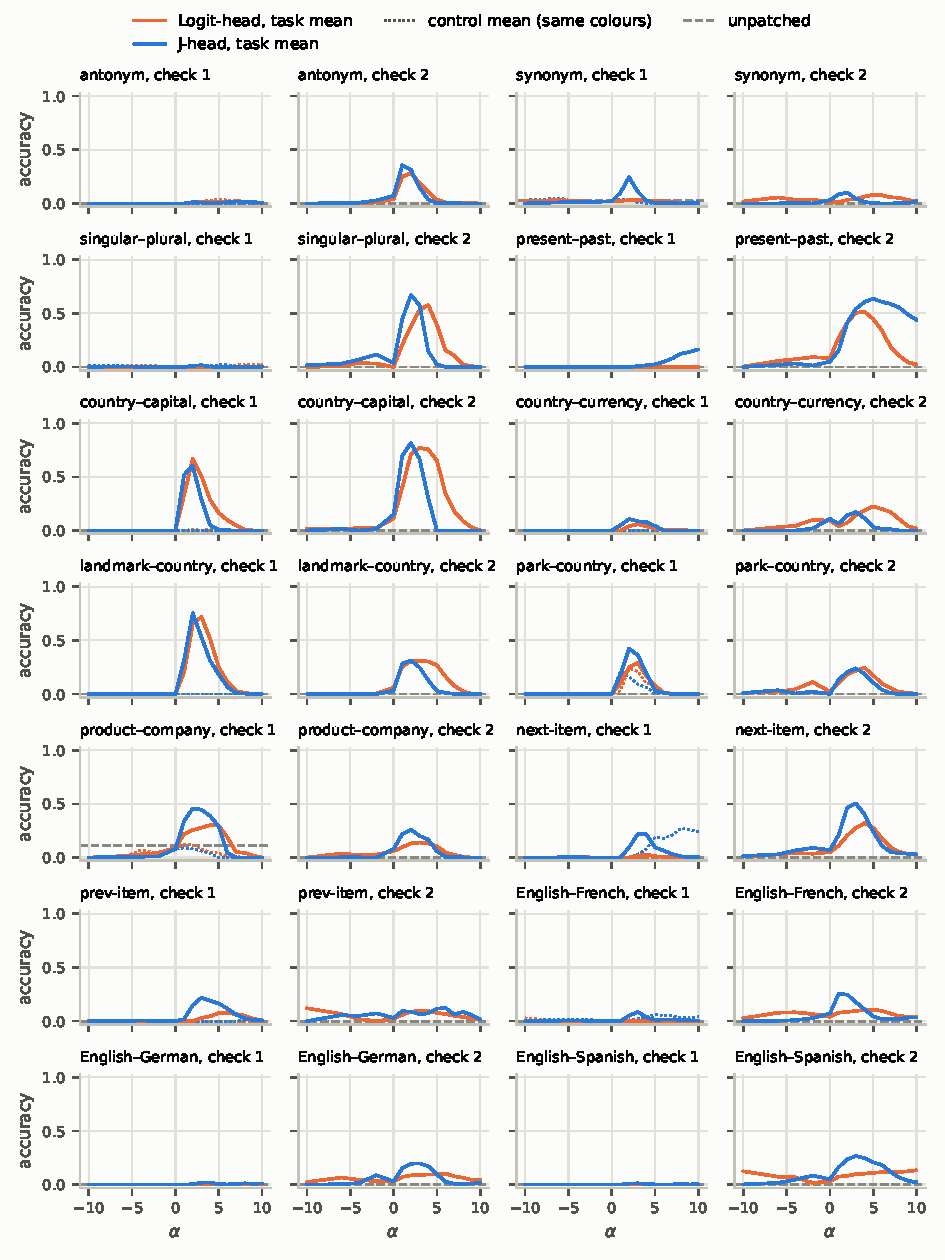
\includegraphics[width=\textwidth]{figures/patching_consensus_k1.pdf}
\caption{E1b, heads from at least one template ($k=1$, the union), as Figure~\ref{fig:patch-consensus}.}
\label{fig:patch-k1}
\end{figure}

\begin{figure}[H]
\centering
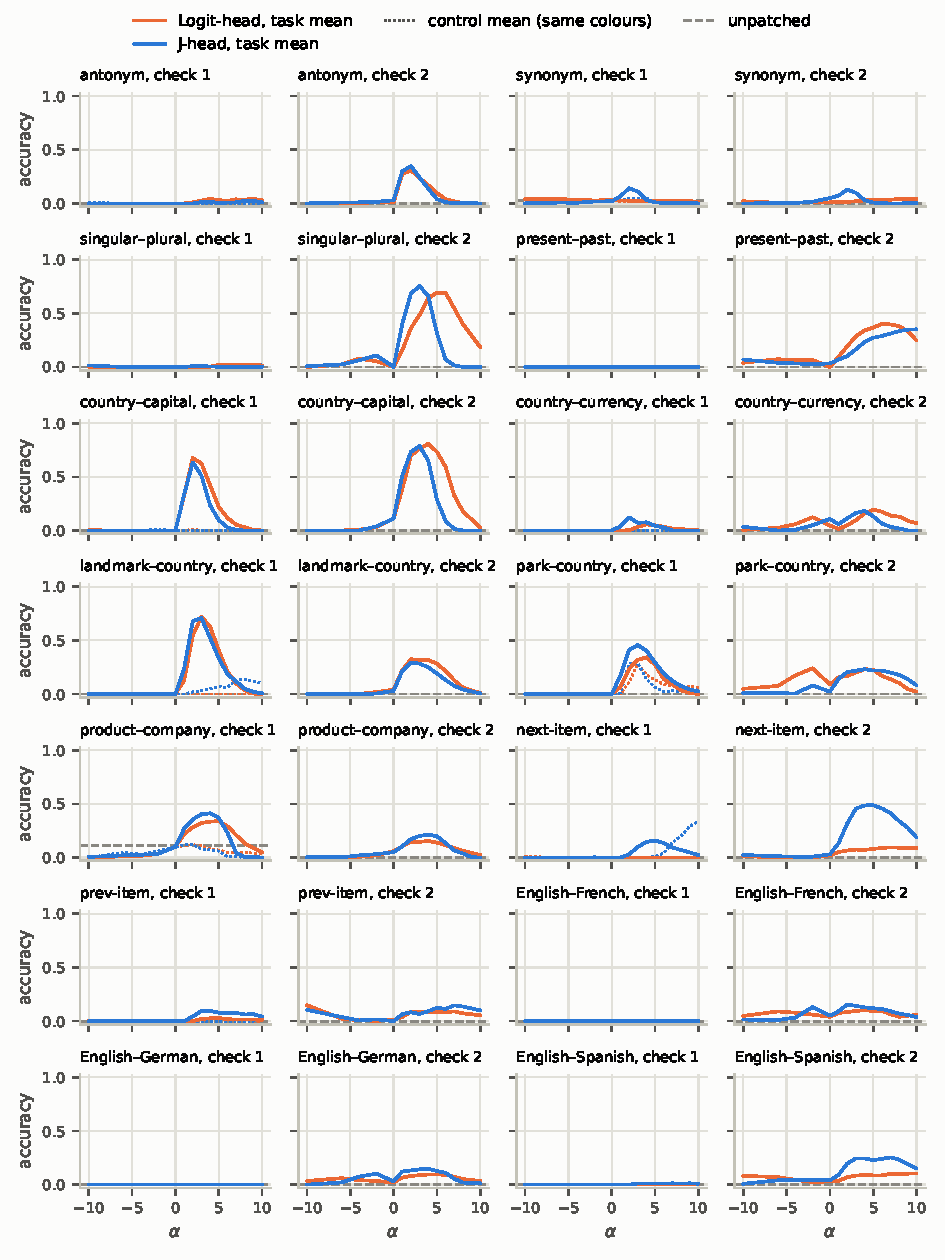
\includegraphics[width=\textwidth]{figures/patching_consensus_k3.pdf}
\caption{E1b, heads from at least three templates ($k=3$), as Figure~\ref{fig:patch-consensus}.}
\label{fig:patch-k3}
\end{figure}

% =====================================================================
\section{Shared heads of the union}\label{sec:shared}
\ph{S1}{Shared heads of the union}{J-head $k=1$ sets restricted to heads in the union sets of at least two tasks; both checks, all tasks (da04856).}

\begin{figure}[H]
\centering
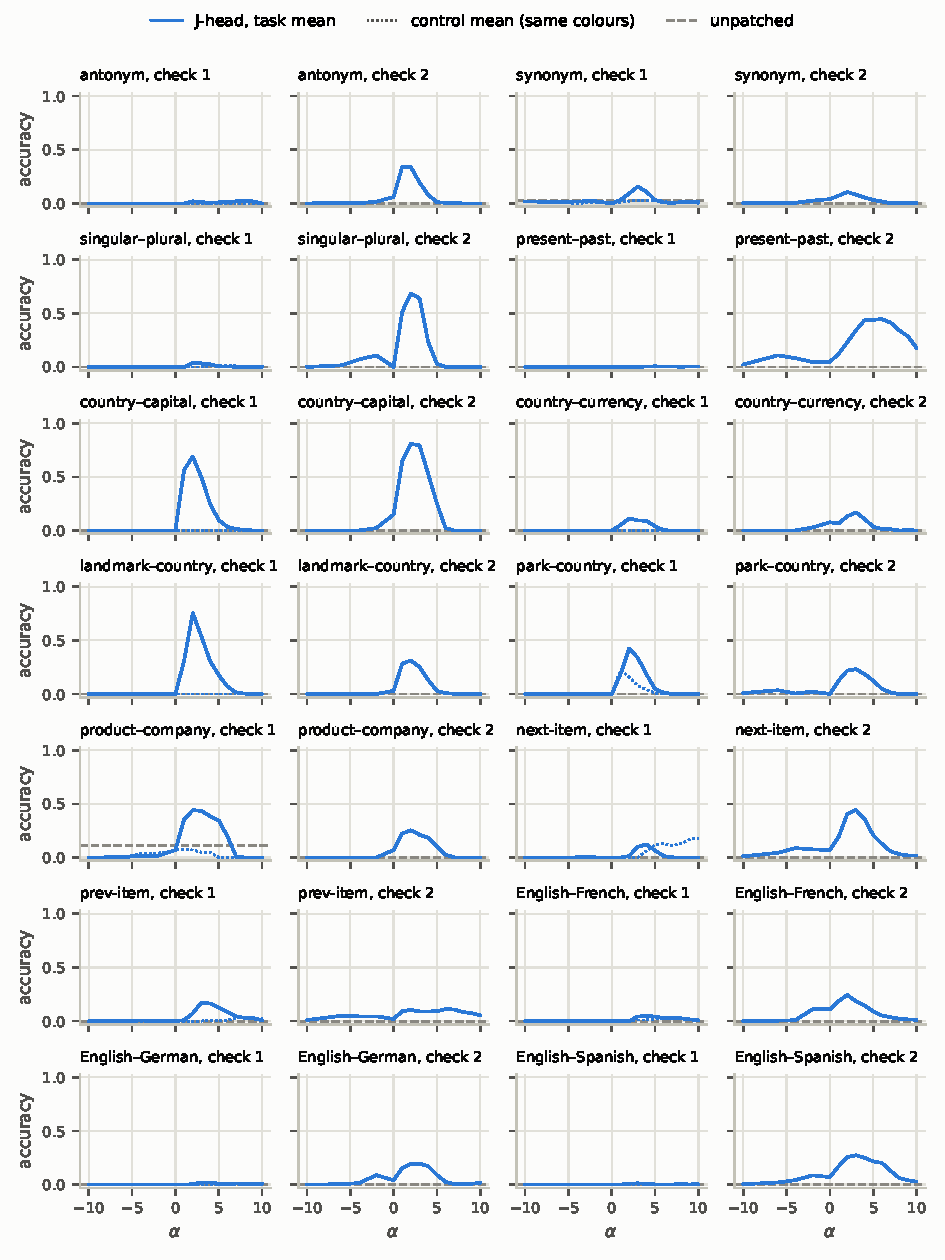
\includegraphics[width=\textwidth]{figures/patching_shared.pdf}
\caption{J-head union sets ($k=1$) restricted to the heads that are also in the union set of at least one other task, as Figure~\ref{fig:patch-consensus}.}
\label{fig:patch-shared}
\end{figure}

% =====================================================================
\section{Present--past: the union's four unshared heads}\label{sec:pp4}
\ph{S2}{Present--past: the union's four unshared heads}{The 4 heads only present--past's J-head union set contains (L19H10, L19H24, L20H28, L21H9); both checks, present--past only (c8c6fb8).}

\begin{figure}[H]
\centering
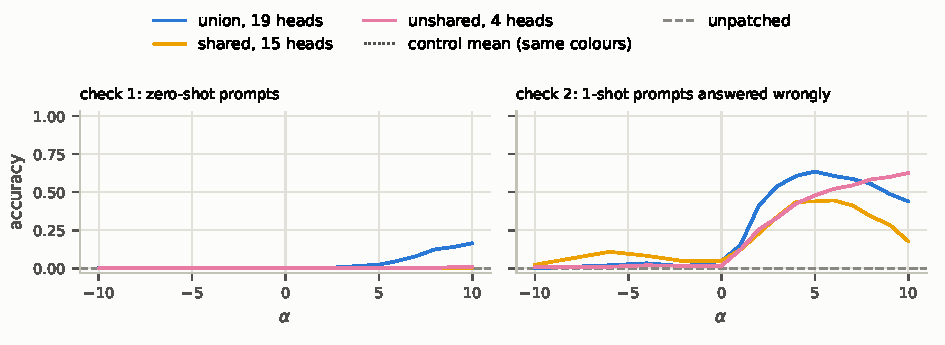
\includegraphics[width=\textwidth]{figures/patching_pp_unshared.pdf}
\caption{Present--past, J-head, rule-style means averaged over the five instruction templates: the union set ($k=1$, 19 heads), its 15 heads that are also in another task's union set (shared), and its 4 other heads (unshared: L19H10, L19H24, L20H28, L21H9). Left: first check (100 items); right: second check (61 items, no control mean). Solid: task mean; dotted: control mean at the same heads; dashed: unpatched accuracy.}
\label{fig:patch-pp-unshared}
\end{figure}

% =====================================================================
\section{Patched replies by kind}\label{sec:replies}
\ph{S3}{Patched replies by kind}{Each patched reply sorted by kind, present--past and all tasks; \texttt{notebooks/patching\_outputs.py} (0239820, 1cfc886).}

% =====================================================================
\section{Retrieval heads}\label{sec:retrieval}
\ph{S4}{Retrieval heads}{Yang et al.'s retrieval heads (Definition~\ref{def:lth} with the answer token as target) and their overlap with every lexical set, against layer-matched chance (1f189a7).}

% =====================================================================
\section{Present--past: L21H9 and the other three heads}\label{sec:pp-split}
\ph{S5}{Present--past: L21H9 and the other three heads}{L21H9 alone, and L19H10, L19H24, L20H28 alone; both checks (42a8033).}

\begin{figure}[H]
\centering
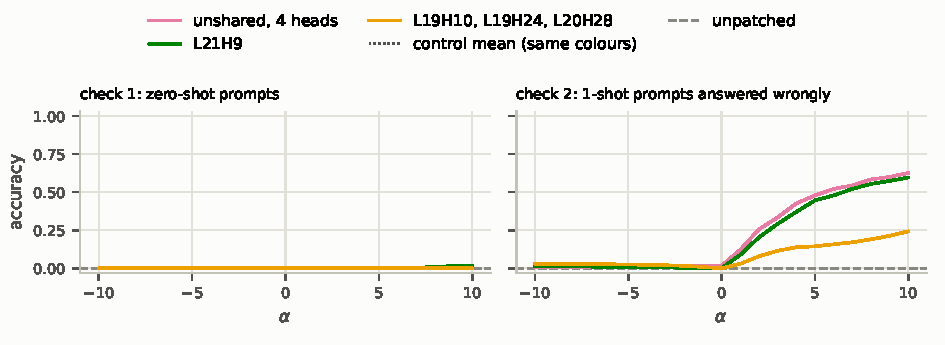
\includegraphics[width=\textwidth]{figures/patching_pp_split.pdf}
\caption{Present--past, as Figure~\ref{fig:patch-pp-unshared}: the 4 unshared heads, L21H9 alone, and the other three (L19H10, L19H24, L20H28) alone.}
\label{fig:patch-pp-split}
\end{figure}

% =====================================================================
\section{The union without retrieval heads}\label{sec:noretrieval}
\ph{S6}{The union without retrieval heads}{$k=1$ sets minus every retrieval head of the task; both checks, all tasks (2b0e939).}

\begin{figure}[H]
\centering
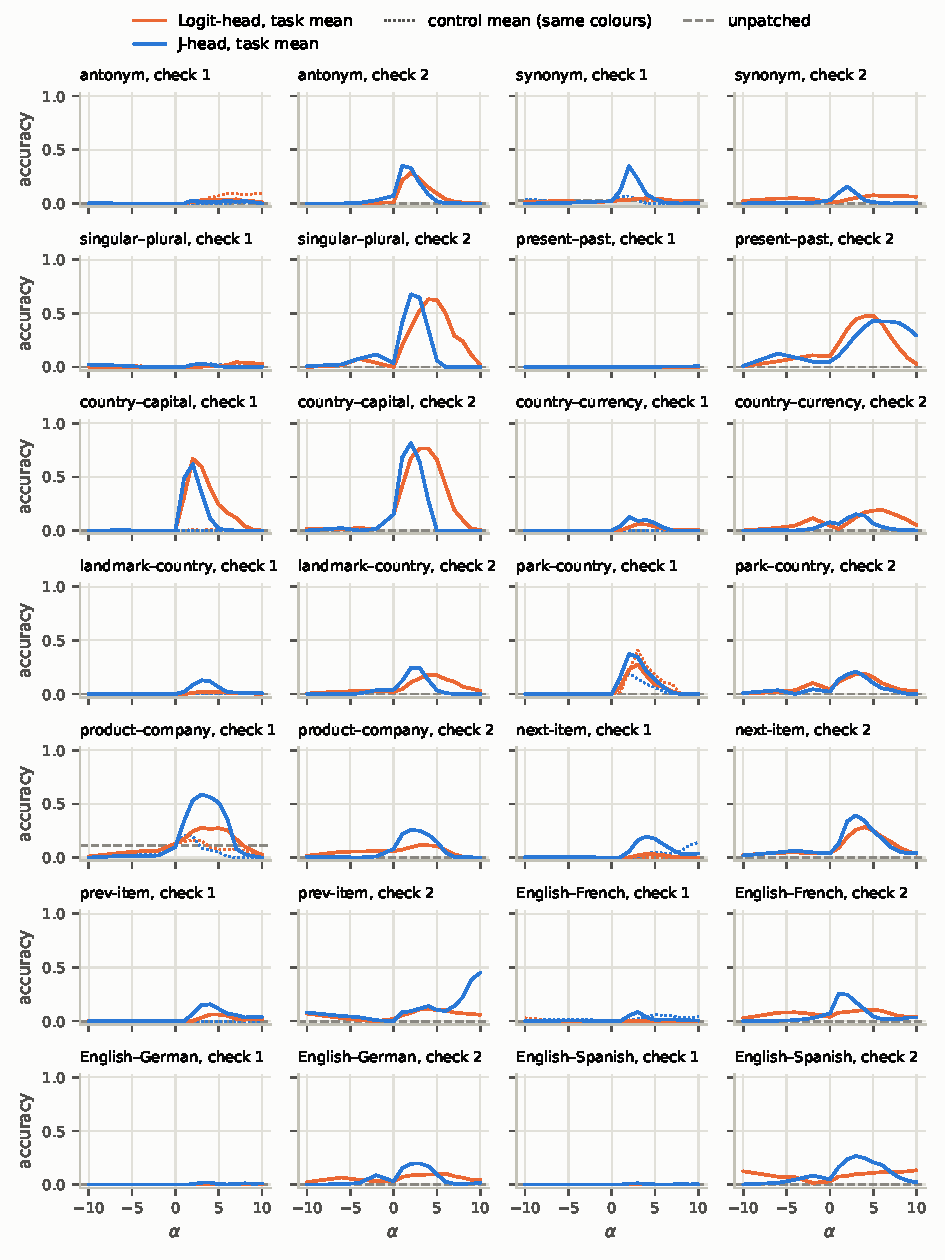
\includegraphics[width=\textwidth]{figures/patching_noretrieval.pdf}
\caption{Union sets ($k=1$) without the task's retrieval heads (found under any template and either readout), as Figure~\ref{fig:patch-consensus}.}
\label{fig:patch-noretrieval}
\end{figure}

% =====================================================================
\section{Head sets of equal size}\label{sec:sized}
\subsection{Design}
\paragraph{Question.} The head sets compared so far differ in size: the J-head sets are larger than the Logit-head sets on 23 of the 28 pairs of task and style (Sec.~\ref{sec:res-e1}), and the union of the five templates' sets has, per task on average, 1.6 to 1.8 times as many heads as the E1 set (Sec.~\ref{sec:res-k13}). A larger set changes more of the forward pass, so part of a difference in causal effect may come from the number of heads rather than from which heads are chosen. Do the differences between readouts and between template rules remain when every set has the same number of heads? The question was asked after the results of the earlier sections; it has no hypothesis, and we report it as exploratory.

\paragraph{Conditions.} 14 tasks $\times$ 2 readouts $\times$ 3 sizes, $N\in\{5,10,20\}$, $\times$ 4 selection rules: the rule of E1 (the most accurate instruction template for the rule style, 5 shots for the example style; both styles), and for the rule style the rules of E1b (at least $k$ of the five templates, $k\in\{1,3,5\}$).

\paragraph{Procedure.}
\begin{enumerate}
\item \emph{Ranking}: under each rule and readout, every head of the model is ranked by the quantity that Definition~\ref{def:lth} thresholds: its match rate on E1's identification prompts (E1), or the $k$-th highest of its match rates under the five templates (E1b). Ties are broken by the mean number of term tokens among the head's ten top tokens on the same prompts, then by layer and head. Recomputed from these rates, the threshold sets are those of E1 and E1b.
\item \emph{Head sets}: the first $N$ heads. Only heads that match on at least one prompt are ranked; where fewer than $N$ do, the set of size $N$ is not formed. This leaves out 37 of the 420 sets, all of size 10 or 20 except the J-head consensus set of present--past for $N=5$, most of them Logit-head sets of the translation tasks or consensus sets.
\item \emph{Measures}: how many of the $N$ heads meet the rule's threshold, and how many the Logit-head and J-head sets of the same rule and size share.
\item \emph{Causal checks}: both checks of E1 (patched items, control mean, scoring), each set patched with the means of its own style only, at nine of the fifteen values of $\alpha$: $-10$, $-4$, 2, 3, 4, 5, 6, 8 and 10. On the threshold sets of E1 and E1b, the highest accuracy over these nine values is within 0.05 of that over all fifteen, and within 0.02 on all but 4 of the 417 combinations of set, check and mean; for the comparison, the effects of the threshold sets are taken over the same nine values. A set equal to another of the same style and task is patched once.
\item \emph{Comparison}: the causal effect at equal size, in each check: J-head against Logit-head for each task, style, rule and $N$; each E1b rule against E1 for each task, readout and $N$. A difference seen between the threshold sets holds at equal size on a task if the same rule or readout has the larger effect at every $N$ for which both sets are formed.
\end{enumerate}

\paragraph{Output.} Head sets and measures (\texttt{results/sized}); causal effects at each size; accuracy against $\alpha$.

\subsection{Results}\label{sec:res-sized}
\paragraph{Head sets.} Where a threshold set has at least $N$ heads, the set of size $N$ is its $N$ highest-ranked heads; where it has fewer, the set adds the highest-ranked heads below the threshold. Below-threshold heads are therefore rare at size 5 and more frequent at size 20, more so under Logit-head, whose threshold sets are smaller. At each size, the Logit-head and J-head sets of the same rule share about three in five of their heads.

\paragraph{Readouts} (Table~\ref{tab:sized-summary}, Figures~\ref{fig:sized-readouts}--\ref{fig:sized-curves-n20-wrong}; effects in Tables~\ref{tab:sized-readouts}--\ref{tab:sized-readouts-control}, App.~\ref{app:sized}). J-head's advantage over Logit-head does not come from its larger sets. Taking the differences between the threshold sets of at least 0.05 (a descriptive cut, not part of the pre-stated comparison), J-head had the larger effect on most of them, in both styles and both checks, and on about two thirds of these it is larger at every size as well; on none is Logit-head. The few tasks on which Logit-head's threshold set had the larger effect do not keep it: on country--capital (rule style, first check) and present--past (rule style, second check) J-head is larger at every size. On country--capital, J-head's threshold set has more than one and a half times as many heads as Logit-head's, and its effect falls with the number of heads; on landmark--country and park--country (example style, first check) the order changes with the size.

\paragraph{Template rules} (Table~\ref{tab:sized-summary}, Figures~\ref{fig:sized-rules-logithead}--\ref{fig:sized-rule-curves-jhead-n20}; effects in Tables~\ref{tab:sized-rules} and~\ref{tab:sized-rules-wrong}, App.~\ref{app:sized}). Most differences between E1 and the rules of E1b change direction with the size, so they come from how many heads a rule selects, or from single heads, rather than from the rule. The few that hold at equal size are mostly about the consensus heads. In the second check, the consensus heads ($k=5$) have smaller effects than the E1 heads of the same number on several tasks, under J-head (antonym, singular--plural, next-item, English--German) and on singular--plural under Logit-head; few consensus sets of size 20 are formed, so this rests mostly on sizes 5 and 10. In the first check, the consensus heads have the larger effect on park--country under both readouts, a task on which the control mean also has large effects (below). The union's gain on present--past under J-head (Sec.~\ref{sec:res-k13}) holds as well, but at equal size it appears only at size 20 (below).

\paragraph{Size.} The effect does not grow steadily with the number of heads. On country--capital in the rule style, the five highest-ranked heads give the largest effect under both readouts; on next-item and prev-item in the second check, and on singular--plural in the example style, the sets of size 20 give the largest. Some single sizes stand out against both neighbours, such as the Logit-head example set of antonym at size 20 in the first check, which is the only antonym set with a large effect.

\paragraph{One head on present--past.} Under J-head with example-style heads, the first check has no effect at the threshold set, which has four heads, and a large one at sizes 5 and 10, with no effect of the control mean. The fifth head added, L15H1, matches on 7\% of the identification prompts, below the threshold; under Logit-head it matches on no present--past prompt of any wording. Read with J-head on the 1- and 5-shot prompts, its top tokens are mostly past participles (\emph{newly}, \emph{corrected}, \emph{recorded}, \emph{discovered}): the form of the answer rather than a name of the task, of which only ``previously'' is among them. Under instruction template 3 they name the past instead (\emph{past}, \emph{prior}, \emph{history}; match rate 0.53), under template 1 naming (\emph{name}, \emph{word}, \emph{called}). Patched alone with the example-style means (\texttt{results/pp\_L15H1}), L15H1 gives 0.80 in the first check and 0.76 in the second, close to the set of size 5 (0.87 and 0.80), against 0.00 and 0.57 for the four heads without it; the control mean has no effect. With the rule-style means it has none in either check (at most 0.06). The patched replies give the past tense of the verb on most items, the misses mostly its base form; the effect is still rising at $\alpha=10$, the end of the range. L15H1 is also in the J-head union set of size 20 for the rule style, the only rule-style set with an effect on present--past in the first check, but that set also holds the four unshared heads (Sec.~\ref{sec:pp4}).

\paragraph{Control mean} (dotted curves in Figures~\ref{fig:sized-curves-n5}, \ref{fig:sized-curves-n10} and~\ref{fig:sized-curves-n20}). On park--country the control mean has large effects at most sizes, in some sets as large as those of the task mean. The patched model answers with a title that begins with the country's name, such as ``Albania's Hidden Gem'', which the flexible score accepts. The control mean also comes close to or exceeds the task mean at the J-head example sets of singular--plural (size 5) and next-item (size 20). Effects on these tasks are not specific to the task.

Thus, at equal size, the difference between the readouts largely remains, while the differences between template rules mostly do not.

\begin{table}[H]
\centering\footnotesize
% Generated by scripts/sized_tex.py from results/.
\begin{tabular}{@{}lcccc@{}}
\toprule
 & \multicolumn{2}{c}{First check} & \multicolumn{2}{c}{Second check} \\
\cmidrule(lr){2-3}\cmidrule(lr){4-5}
Pair (first vs second) & first larger & second larger & first larger & second larger \\
\midrule
J-head vs Logit-head, rule style & 9 / 3 / 0 & 5 / 1 / 1 & 11 / 7 / 0 & 3 / 0 / 1 \\
J-head vs Logit-head, example style & 10 / 5 / 1 & 4 / 0 / 0 & 9 / 6 / 0 & 4 / 0 / 1 \\
$k=1$ vs E1, Logit-head & 3 / 0 / 0 & 8 / 1 / 0 & 10 / 2 / 1 & 3 / 1 / 0 \\
$k=3$ vs E1, Logit-head & 1 / 0 / 0 & 8 / 1 / 0 & 6 / 2 / 0 & 6 / 1 / 0 \\
$k=5$ vs E1, Logit-head & 3 / 1 / 1 & 6 / 3 / 0 & 5 / 0 / 0 & 7 / 3 / 1 \\
$k=1$ vs E1, J-head & 9 / 1 / 0 & 5 / 1 / 0 & 7 / 3 / 0 & 6 / 0 / 0 \\
$k=3$ vs E1, J-head & 3 / 0 / 0 & 11 / 2 / 1 & 5 / 0 / 0 & 7 / 1 / 0 \\
$k=5$ vs E1, J-head & 5 / 2 / 0 & 9 / 3 / 0 & 5 / 0 / 1 & 9 / 4 / 0 \\
\bottomrule
\end{tabular}

\caption{Equal-size sets: for each pair and check, the number of tasks on which the first or the second had the larger effect between the threshold sets, and of these, on how many the same one is larger at every size for which both sets are formed (holds) and on how many the other one is (reverses). Cells: tasks / holds / reverses. Effects of the threshold sets over the nine values of $\alpha$ of the procedure; ties and tasks without both threshold sets are counted on neither side. Every difference is counted, however small.}
\label{tab:sized-summary}
\end{table}

\begin{figure}[H]
\centering
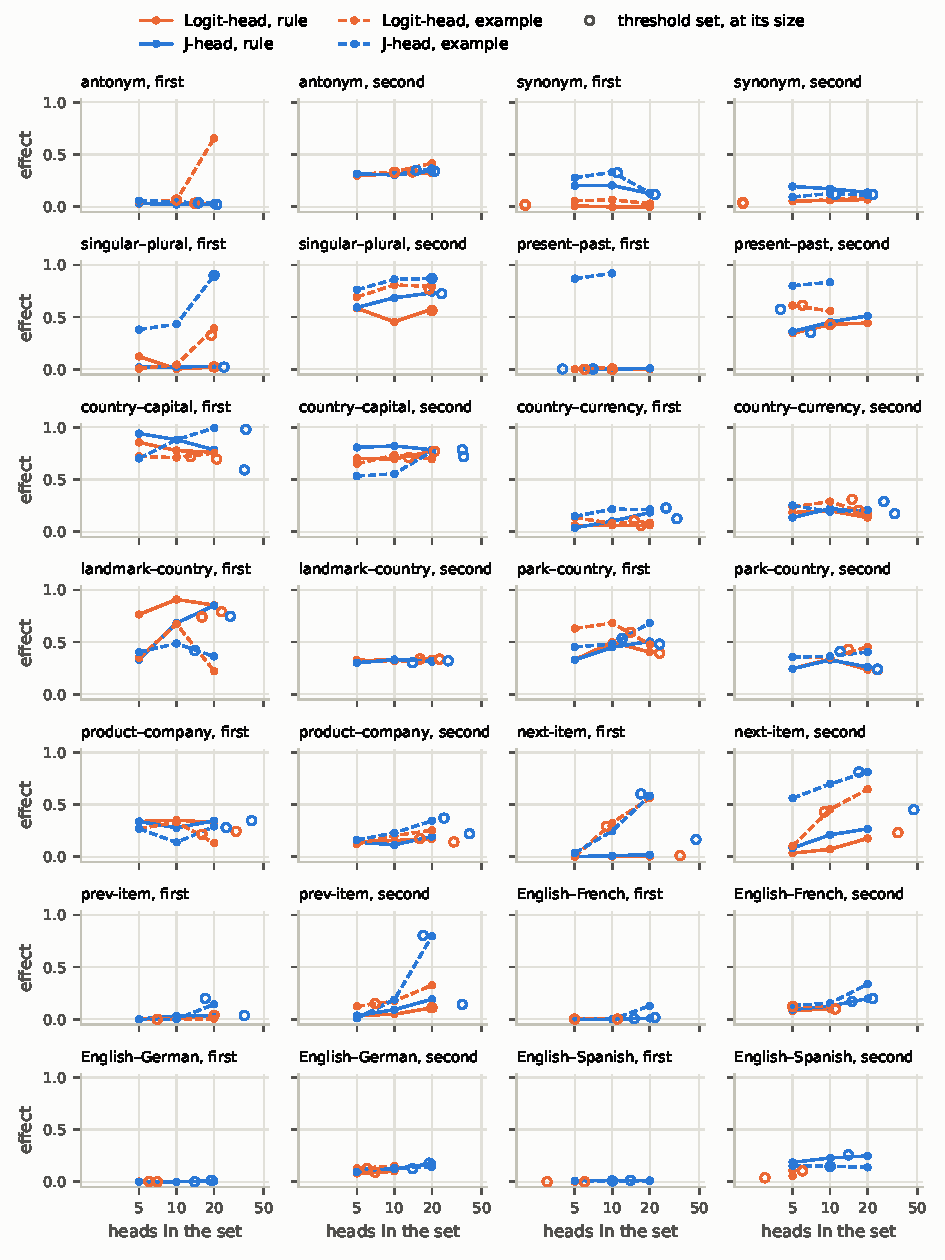
\includegraphics[width=\textwidth]{figures/sized_readouts.pdf}
\caption{Equal-size sets, E1 rule: causal effect against the number of heads (log scale), per task, in the first and the second check. Filled markers: sets of size 5, 10 and 20; hollow markers: the threshold set, at its own size. Solid: rule style; dashed: example style.}
\label{fig:sized-readouts}
\end{figure}

\begin{figure}[H]
\centering
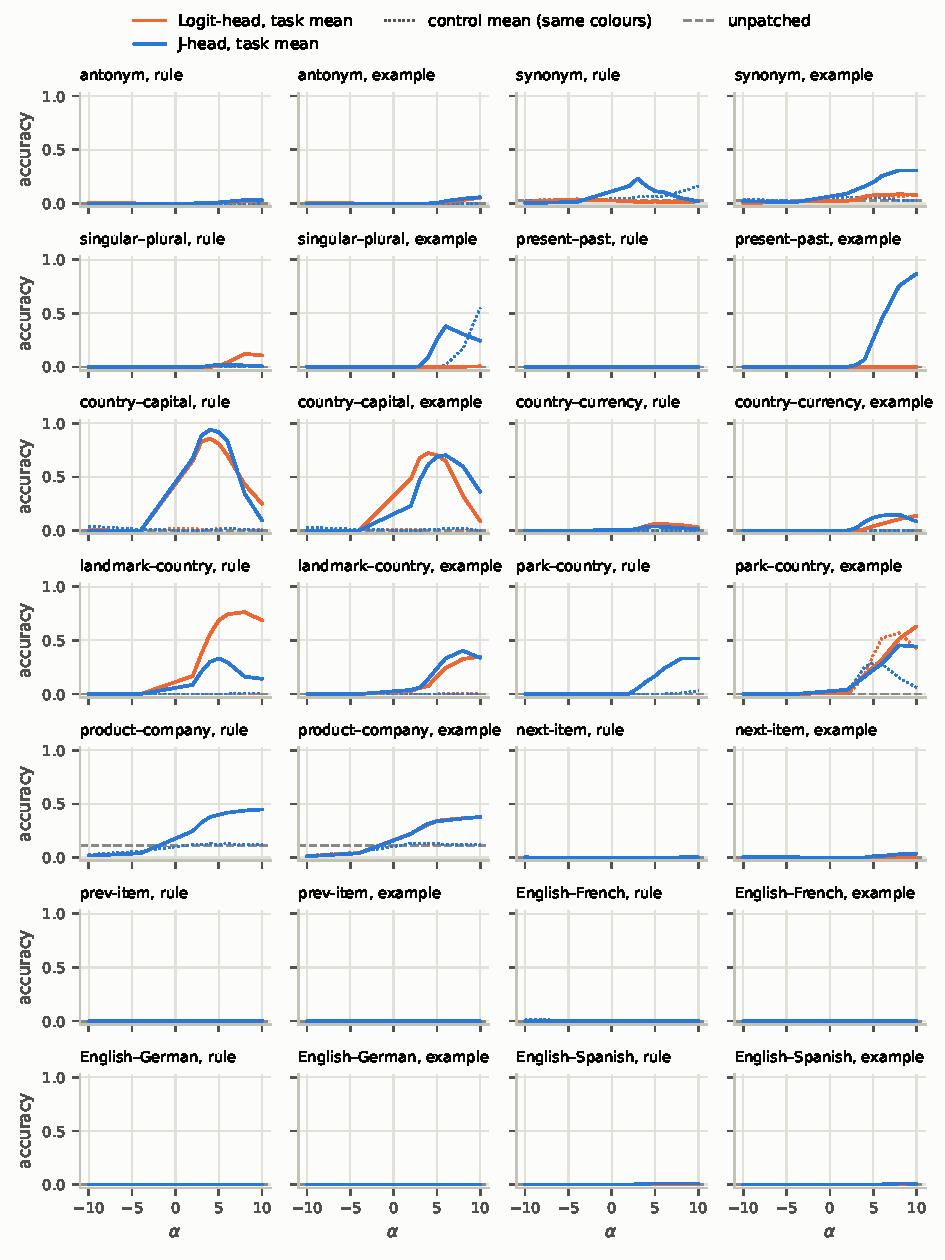
\includegraphics[width=\textwidth]{figures/sized_curves_n5.pdf}
\caption{Equal-size sets of the 5 highest-ranked heads under the rule of E1, first causal check: accuracy on the patched items against $\alpha$, with each style's set patched with means of the same style, averaged over the style's five source wordings, as Figure~\ref{fig:patch-simple}. Nine values of $\alpha$: $-10$, $-4$, and 2 to 10 (none between $-4$ and 2). Solid: the task mean; dotted: the control mean at the same heads; dashed: unpatched accuracy. Empty panel: fewer than 5 heads match on any prompt.}
\label{fig:sized-curves-n5}
\end{figure}

\begin{figure}[H]
\centering
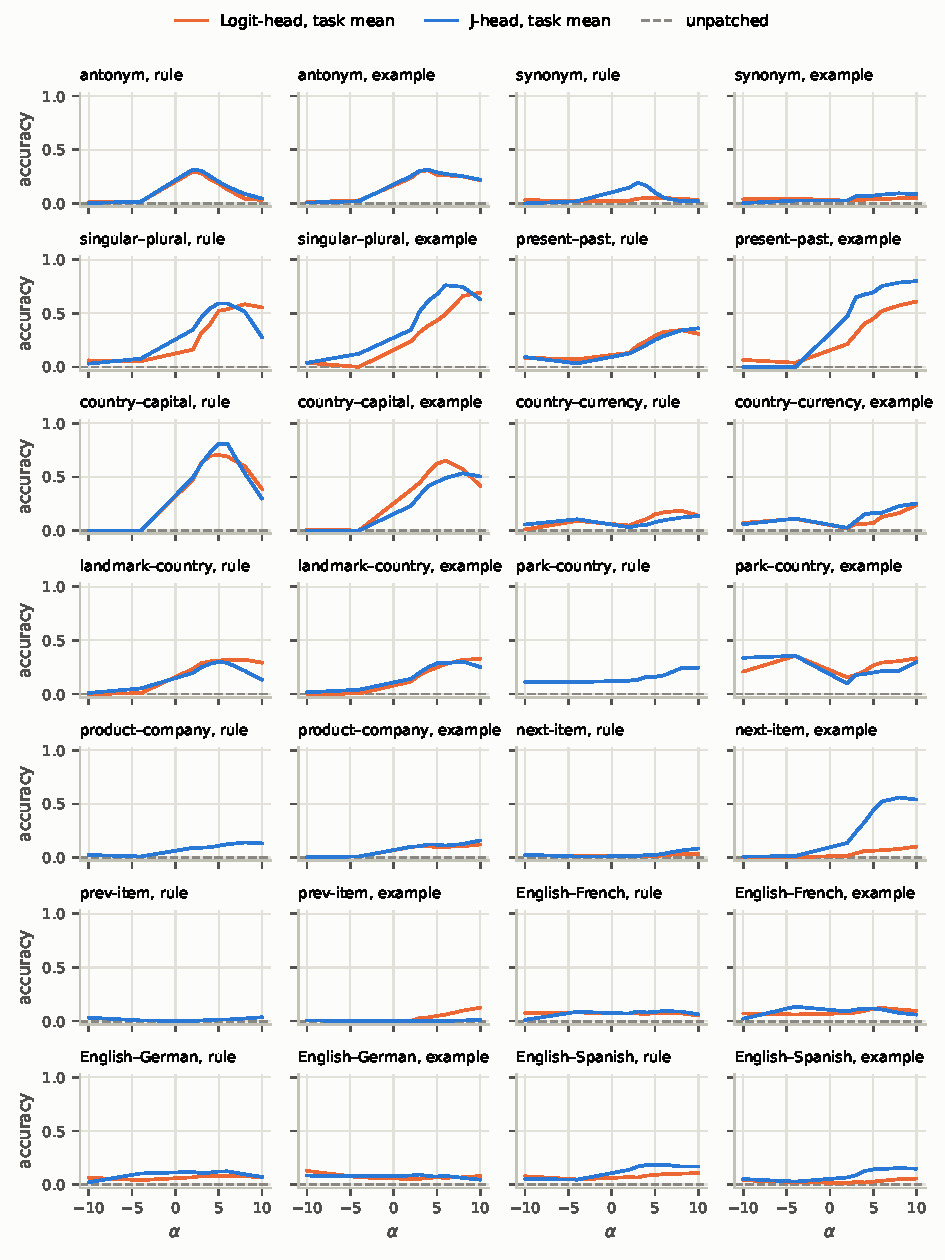
\includegraphics[width=\textwidth]{figures/sized_curves_n5_wrong.pdf}
\caption{Equal-size sets of 5 heads, E1 rule, second causal check, as Figure~\ref{fig:sized-curves-n5}, with the wrongly answered 1-shot prompts patched. No control mean.}
\label{fig:sized-curves-n5-wrong}
\end{figure}

\begin{figure}[H]
\centering
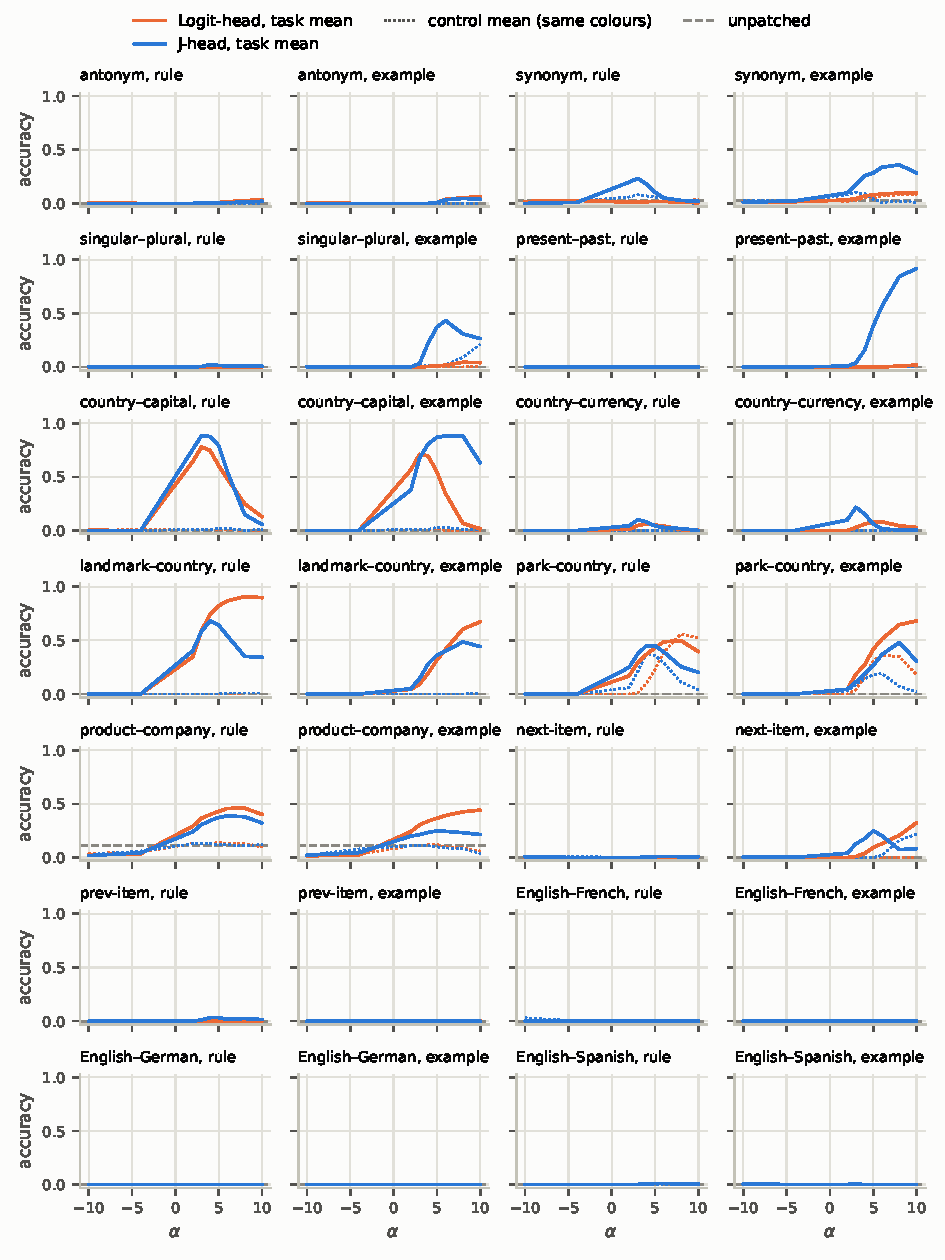
\includegraphics[width=\textwidth]{figures/sized_curves_n10.pdf}
\caption{Equal-size sets of 10 heads, E1 rule, first causal check, as Figure~\ref{fig:sized-curves-n5}.}
\label{fig:sized-curves-n10}
\end{figure}

\begin{figure}[H]
\centering
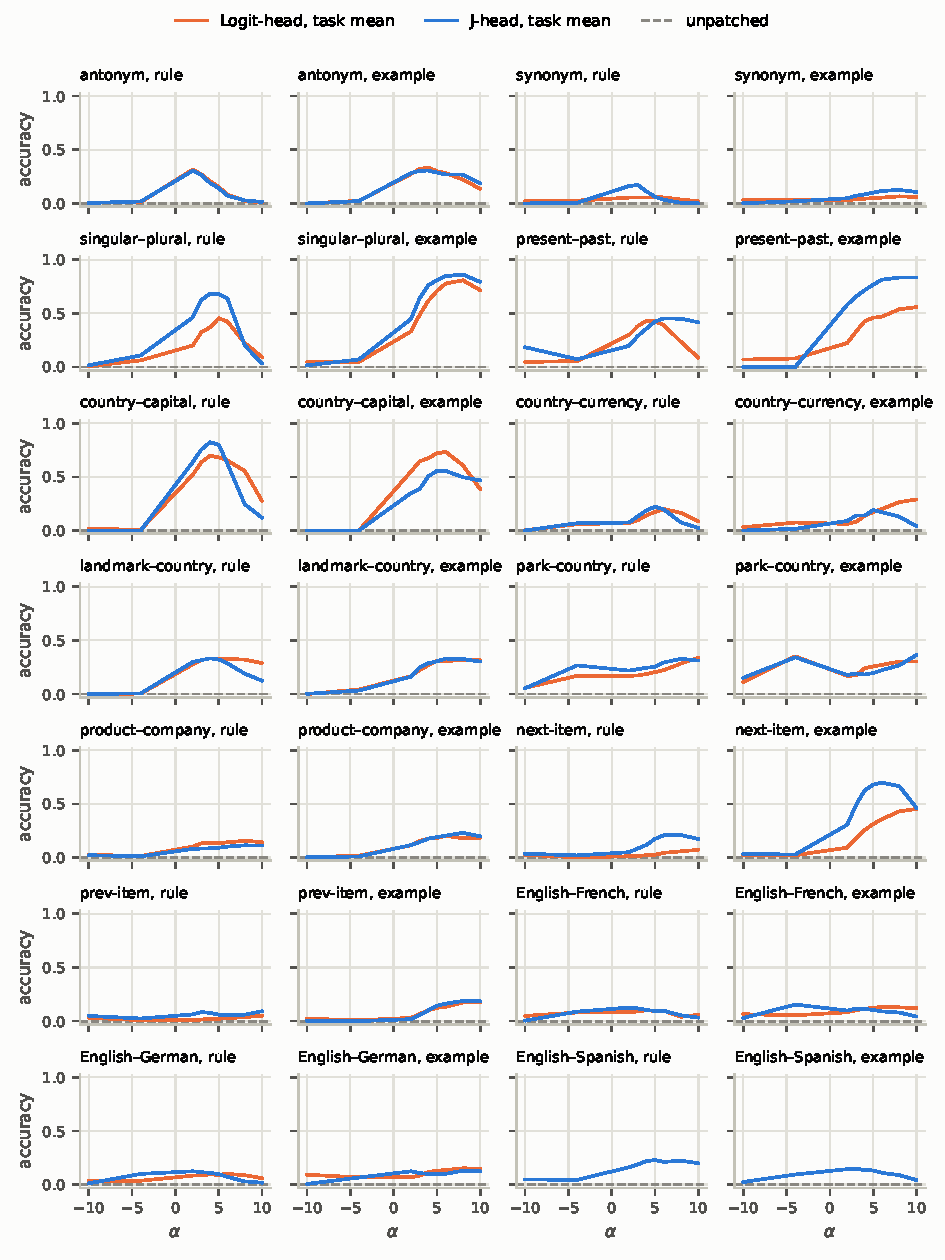
\includegraphics[width=\textwidth]{figures/sized_curves_n10_wrong.pdf}
\caption{Equal-size sets of 10 heads, E1 rule, second causal check, as Figure~\ref{fig:sized-curves-n5-wrong}.}
\label{fig:sized-curves-n10-wrong}
\end{figure}

\begin{figure}[H]
\centering
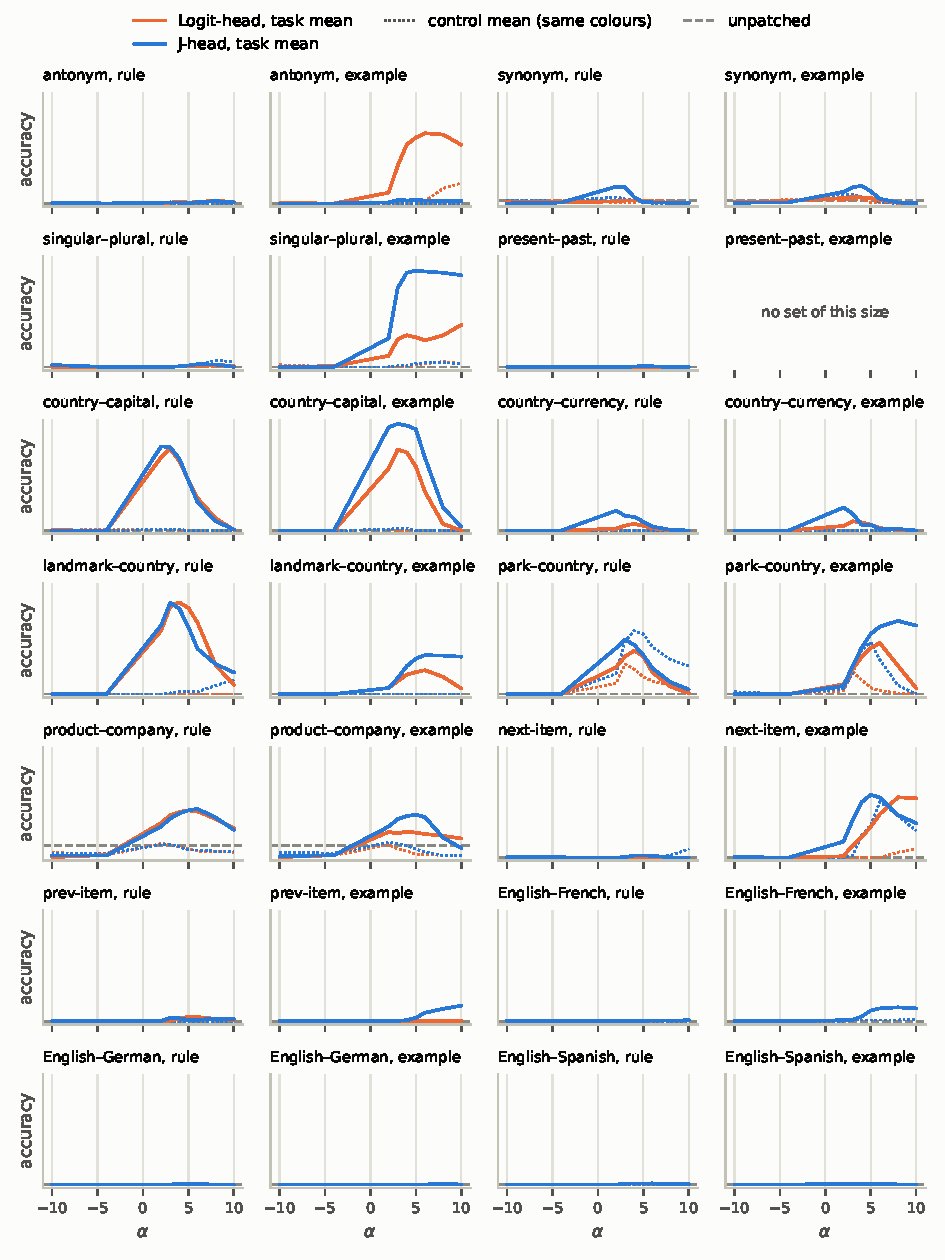
\includegraphics[width=\textwidth]{figures/sized_curves_n20.pdf}
\caption{Equal-size sets of 20 heads, E1 rule, first causal check, as Figure~\ref{fig:sized-curves-n5}.}
\label{fig:sized-curves-n20}
\end{figure}

\begin{figure}[H]
\centering
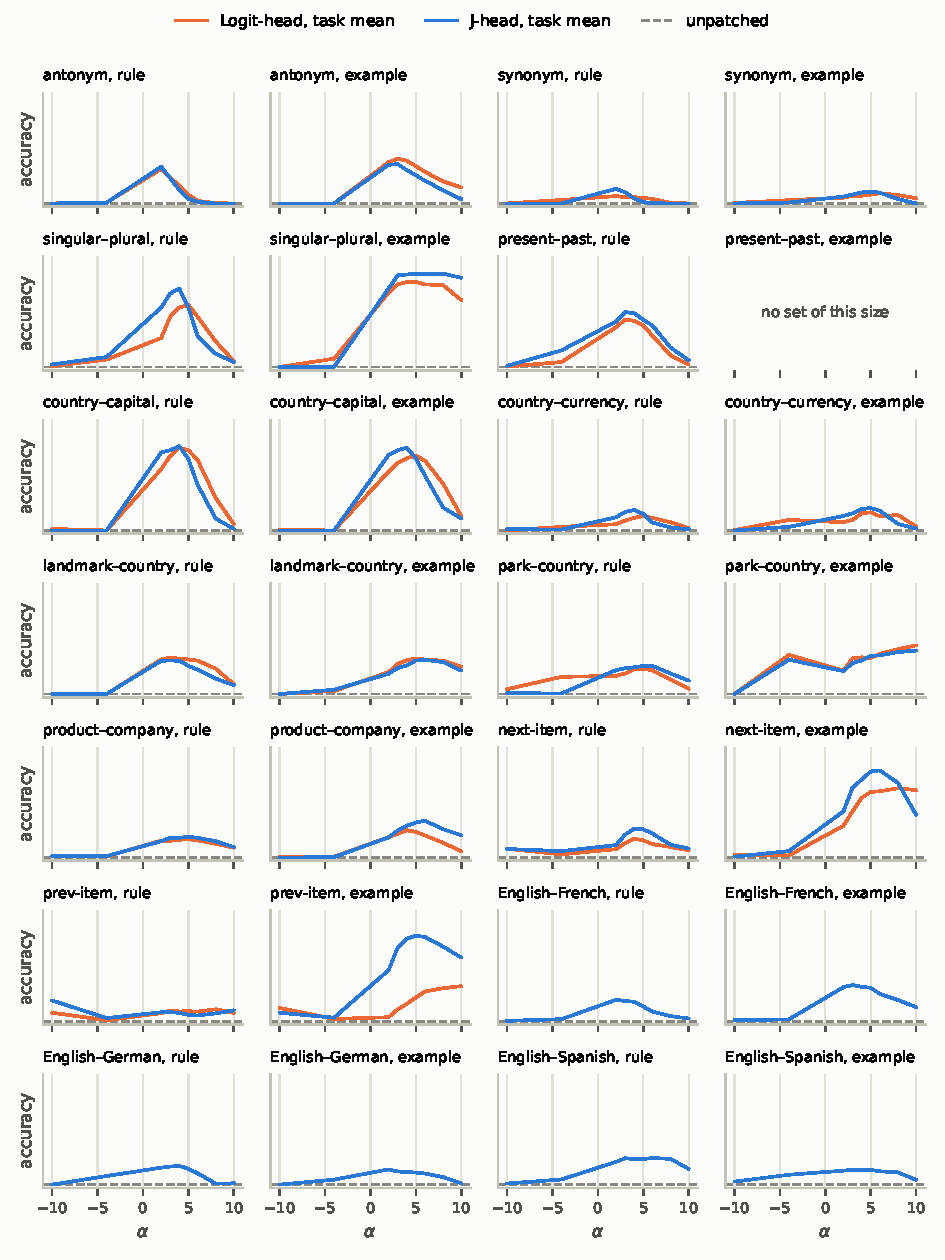
\includegraphics[width=\textwidth]{figures/sized_curves_n20_wrong.pdf}
\caption{Equal-size sets of 20 heads, E1 rule, second causal check, as Figure~\ref{fig:sized-curves-n5-wrong}.}
\label{fig:sized-curves-n20-wrong}
\end{figure}

\begin{figure}[H]
\centering
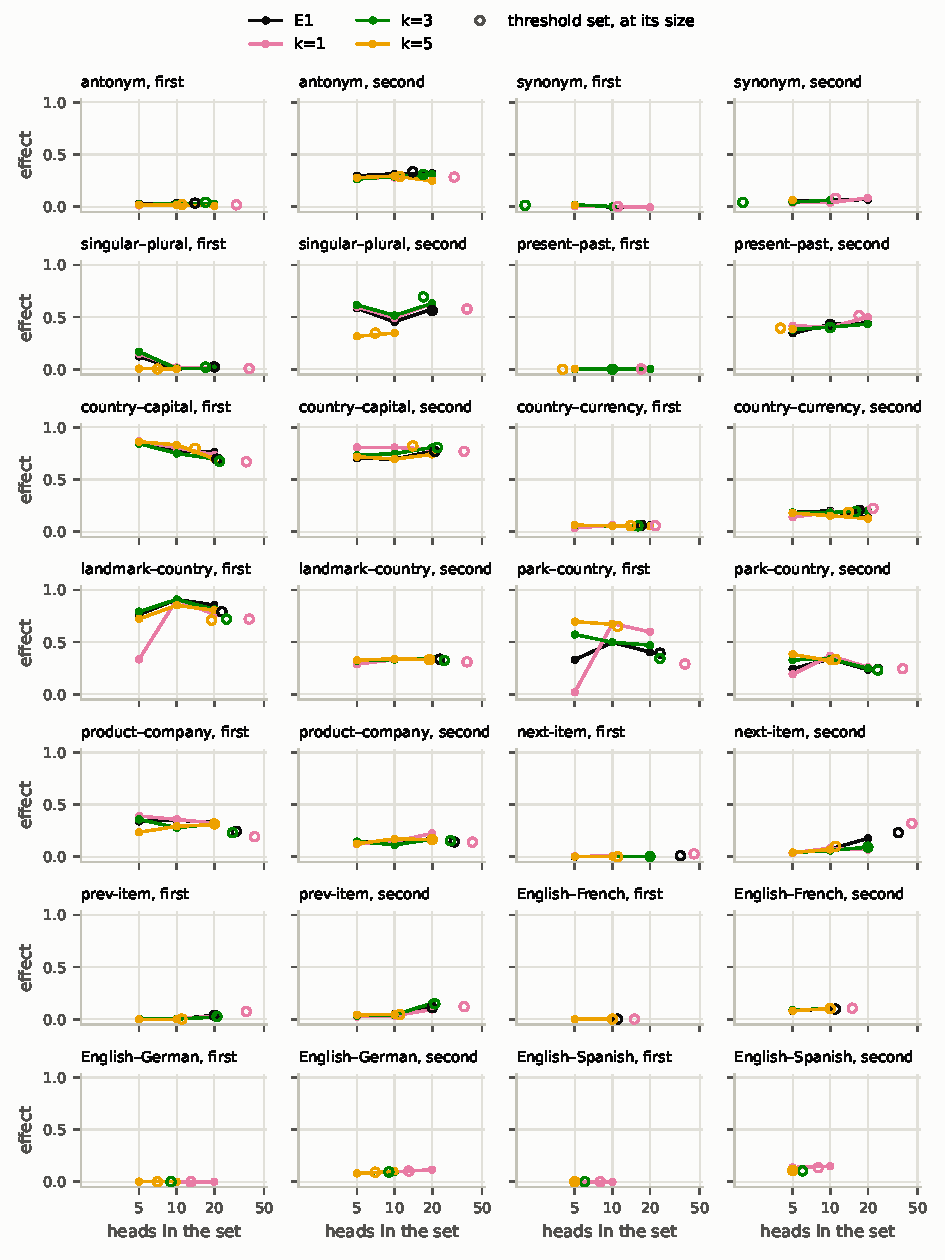
\includegraphics[width=\textwidth]{figures/sized_rules_logithead.pdf}
\caption{Equal-size sets, rule style, Logit-head: causal effect against the number of heads under the rule of E1 and the rules of E1b, as Figure~\ref{fig:sized-readouts}.}
\label{fig:sized-rules-logithead}
\end{figure}

\begin{figure}[H]
\centering
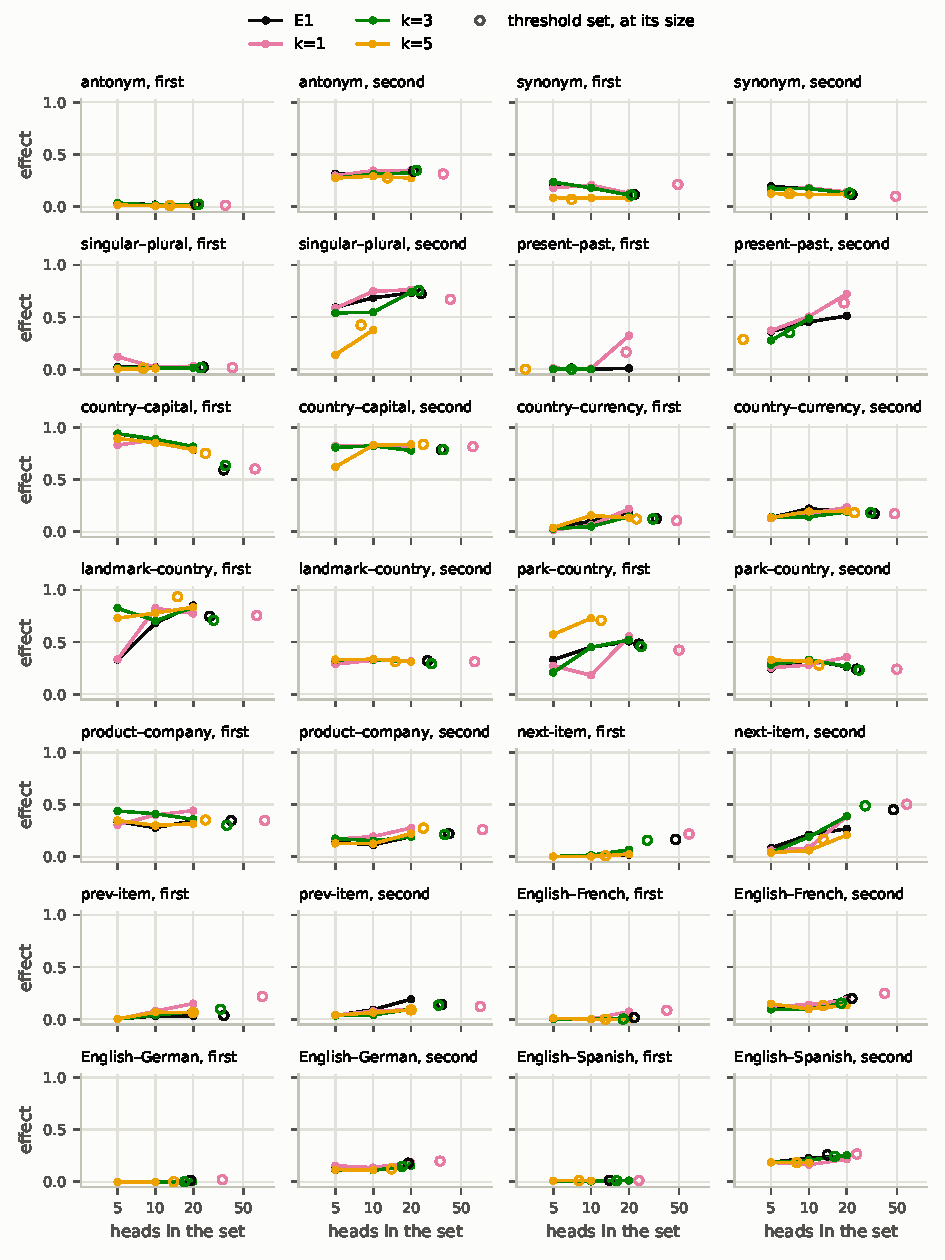
\includegraphics[width=\textwidth]{figures/sized_rules_jhead.pdf}
\caption{Equal-size sets, rule style, J-head, as Figure~\ref{fig:sized-rules-logithead}.}
\label{fig:sized-rules-jhead}
\end{figure}

\begin{figure}[H]
\centering
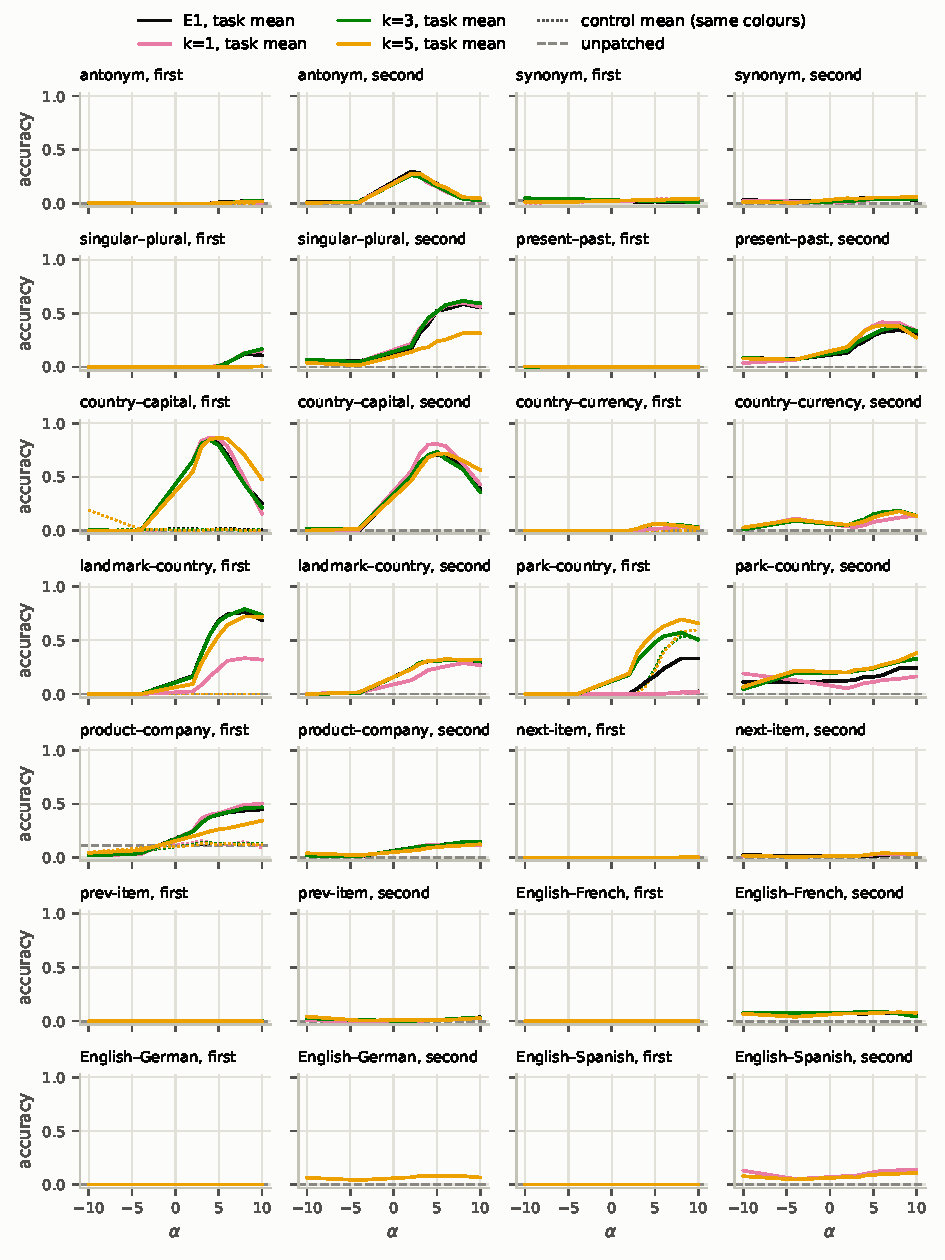
\includegraphics[width=\textwidth]{figures/sized_rule_curves_logithead_n5.pdf}
\caption{Equal-size sets of the 5 highest-ranked Logit-head heads, rule style, under the rule of E1 and the rules of E1b (at least $k$ of the five instruction templates): accuracy against $\alpha$ with rule-style means, averaged over the five templates, in the first check (with the control mean, dotted) and the second, as Figure~\ref{fig:patch-consensus}, at the nine values of $\alpha$ of Figure~\ref{fig:sized-curves-n5}. A missing curve: fewer than 5 heads match under that rule.}
\label{fig:sized-rule-curves-logithead-n5}
\end{figure}

\begin{figure}[H]
\centering
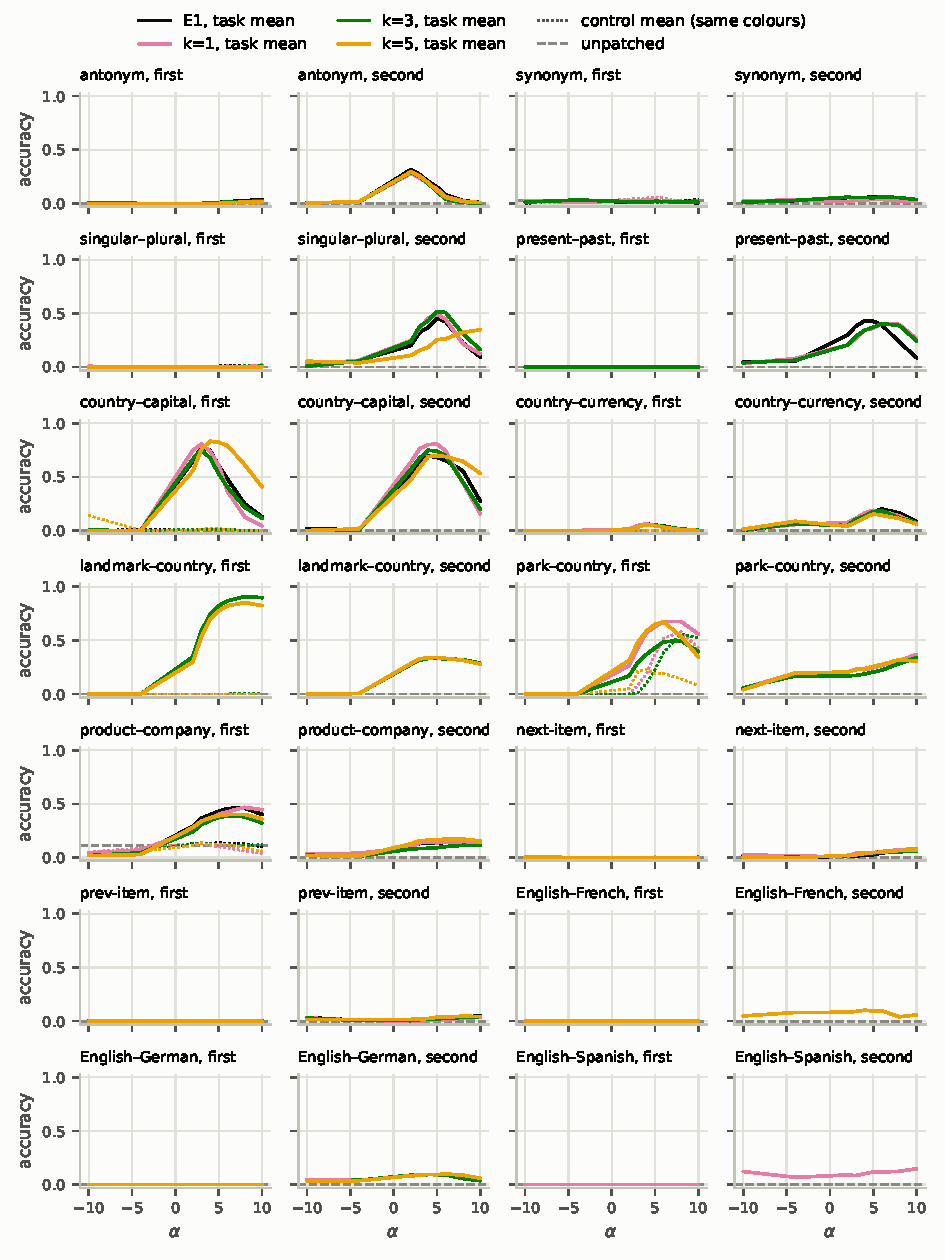
\includegraphics[width=\textwidth]{figures/sized_rule_curves_logithead_n10.pdf}
\caption{Equal-size sets of 10 Logit-head heads, rule style, E1 and E1b rules, as Figure~\ref{fig:sized-rule-curves-logithead-n5}.}
\label{fig:sized-rule-curves-logithead-n10}
\end{figure}

\begin{figure}[H]
\centering
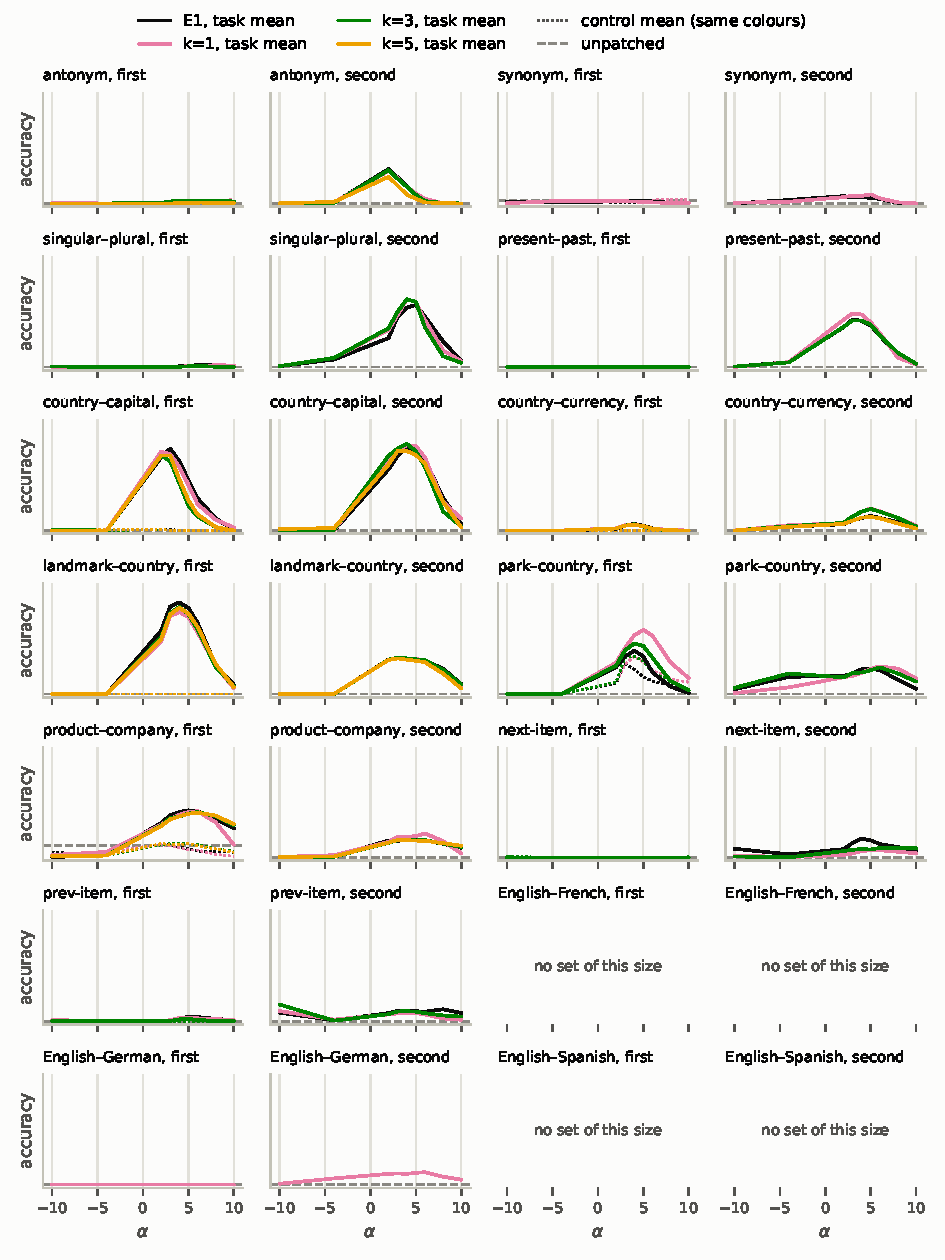
\includegraphics[width=\textwidth]{figures/sized_rule_curves_logithead_n20.pdf}
\caption{Equal-size sets of 20 Logit-head heads, rule style, E1 and E1b rules, as Figure~\ref{fig:sized-rule-curves-logithead-n5}.}
\label{fig:sized-rule-curves-logithead-n20}
\end{figure}

\begin{figure}[H]
\centering
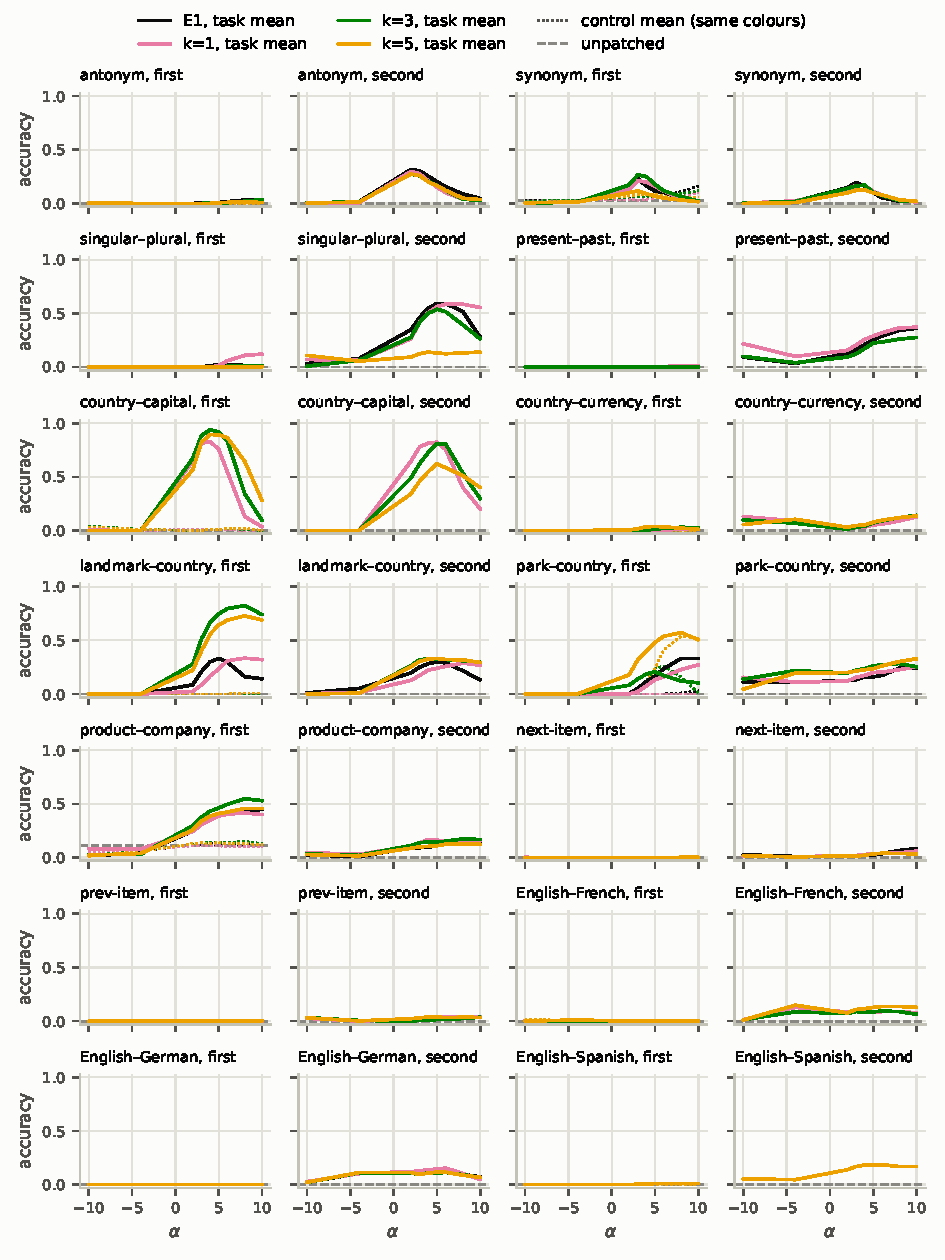
\includegraphics[width=\textwidth]{figures/sized_rule_curves_jhead_n5.pdf}
\caption{Equal-size sets of 5 J-head heads, rule style, E1 and E1b rules, as Figure~\ref{fig:sized-rule-curves-logithead-n5}.}
\label{fig:sized-rule-curves-jhead-n5}
\end{figure}

\begin{figure}[H]
\centering
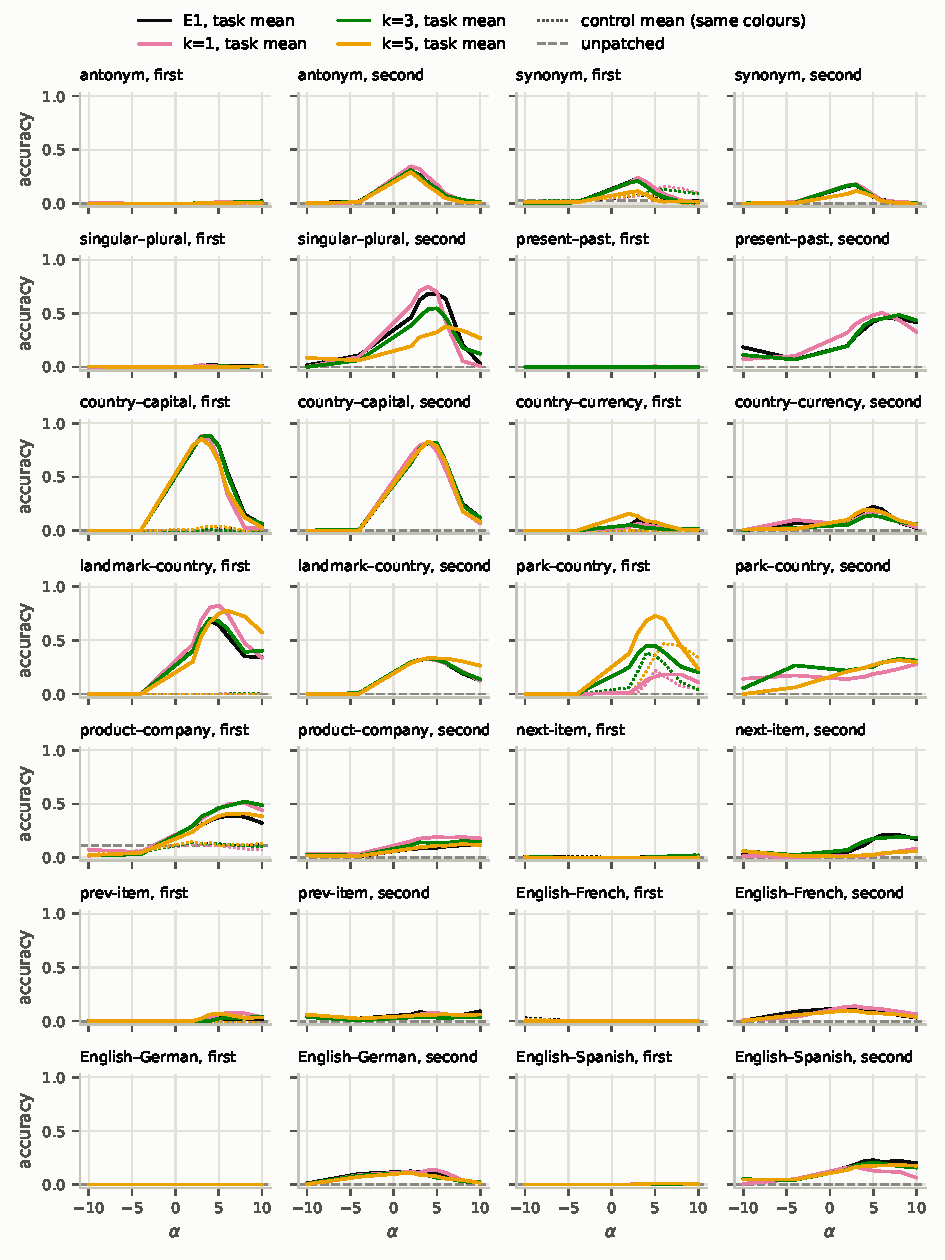
\includegraphics[width=\textwidth]{figures/sized_rule_curves_jhead_n10.pdf}
\caption{Equal-size sets of 10 J-head heads, rule style, E1 and E1b rules, as Figure~\ref{fig:sized-rule-curves-logithead-n5}.}
\label{fig:sized-rule-curves-jhead-n10}
\end{figure}

\begin{figure}[H]
\centering
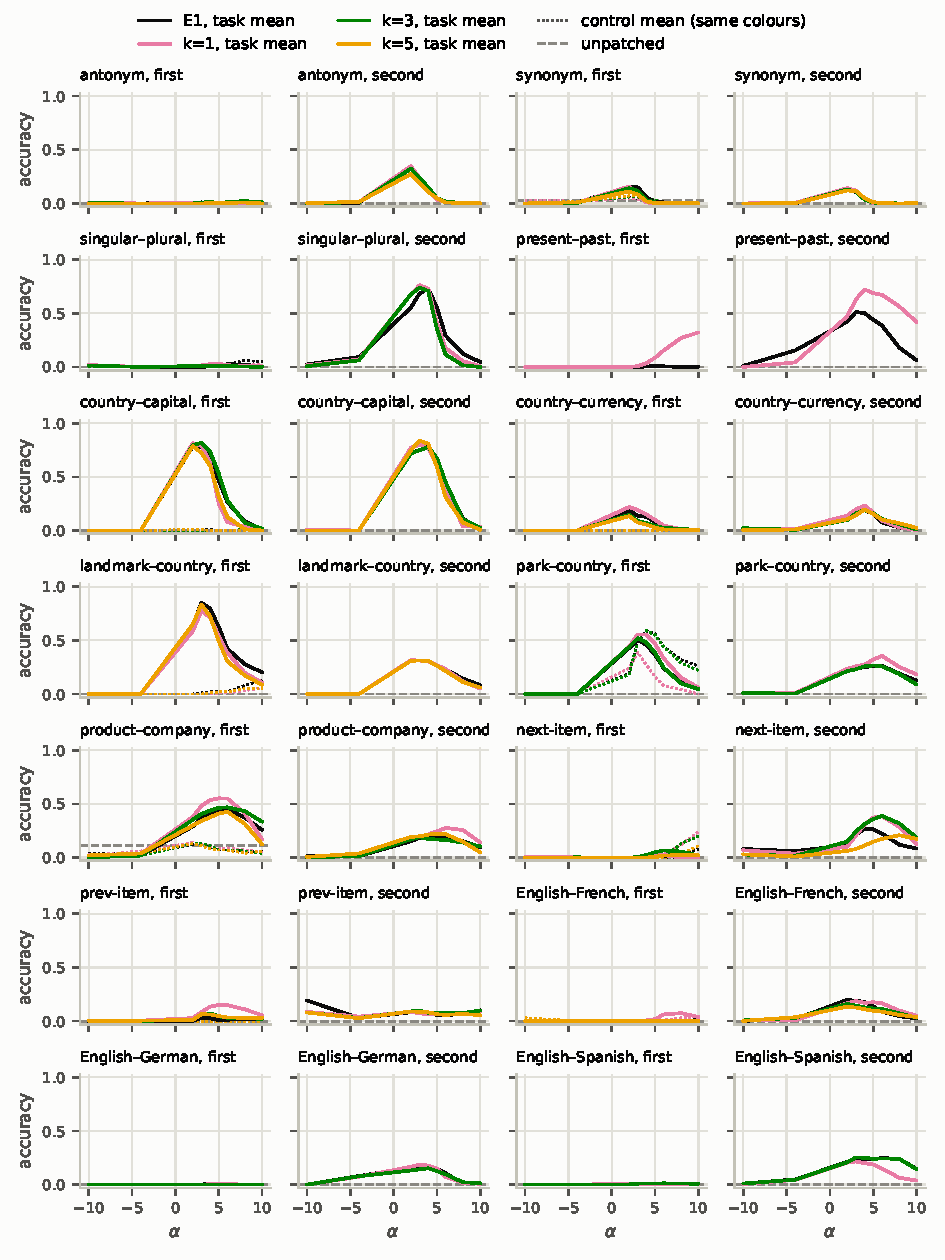
\includegraphics[width=\textwidth]{figures/sized_rule_curves_jhead_n20.pdf}
\caption{Equal-size sets of 20 J-head heads, rule style, E1 and E1b rules, as Figure~\ref{fig:sized-rule-curves-logithead-n5}.}
\label{fig:sized-rule-curves-jhead-n20}
\end{figure}

% =====================================================================
\section{Head sets from decoded words}\label{sec:words}
\subsection{Design}
\paragraph{Question.} The term lists of \citet{yang2026shared} are written by hand, and a head is selected if it decodes one of their words. The words the heads decode on a task's prompts may name the task differently: as the type of the answer (\emph{city} for country--capital), or with words that heads decode on every task. Do head sets chosen from the words the heads actually decode carry the task better than the E1 sets? And can a few heads be found that carry it alone? The question was asked after the results of the earlier sections; it has no hypothesis, and we report it as exploratory. Only J-head is used, and only the rule style.

\paragraph{Shared settings.} The J-head readings of E1: each head's ten top tokens at the last prompt token, on $P^{+}$ of each of the five instruction templates (at most 100 correct prompts each), pooled. Each head set is patched with the first causal check of E1, with the rule-style means of the five templates, averaged over them, and the control mean of E1, at four values of $\alpha$: 1, 2, 4 and 8, to shorten the runs. We report the highest accuracy over the four, and the E1 J-head rule-style sets over the same four. The second check is not run.

\paragraph{Words decoded.} Each top token is decoded, stripped of whitespace and lowercased, and kept as a word if it is alphabetic, has at least three letters, is not in a short list of function words, and is a common English word (Zipf frequency at least 3 in \texttt{wordfreq}). A word's \emph{share} on a task is the fraction of pairs of prompt and head, over all 1{,}024 heads and the pooled prompts, whose ten top tokens contain it. \emph{Task words}: the words with the largest share on the task minus their mean share on the other 13 tasks. \emph{Common words}: the words with the largest minimum share over the 14 tasks.

\paragraph{CC-pooled.} The list of a task is its 5 top task words and the 5 top common words, turned into token ids as Yang's lists are (Definition~\ref{def:lth}: case variants, leading space). Heads are selected with Definition~\ref{def:lth} ($k=10$, $\rho=0.1$) on the five templates' prompts pooled, about 500 per task, rather than on the most accurate template.

\paragraph{CC-pooled-clean.} Following \citet{davidson2025different}, who contrast task prompts with unrelated text, every head is also read on 1{,}000 passages of WikiText-103, cut to the token lengths of the rule prompts. The 50 words with the largest share there are removed before the task and common words are chosen; heads are then selected as for CC-pooled. Lists of 5 + 5 and 10 + 10 words.

\paragraph{Attend and decode.} At the last prompt token, head L16H25 attends to the words \emph{capital} and \emph{country} of the instruction and decodes \emph{city}. To find heads with this pattern, the task words of a task are the alphabetic words of Yang's term list and its 10 top task words. A head's \emph{attention} is its share of the last token's attention on the tokens of these words in the prompt, outside the input $x$, averaged over the pooled prompts (eager attention, each prompt run alone). Its \emph{decode rate} is the share of the same prompts whose ten top J-head tokens contain a token of these words. Heads are ranked by the product of the two, and the first $N\in\{1,2,3,5,10,20\}$ are patched.

\paragraph{Random sets.} For the sets of 5 and 10 heads, two random sets with the same number of heads in each layer, drawn outside the set.

\begin{sloppypar}\paragraph{Output.} \texttt{results/word\_lists\_union} (CC-pooled), \texttt{results/neutral\_union} (CC-pooled-clean), \texttt{results/attend\_decode}; WikiText readings in \texttt{data/readings/neutral}, attention masses in \texttt{data/readings/attention\_rule}. Other designs tried along the way (word lists from one template, other list lengths, strict consensus, other contrasts, ranking by match rate) are listed in \texttt{summary-simple}.\end{sloppypar}

\subsection{Results}\label{sec:res-words}
\paragraph{CC-pooled} (Table~\ref{tab:words}). The CC-pooled set has a larger effect than the E1 set on every task, and it carries several tasks on which the E1 set has none: antonym, singular--plural, next-item and the three translation tasks. Present--past stays near the baseline under every set of this section but one (below). Each part of the design matters: lists of task words alone or common words alone, and heads selected on the most accurate template only, give smaller effects (\texttt{summary-simple}). The sets have 95 to 137 heads. Random sets of the same size, with the same heads per layer, have almost no effect on most tasks, but single draws have large effects on antonym and landmark--country, and every draw has some on product--company. The control mean has effects on synonym, and smaller ones on park--country, singular--plural and next-item (Table~\ref{tab:words-control}), so on these tasks part of the effect is not specific to the task.

\paragraph{CC-pooled-clean.} The common words of CC-pooled (\emph{what}, \emph{which}, \emph{maybe}, \emph{https}, \emph{etc}) are among the words heads decode on unrelated text. Removing them helps most fact tasks, the translation tasks and the morphology tasks (with 10 + 10 words it is the only set with some effect on present--past), and hurts antonym, synonym, next-item and prev-item, which are carried by heads that decode such generic words.

\paragraph{Attend and decode.} For tasks whose instruction names the type of the answer, a few heads carry the task. L16H25 ranks first on all five fact tasks; alone it has the largest effect of all sets on country--capital, five heads carry landmark--country, and twenty carry product--company and singular--plural as much as or more than CC-pooled, with no effect of the control mean. On park--country the control mean has an effect almost as large. Translations, next-item, prev-item and present--past are not carried by up to twenty such heads, although the translation tasks have heads with this pattern. The heads with the pattern lie mostly in layers 13 to 17. At equal size, the sets ranked this way have larger effects on average than the CC-pooled heads ranked by match rate, and random sets have almost none, with single draws on singular--plural and product--company the exceptions.

\paragraph{Caveats.} The word lists, list sizes and designs were chosen after seeing the first check on the same items, the effect is the best over four values of $\alpha$, each set is run once, and the second check and held-out items have not been run here; both are run in E4 (Sec.~\ref{sec:e4}).

Thus, lists built from the words the heads decode select head sets that carry more tasks than Yang's term lists, and for tasks whose instruction names the answer type, heads that attend to that name and decode the type of the answer carry the task with one to twenty heads.

\begin{table}[H]
\centering\footnotesize\setlength{\tabcolsep}{4pt}
% Generated by scripts/e3/wordlist_tables.py from results/.
\begin{tabular}{lrrrrrrrr}
\toprule
Task & unpatched & E1 & CC-pooled & CC-pooled-clean & A+D 1 & A+D 5 & A+D 20 & random 5 \\
\midrule
antonym & 0.00 & 0.02 & \textbf{0.54} & 0.16 & 0.01 & 0.25 & 0.16 & 0.06 \\
synonym & 0.03 & 0.15 & \textbf{0.42} & 0.12 & 0.09 & 0.11 & 0.16 & 0.04 \\
singular--plural & 0.00 & 0.01 & 0.64 & 0.57 & 0.00 & 0.08 & \textbf{0.68} & 0.21 \\
present--past & 0.00 & 0.00 & 0.03 & 0.02 & 0.00 & 0.00 & \textbf{0.04} & 0.00 \\
country--capital & 0.00 & 0.59 & 0.73 & 0.73 & \textbf{0.88} & 0.76 & 0.72 & 0.02 \\
country--currency & 0.00 & 0.12 & 0.29 & \textbf{0.38} & 0.00 & 0.04 & 0.23 & 0.00 \\
landmark--country & 0.00 & 0.69 & 0.92 & \textbf{0.97} & 0.70 & 0.79 & 0.43 & 0.05 \\
park--country & 0.00 & 0.44 & \textbf{0.76} & 0.68 & 0.42 & 0.36 & 0.19 & 0.06 \\
product--company & 0.11 & 0.46 & 0.52 & 0.66 & 0.33 & 0.48 & \textbf{0.72} & 0.12 \\
next-item & 0.00 & 0.17 & \textbf{0.43} & 0.04 & 0.00 & 0.01 & 0.01 & 0.00 \\
prev-item & 0.00 & 0.02 & \textbf{0.18} & 0.08 & 0.00 & 0.03 & 0.03 & 0.00 \\
English--French & 0.00 & 0.01 & 0.25 & \textbf{0.40} & 0.00 & 0.00 & 0.02 & 0.01 \\
English--German & 0.00 & 0.01 & \textbf{0.32} & 0.30 & 0.00 & 0.00 & 0.08 & 0.00 \\
English--Spanish & 0.00 & 0.01 & \textbf{0.30} & 0.17 & 0.01 & 0.01 & 0.03 & 0.00 \\
\midrule
mean & 0.01 & 0.19 & 0.45 & 0.38 & 0.17 & 0.21 & 0.25 & 0.04 \\
\bottomrule
\end{tabular}

\caption{Head sets from decoded words, J-head, rule style, first causal check: highest accuracy over $\alpha\in\{1,2,4,8\}$, rule-style means averaged over the five templates. E1: E1's J-head rule-style set over the same $\alpha$. A+D $N$: the $N$ heads ranked first by attention to task words times decode rate. Random 5: mean of the two layer-matched random sets of A+D 5. Bold: the largest of the six head sets.}
\label{tab:words}
\end{table}

\begin{table}[H]
\centering\footnotesize\setlength{\tabcolsep}{4pt}
% Generated by wordlist_tables.py (session scratchpad) from results/.
\begin{tabular}{lrrrrrrrr}
\toprule
Task & unpatched & E1 & CC-pooled & CC-pooled-clean & A+D 1 & A+D 5 & A+D 20 & random 5 \\
\midrule
antonym & 0.00 & 0.00 & 0.00 & 0.00 & 0.00 & 0.00 & 0.00 & 0.00 \\
synonym & 0.03 & 0.05 & 0.26 & 0.09 & 0.07 & 0.03 & 0.05 & 0.03 \\
singular--plural & 0.00 & 0.00 & 0.12 & 0.03 & 0.00 & 0.00 & 0.00 & 0.01 \\
present--past & 0.00 & 0.00 & 0.01 & 0.00 & 0.00 & 0.00 & 0.00 & 0.00 \\
country--capital & 0.00 & 0.00 & 0.00 & 0.00 & 0.00 & 0.00 & 0.00 & 0.01 \\
country--currency & 0.00 & 0.00 & 0.00 & 0.00 & 0.00 & 0.00 & 0.00 & 0.00 \\
landmark--country & 0.00 & 0.00 & 0.05 & 0.01 & 0.00 & 0.00 & 0.00 & 0.04 \\
park--country & 0.00 & 0.18 & 0.17 & 0.11 & 0.35 & 0.20 & 0.13 & 0.01 \\
product--company & 0.11 & 0.08 & 0.08 & 0.07 & 0.12 & 0.13 & 0.09 & 0.15 \\
next-item & 0.00 & 0.12 & 0.12 & 0.00 & 0.00 & 0.00 & 0.00 & 0.00 \\
prev-item & 0.00 & 0.00 & 0.01 & 0.00 & 0.00 & 0.00 & 0.00 & 0.00 \\
English--French & 0.00 & 0.00 & 0.05 & 0.05 & 0.00 & 0.00 & 0.00 & 0.00 \\
English--German & 0.00 & 0.00 & 0.01 & 0.01 & 0.00 & 0.00 & 0.00 & 0.00 \\
English--Spanish & 0.00 & 0.00 & 0.01 & 0.01 & 0.00 & 0.00 & 0.00 & 0.00 \\
\midrule
mean & 0.01 & 0.03 & 0.06 & 0.03 & 0.04 & 0.03 & 0.02 & 0.02 \\
\bottomrule
\end{tabular}

\caption{As Table~\ref{tab:words}, with the control mean, at the $\alpha$ of the highest task-mean accuracy.}
\label{tab:words-control}
\end{table}

% =====================================================================
\section{E4: Held-out test of head sets from decoded words}
\label{sec:e4}

\subsection{Design}

\paragraph{Question.} In Sec.~\ref{sec:words} the head sets chosen from the words heads decode
(CC-pooled) carry every task better than the E1 J-head sets, and carry tasks the E1 sets do
not (antonym, singular--plural, next-item, the three translations). That result is exploratory:
the words, the list sizes and the designs were chosen after seeing the first check on the same
items, each effect is the best of four values of $\alpha$, each set was run once, the second check
was not run, and the sets (95 to 137 heads) are larger than the E1 sets and than the function
vector of \citet{davidson2025different}. E4 asks three questions with the design of Sec.~\ref{sec:words} frozen:
(i) does CC-pooled still beat the E1 set on items not used to build it; (ii) is its effect larger
than that of random heads of the same number and layers; (iii) at the same number of heads, do
heads chosen by what they decode carry the task as well as heads chosen by their causal effect
\citep{davidson2025different}? A second part, E4b (Sec.~\ref{sec:e4b}), adds new wordings of
each task's instruction and asks two more: (iv) do words and heads chosen on more wordings
carry the task better; (v) do heads chosen on some wordings carry the task when it is asked in
wordings never used to choose them? The hypotheses are stated before the run (below).

\paragraph{Frozen choices.} Everything that Sec.~\ref{sec:words} chose after seeing results is fixed here
and not changed after E4 is run: J-head readout; rule style; word filter (alphabetic, at least
three letters, not a function word, Zipf frequency at least 3); task words by share on the task
minus the mean share on the other 13 tasks; common words by the largest minimum share over
the 14 tasks; 5 task words and 5 common words; heads by Definition~\ref{def:lth} with $k = 10$,
$\rho = 0.10$, on the five templates' prompts pooled; for CC-pooled-clean the 50 words with the
largest share on the 1{,}000 WikiText-103 passages removed first; for attend and decode the
score of Sec.~\ref{sec:words}. No other list, list size, threshold or contrast is run in E4.

\paragraph{Item split.} The items of each task are shuffled with a fixed seed (0) and cut into
two halves, $A$ and $B$, of equal size (one more in $A$ when odd). Each half is used once to
choose and once to test (two folds): in fold~1 everything is chosen on $A$ and tested on $B$;
in fold~2 the reverse. ``Chosen'' covers every quantity that depends on the items: the
identification prompts $P^+$ of each template (the first 100 correct prompts of that half),
the word shares, the word lists, the head sets, the rankings of the top-$N$ sets, the
function-vector scores, the task means and the control means (the control task's own half
with the same name). ``Tested'' covers only the patched items. The WikiText readings do not
depend on the items and are shared by both folds. On tasks with fewer than 200 items a half
gives fewer than 100 identification prompts or patched items; the number used is reported for
every task, fold and check.

\paragraph{Head sets.} For each task and fold, all J-head:
\begin{enumerate}
  \item \textbf{E1}: Definition~\ref{def:lth} with Yang et al.'s term list on the most accurate template
    of the choosing half (the E1 rule, recomputed on that half).
  \item \textbf{CC}: CC-pooled at its own size $N_t$ (the heads passing Definition~\ref{def:lth}).
  \item \textbf{CC-20, CC-40}: the first 20 and 40 heads of the model ranked by their pooled
    match rate under the CC list (ties as in Sec.~\ref{sec:sized}); a head need not pass the threshold.
  \item \textbf{FV-$N$}, $N \in \{20, 40, N_t\}$: the first $N$ heads ranked by the
    function-vector score of \citet{davidson2025different} on task $t$ (the gain in the answer's
    probability when the head is set to its mean on prompts whose instruction is replaced, as
    run for \texttt{summary-simple}), computed on the choosing half only.
  \item \textbf{Random-$N$}, $N \in \{20, 40, N_t\}$: five draws per size, each with the same
    number of heads in every layer as the CC set of that size, drawn outside it (seeds 0--4).
  \item Secondary, not in the hypotheses: \textbf{CC-clean} (5\,+\,5 words, pooled), and
    \textbf{A+D-20, A+D-40} (attend and decode); \textbf{FV-univ-20, FV-univ-40}, the heads
    ranked by the mean of the function-vector score over the 14 tasks (Davidson et al.'s own
    choice of heads).
\end{enumerate}
The FV ranking uses a causal criterion on prompts without the instruction, close to the first
check itself; the comparison is therefore tilted towards the FV heads, not against them.

\paragraph{Causal checks.} Both checks of E1 (Sec.~\ref{sec:e1}), on the testing half, with the
rule-style means of the five templates of the choosing half and the control mean of E1's
control task, at ten values of $\alpha$: the nine of Sec.~\ref{sec:sized} ($-10, -4, 2, 3, 4, 5, 6, 8, 10$),
which give within 0.05 of the fifteen on the E1 and E1b sets, and $\alpha = 1$, added because
the CC sets of Sec.~\ref{sec:words} had their best effect at $\alpha \le 2$ on 11 of the 14 tasks. Check~1: the first 100 items of
the testing half answered correctly with one shot, patched in their zero-shot prompts. Check~2:
the first 100 answered wrongly with one shot, patched in their 1-shot prompts; unlike E1, the
control mean is run in check~2 as well. Random sets are patched with the task means only.
Scoring: the flexible score; the first-token score and the reply kinds of Sec.~\ref{sec:replies} are kept beside
it. As a reference, not a matched comparison, Davidson et al.'s own intervention (the 30-head
function vector of \texttt{summary-simple}, the sum of its heads' means added after layer 11 at the last
token, $\alpha = 1$) is run on the
same items.

\paragraph{Choice of $\alpha$.} Two effects are reported for every set, check and task. The
\emph{best-$\alpha$ effect}, as in the earlier sections: the highest accuracy over the ten
values, averaged over the five means, minus the unpatched accuracy. The \emph{cross-fitted
effect}, the primary measure: for fold~1, the accuracy at the $\alpha$ that gave the highest
accuracy for the same task and the same kind of set (same rule, same $N$) in fold~2, and the
reverse; the
choice of $\alpha$ is therefore never made on the items it is scored on. Random sets are scored
at the $\alpha$ chosen for the CC set of their size. Effects are averaged over the two folds.
The \emph{specific effect} is the task-mean accuracy minus the control-mean accuracy at the
same $\alpha$.

\paragraph{Statistics.} Two sets of the same task are patched on the same items, so they are
compared item by item. Each difference between two sets (on one task, or averaged over the 14
tasks) gets a 95\% interval from a paired bootstrap over the patched items within each task
(10{,}000 resamples, both folds resampled separately). The cross-fitted $\alpha$ is held fixed
in the resamples. A task counts for a set in the
per-task counts below only if the set's control effect is less than half of its effect on that
task.

\paragraph{Hypotheses.} All on the cross-fitted effect in check~1; the same comparisons in
check~2 are reported as secondary.
\begin{description}
  \item[H4 (lexicon).] CC has a larger effect than E1. Supported if the mean difference over
    the 14 tasks has a 95\% interval above 0 and CC is above E1 on at least 10 of the 14 tasks.
    Falsified if the interval contains 0 or CC is above E1 on 7 tasks or fewer.
  \item[H5 (not chance).] CC has a larger effect than random heads of its size and layers.
    Supported if its mean over the 14 tasks is above that of every random draw and, on at
    least 10 tasks, above the largest of the five draws. Falsified if its mean falls within the
    range of the five draws' means.
  \item[H6 (decoding against causal choice).] At each size $N \in \{20, 40, N_t\}$, CC-$N$
    is not worse than FV-$N$: the lower end of the 95\% interval of the mean difference
    (CC-$N$ minus FV-$N$) is above $-0.05$. In addition, CC-$N$ is above FV-$N$ on at least
    4 of the 5 tasks on which the E1 sets do nothing and the CC set did most in Sec.~\ref{sec:words}:
    antonym, next-item, English--French, English--German, English--Spanish. Decided
    separately for each $N$; falsified at a size if either part fails.
\end{description}
Expected from the earlier results, and stated so that the outcome can be compared with it:
H4 and H5 hold; H6 holds at $N_t$ and may fail at 20 and 40, where CC sets ranked by match
rate gave 0.21 and 0.25 (\texttt{summary-simple}, E3) and the 30-head FV of \texttt{summary-simple} has a larger mean.

\paragraph{What each outcome would mean.}
\begin{itemize}
  \item H4 and H5 hold, H6 holds at every $N$: choosing heads by what they decode is as
    good as choosing them by their causal effect, and better on the tasks named in H6. This
    is the strongest outcome, and the one that would make Sec.~\ref{sec:words} a main result.
  \item H4 and H5 hold, H6 only at $N_t$: decoded words find the right heads, but spread
    over more of them than a causal ranking needs; the claim becomes one about which heads,
    not how few.
  \item H4 holds, H5 fails: the CC sets work by their size and layers, not by which heads
    they hold; Sec.~\ref{sec:words}'s gain over E1 is a size effect.
  \item H4 fails: Sec.~\ref{sec:words}'s gain came from choosing the design on the test items.
\end{itemize}

\subsection{Results}\label{sec:res-e4}
\paragraph{What is reported.} Accuracies only: at the cross-fitted $\alpha$, averaged over the two folds (Tables~\ref{tab:e4-check1}--\ref{tab:e4-secondary}), and against $\alpha$ (Figure~\ref{fig:e4-curves-nt}; 20 and 40 heads in Figures~\ref{fig:e4-curves-20} and~\ref{fig:e4-curves-40}). The paired bootstrap intervals and the decisions on H4--H6 described above are not computed, a choice made after the design was written. The secondary sets were run in fold~1 only and are given at their best $\alpha$ there, so they are not compared one to one with the main sets. The E1 sets have 7 to 50 heads, the CC sets 97 to 154.

\paragraph{CC against E1} (Table~\ref{tab:e4-check1}). On held-out items the CC set has a larger effect than the E1 set on every task except product--company, with a mean close to that of Sec.~\ref{sec:words}. It carries antonym, singular--plural and the three translation tasks, on which the E1 set has almost none; on next-item its lead over E1 is small. Present--past stays near the baseline.

\paragraph{Random heads.} At the cross-fitted $\alpha$, random sets with the CC set's number of heads in each layer have almost no effect, except on product--company. At larger $\alpha$ single draws have effects on landmark--country and product--company (Figure~\ref{fig:e4-curves-nt}), as in Sec.~\ref{sec:words}.

\paragraph{Decoded words against causal choice} (Tables~\ref{tab:e4-check1} and~\ref{tab:e4-sizes}). With as many heads as the CC set, the heads ranked by the function-vector score (FV-$N_t$) have larger effects than CC on most tasks, and they carry present--past, which no decoded-word set does. CC is above FV-$N_t$ on prev-item and the three translation tasks. At 20 and 40 heads, FV is above or equal to CC on most tasks, and neither carries the translation tasks. FV sets have their best effect at smaller $\alpha$ (mostly 1 or 2) than CC sets (mostly 2 or 3). The 30-head function vector of \citet{davidson2025different}, run as a reference, has a mean between those of E1 and CC.

\paragraph{Control mean.} The control mean has small effects for most sets and tasks; larger ones on park--country for E1, on synonym, park--country and next-item for CC, and on synonym and product--company for FV-$N_t$.

\paragraph{Second check} (Tables~\ref{tab:e4-check2} and~\ref{tab:e4-sizes-check2}). With one example in the prompt the sets differ much less: E1, CC and FV-$N_t$ have similar effects on most tasks, random sets have larger effects than in the first check, and on next-item and prev-item the control mean has effects as large as the task mean's or larger. On singular--plural, country--capital and park--country fewer than 25 items per fold are patched.

\paragraph{Secondary sets} (Table~\ref{tab:e4-secondary}). In the first check, CC-clean is close to CC or above it on the fact tasks (much above on product--company) and on English--French and English--German, and below it on antonym, synonym, next-item, prev-item and English--Spanish. The attend-and-decode sets of 20 and 40 heads carry product--company, country--capital, landmark--country and singular--plural, and little else. The FV-univ sets, the heads of \citet{davidson2025different} ranked over all 14 tasks, have the largest mean of all sets in the first check, at their best $\alpha$ in one fold.

Thus, on items not used to choose them, the decoded-word sets keep their lead over the E1 sets and over random heads, but heads ranked by their causal effect carry most tasks better at every size; the decoded-word sets are ahead only on the translation tasks and prev-item, and only at their own size.

\begin{table}[H]
\centering\footnotesize\setlength{\tabcolsep}{3pt}\resizebox{\textwidth}{!}{% Generated by scripts/heldout_report.py from results/heldout/.
\begin{tabular}{lrrrrrrrrrr}
\toprule
Task & items & unpatched & E1 & CC & FV-$N_t$ & Random-$N_t$ & FV-30 ($\alpha{=}1$) & E1 ctrl & CC ctrl & FV-$N_t$ ctrl \\
\midrule
antonym & 100/100 & 0.00 & 0.03 & 0.42 & 0.49 & 0.00 & 0.25 & 0.00 & 0.01 & 0.01 \\
synonym & 100/100 & 0.03 & 0.11 & 0.34 & 0.55 & 0.02 & 0.04 & 0.03 & 0.20 & 0.12 \\
singular--plural & 91/88 & 0.00 & 0.01 & 0.69 & 0.85 & 0.00 & 0.68 & 0.00 & 0.07 & 0.02 \\
present--past & 100/100 & 0.00 & 0.00 & 0.02 & 0.85 & 0.00 & 0.05 & 0.01 & 0.01 & 0.01 \\
country--capital & 84/86 & 0.00 & 0.58 & 0.75 & 0.94 & 0.02 & 0.76 & 0.00 & 0.00 & 0.01 \\
country--currency & 67/65 & 0.00 & 0.12 & 0.29 & 0.47 & 0.00 & 0.36 & 0.00 & 0.00 & 0.00 \\
landmark--country & 100/100 & 0.01 & 0.68 & 0.92 & 0.93 & 0.04 & 0.89 & 0.01 & 0.05 & 0.04 \\
park--country & 100/100 & 0.00 & 0.44 & 0.73 & 0.88 & 0.02 & 0.87 & 0.30 & 0.17 & 0.11 \\
product--company & 100/100 & 0.07 & 0.48 & 0.35 & 0.91 & 0.15 & 0.79 & 0.04 & 0.01 & 0.13 \\
next-item & 58/63 & 0.00 & 0.22 & 0.26 & 0.70 & 0.00 & 0.19 & 0.08 & 0.17 & 0.06 \\
prev-item & 53/50 & 0.00 & 0.05 & 0.26 & 0.19 & 0.00 & 0.04 & 0.00 & 0.00 & 0.00 \\
English--French & 100/100 & 0.00 & 0.01 & 0.40 & 0.21 & 0.00 & 0.15 & 0.01 & 0.06 & 0.03 \\
English--German & 100/100 & 0.00 & 0.02 & 0.39 & 0.01 & 0.00 & 0.08 & 0.00 & 0.02 & 0.01 \\
English--Spanish & 100/100 & 0.00 & 0.00 & 0.38 & 0.25 & 0.01 & 0.24 & 0.00 & 0.02 & 0.01 \\
\midrule
Mean &  & 0.01 & 0.20 & 0.44 & 0.59 & 0.02 & 0.39 & 0.03 & 0.06 & 0.04 \\
\bottomrule
\end{tabular}
}
\caption{E4, first check, held-out items: accuracy at the cross-fitted $\alpha$, mean of the two folds, rule-style means of the choosing half averaged over the five templates. Items: patched items in fold~1 / fold~2. E1, CC: the sets chosen on the choosing half. FV-$N_t$: as many heads as the CC set, ranked by the function-vector score. Random-$N_t$: mean of the five draws with the CC set's heads per layer, at the CC set's $\alpha$. FV-30: the 30-head function vector of \citet{davidson2025different} at $\alpha=1$, a reference. ctrl: the control mean at the set's $\alpha$.}
\label{tab:e4-check1}
\end{table}

\begin{table}[H]
\centering\footnotesize\setlength{\tabcolsep}{4pt}
% Generated by scripts/heldout_report.py from results/heldout/.
\begin{tabular}{lrrrrrr}
\toprule
Task & CC-20 & FV-20 & Random-20 & CC-40 & FV-40 & Random-40 \\
\midrule
antonym & 0.01 & 0.40 & 0.02 & 0.09 & 0.38 & 0.00 \\
synonym & 0.10 & 0.13 & 0.03 & 0.19 & 0.28 & 0.02 \\
singular--plural & 0.25 & 0.42 & 0.01 & 0.27 & 0.62 & 0.01 \\
present--past & 0.03 & 0.87 & 0.01 & 0.04 & 0.68 & 0.00 \\
country--capital & 0.77 & 0.88 & 0.01 & 0.74 & 0.92 & 0.00 \\
country--currency & 0.14 & 0.14 & 0.00 & 0.14 & 0.11 & 0.00 \\
landmark--country & 0.69 & 0.94 & 0.01 & 0.95 & 0.95 & 0.02 \\
park--country & 0.51 & 0.87 & 0.01 & 0.60 & 0.89 & 0.02 \\
product--company & 0.51 & 0.66 & 0.18 & 0.40 & 0.77 & 0.24 \\
next-item & 0.03 & 0.02 & 0.01 & 0.16 & 0.26 & 0.02 \\
prev-item & 0.03 & 0.04 & 0.00 & 0.07 & 0.03 & 0.00 \\
English--French & 0.00 & 0.00 & 0.00 & 0.01 & 0.03 & 0.01 \\
English--German & 0.00 & 0.00 & 0.00 & 0.01 & 0.00 & 0.00 \\
English--Spanish & 0.00 & 0.00 & 0.00 & 0.00 & 0.05 & 0.01 \\
\midrule
Mean & 0.22 & 0.38 & 0.02 & 0.26 & 0.43 & 0.02 \\
\bottomrule
\end{tabular}

\caption{E4, first check, sets of 20 and 40 heads, as Table~\ref{tab:e4-check1}. CC-$N$: the first $N$ heads by pooled match rate under the CC list; FV-$N$: the first $N$ by the function-vector score; Random-$N$: mean of the five draws with the CC-$N$ set's heads per layer, at its $\alpha$.}
\label{tab:e4-sizes}
\end{table}

\begin{table}[H]
\centering\footnotesize\setlength{\tabcolsep}{3pt}
% Generated by scripts/heldout_report.py from results/heldout/.
\begin{tabular}{lrrrrrrrrr}
\toprule
Task & items & unpatched & E1 & CC & FV-$N_t$ & Random-$N_t$ & E1 ctrl & CC ctrl & FV-$N_t$ ctrl \\
\midrule
antonym & 100/100 & 0.00 & 0.32 & 0.35 & 0.35 & 0.03 & 0.02 & 0.07 & 0.08 \\
synonym & 100/100 & 0.00 & 0.15 & 0.17 & 0.18 & 0.05 & 0.07 & 0.10 & 0.09 \\
singular--plural & 11/15 & 0.00 & 0.69 & 0.77 & 0.65 & 0.08 & 0.13 & 0.47 & 0.25 \\
present--past & 30/31 & 0.00 & 0.41 & 0.64 & 0.82 & 0.28 & 0.10 & 0.13 & 0.07 \\
country--capital & 14/13 & 0.00 & 0.76 & 0.77 & 0.74 & 0.17 & 0.15 & 0.11 & 0.07 \\
country--currency & 31/34 & 0.00 & 0.14 & 0.23 & 0.17 & 0.21 & 0.00 & 0.00 & 0.06 \\
landmark--country & 100/87 & 0.00 & 0.34 & 0.32 & 0.32 & 0.13 & 0.14 & 0.14 & 0.24 \\
park--country & 22/23 & 0.00 & 0.21 & 0.33 & 0.38 & 0.20 & 0.22 & 0.07 & 0.09 \\
product--company & 84/75 & 0.00 & 0.21 & 0.16 & 0.22 & 0.10 & 0.01 & 0.00 & 0.01 \\
next-item & 54/50 & 0.00 & 0.42 & 0.26 & 0.61 & 0.04 & 0.61 & 0.24 & 0.32 \\
prev-item & 59/63 & 0.00 & 0.11 & 0.09 & 0.32 & 0.07 & 0.16 & 0.34 & 0.29 \\
English--French & 100/100 & 0.00 & 0.21 & 0.16 & 0.36 & 0.09 & 0.01 & 0.04 & 0.03 \\
English--German & 100/100 & 0.00 & 0.20 & 0.21 & 0.17 & 0.10 & 0.01 & 0.01 & 0.01 \\
English--Spanish & 100/100 & 0.00 & 0.18 & 0.24 & 0.22 & 0.14 & 0.08 & 0.07 & 0.07 \\
\midrule
Mean &  & 0.00 & 0.31 & 0.33 & 0.39 & 0.12 & 0.12 & 0.13 & 0.12 \\
\bottomrule
\end{tabular}

\caption{E4, second check (1-shot prompts answered wrongly), as Table~\ref{tab:e4-check1}. Random-$N_t$ is run only at the cross-fitted $\alpha$; the function vector of \citet{davidson2025different} is not run in this check.}
\label{tab:e4-check2}
\end{table}

\begin{table}[H]
\centering\footnotesize\setlength{\tabcolsep}{4pt}
% Generated by scripts/heldout_report.py from results/heldout/.
\begin{tabular}{lrrrrrr}
\toprule
Task & CC-20 & FV-20 & Random-20 & CC-40 & FV-40 & Random-40 \\
\midrule
antonym & 0.31 & 0.30 & 0.05 & 0.34 & 0.37 & 0.03 \\
synonym & 0.13 & 0.11 & 0.04 & 0.17 & 0.17 & 0.04 \\
singular--plural & 0.67 & 0.64 & 0.13 & 0.71 & 0.76 & 0.10 \\
present--past & 0.68 & 0.89 & 0.16 & 0.71 & 0.77 & 0.21 \\
country--capital & 0.76 & 0.67 & 0.27 & 0.84 & 0.75 & 0.24 \\
country--currency & 0.19 & 0.17 & 0.13 & 0.25 & 0.16 & 0.22 \\
landmark--country & 0.33 & 0.33 & 0.07 & 0.32 & 0.31 & 0.08 \\
park--country & 0.15 & 0.39 & 0.17 & 0.34 & 0.41 & 0.28 \\
product--company & 0.12 & 0.20 & 0.14 & 0.19 & 0.22 & 0.11 \\
next-item & 0.15 & 0.26 & 0.07 & 0.28 & 0.46 & 0.11 \\
prev-item & 0.06 & 0.10 & 0.06 & 0.12 & 0.29 & 0.12 \\
English--French & 0.08 & 0.21 & 0.07 & 0.14 & 0.29 & 0.11 \\
English--German & 0.13 & 0.16 & 0.07 & 0.18 & 0.24 & 0.08 \\
English--Spanish & 0.19 & 0.19 & 0.08 & 0.17 & 0.25 & 0.12 \\
\midrule
Mean & 0.28 & 0.33 & 0.11 & 0.34 & 0.39 & 0.13 \\
\bottomrule
\end{tabular}

\caption{E4, second check, sets of 20 and 40 heads, as Table~\ref{tab:e4-sizes}.}
\label{tab:e4-sizes-check2}
\end{table}

\begin{table}[H]
\centering\footnotesize\setlength{\tabcolsep}{4pt}
\begin{tabular}{@{}c@{}}
\textbf{First check}\\[2pt]
% Generated by scripts/heldout_report.py from results/heldout/.
\begin{tabular}{lrrrrrr}
\toprule
Task & unpatched & CC-clean & A+D-20 & A+D-40 & FV-univ-20 & FV-univ-40 \\
\midrule
antonym & 0.00 & 0.17 & 0.14 & 0.27 & 0.55 & 0.40 \\
synonym & 0.03 & 0.08 & 0.11 & 0.10 & 0.24 & 0.18 \\
singular--plural & 0.00 & 0.61 & 0.65 & 0.55 & 0.90 & 0.82 \\
present--past & 0.00 & 0.03 & 0.05 & 0.00 & 0.80 & 0.68 \\
country--capital & 0.00 & 0.77 & 0.74 & 0.71 & 0.98 & 0.96 \\
country--currency & 0.00 & 0.39 & 0.23 & 0.21 & 0.72 & 0.70 \\
landmark--country & 0.00 & 0.95 & 0.60 & 0.61 & 0.95 & 0.94 \\
park--country & 0.00 & 0.67 & 0.28 & 0.20 & 0.88 & 0.81 \\
product--company & 0.04 & 0.68 & 0.80 & 0.66 & 0.86 & 0.83 \\
next-item & 0.00 & 0.09 & 0.05 & 0.11 & 0.31 & 0.29 \\
prev-item & 0.00 & 0.18 & 0.06 & 0.12 & 0.34 & 0.23 \\
English--French & 0.00 & 0.37 & 0.02 & 0.06 & 0.43 & 0.34 \\
English--German & 0.00 & 0.37 & 0.11 & 0.21 & 0.32 & 0.31 \\
English--Spanish & 0.00 & 0.17 & 0.02 & 0.13 & 0.55 & 0.51 \\
\midrule
Mean & 0.01 & 0.39 & 0.28 & 0.28 & 0.63 & 0.57 \\
\bottomrule
\end{tabular}
\\[8pt]
\textbf{Second check}\\[2pt]
% Generated by scripts/heldout_report.py from results/heldout/.
\begin{tabular}{lrrrrrr}
\toprule
Task & unpatched & CC-clean & A+D-20 & A+D-40 & FV-univ-20 & FV-univ-40 \\
\midrule
antonym & 0.00 & 0.26 & 0.34 & 0.32 & 0.31 & 0.27 \\
synonym & 0.00 & 0.09 & 0.13 & 0.10 & 0.15 & 0.15 \\
singular--plural & 0.00 & 0.60 & 0.71 & 0.64 & 0.69 & 0.64 \\
present--past & 0.00 & 0.79 & 0.72 & 0.71 & 0.88 & 0.87 \\
country--capital & 0.00 & 0.63 & 0.66 & 0.64 & 0.67 & 0.57 \\
country--currency & 0.00 & 0.25 & 0.24 & 0.25 & 0.32 & 0.20 \\
landmark--country & 0.00 & 0.32 & 0.36 & 0.37 & 0.34 & 0.34 \\
park--country & 0.00 & 0.19 & 0.33 & 0.25 & 0.28 & 0.26 \\
product--company & 0.00 & 0.16 & 0.17 & 0.24 & 0.17 & 0.19 \\
next-item & 0.00 & 0.11 & 0.50 & 0.54 & 0.59 & 0.34 \\
prev-item & 0.00 & 0.09 & 0.08 & 0.15 & 0.22 & 0.16 \\
English--French & 0.00 & 0.14 & 0.15 & 0.18 & 0.23 & 0.17 \\
English--German & 0.00 & 0.27 & 0.29 & 0.30 & 0.32 & 0.31 \\
English--Spanish & 0.00 & 0.26 & 0.25 & 0.26 & 0.33 & 0.31 \\
\midrule
Mean & 0.00 & 0.30 & 0.35 & 0.35 & 0.39 & 0.34 \\
\bottomrule
\end{tabular}

\end{tabular}
\caption{E4, secondary sets, fold~1 only: accuracy at the best $\alpha$ in fold~1 (not cross-fitted). CC-clean: CC-pooled-clean, 5\,+\,5 words. A+D-$N$: the first $N$ heads by attention to task words times decode rate. FV-univ-$N$: the first $N$ heads by the function-vector score averaged over the 14 tasks.}
\label{tab:e4-secondary}
\end{table}

\begin{figure}[p]
\centering
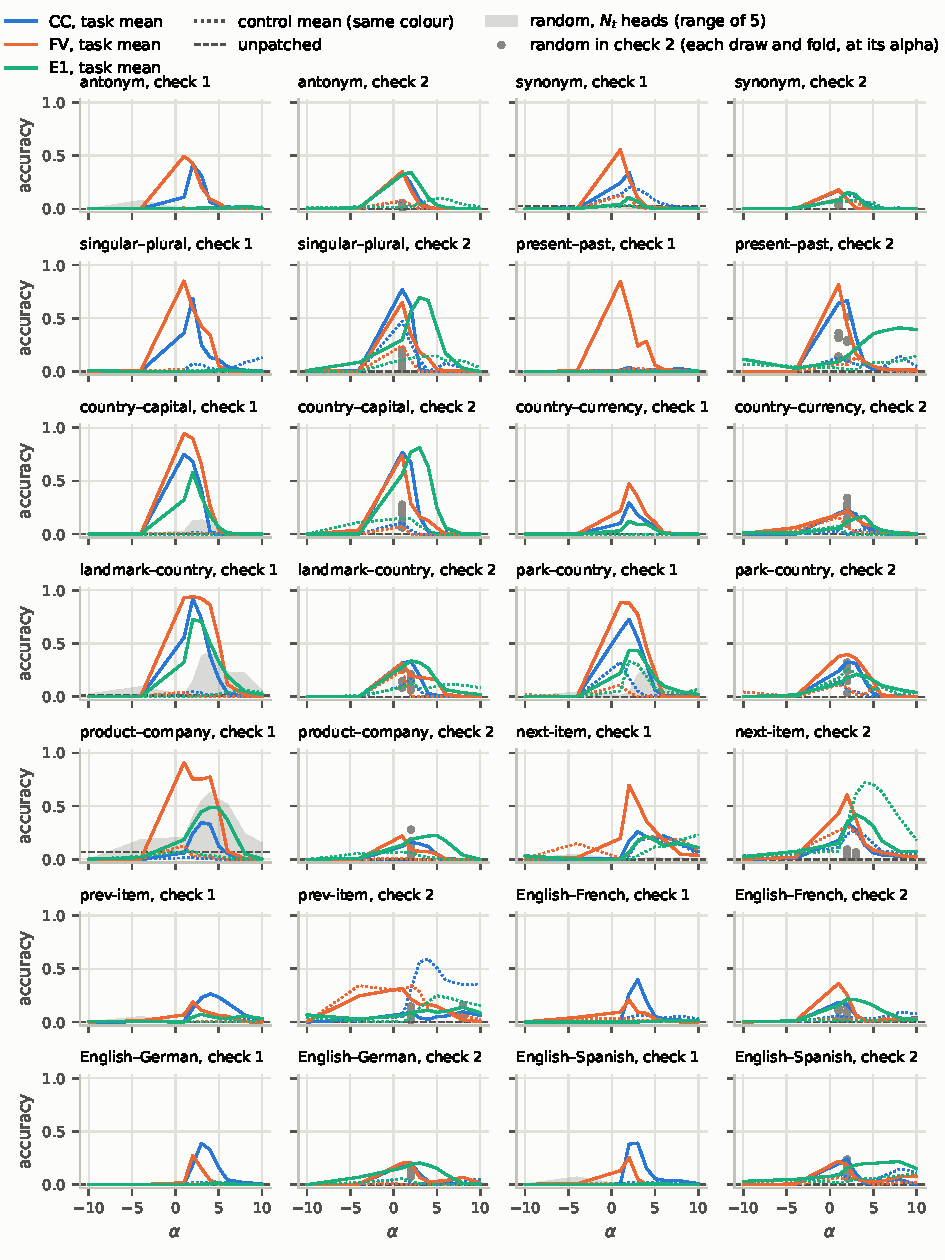
\includegraphics[width=\textwidth]{figures/heldout_curves_nt}
\caption{E4, accuracy against $\alpha$, mean of the two folds, sets of $N_t$ heads: CC, FV-$N_t$ and E1, task means (solid) and control mean (dotted, same colour). Grey band: range of the five random draws (first check); grey points: random draws in the second check, where they are run only at the cross-fitted $\alpha$ (each draw and fold).}
\label{fig:e4-curves-nt}
\end{figure}

\subsection{E4b: More wordings, and wordings held out}
\label{sec:e4b}

\paragraph{Question.} The five templates of \citet{yang2026shared} are few, and E3's word lists and
heads were chosen on all of them, so nothing has been tested on a wording that was not used
to choose. Two questions. First, a head may carry the task but decode a list word only under
some wordings; then more wordings should find more of the heads that carry the task, as
pooling the five templates did in Sec.~\ref{sec:words} (0.18 to 0.45, with five times the prompts of the
best template). Second, if a set holds the task's
representation and not the words of particular instructions, its heads should come up, and its
patch should work, under wordings never used to choose it, including wordings that do not
contain the task's name.

\paragraph{New wordings.} For each task, 30 new instruction templates, in six cells of five:
three forms $\times$ whether the instruction names the task.
\begin{itemize}
  \item Forms: \emph{cloze} (``The opposite of \{x\} is''), \emph{question--answer} (an
    instruction, then \verb|Q: {x}\nA:|, as Yang's templates B--E), and
    \emph{label} (two labels, one before the input and one after it, \verb|Word: {x}\nOpposite:|).
  \item Task named: the instruction contains a word of the task's term list of \citet{yang2026shared} or
    the task's name (antonym, capital, French, \ldots). Not named: it contains none of them
    and describes the task otherwise (``the word whose meaning is furthest from'', ``the city where
    the government of \{x\} sits'', ``this word as a person in Lyon would say it''). Presence is
    checked by script on the lowercased words.
\end{itemize}
They are written by an LLM (GPT-5.5, with one fixed prompt per cell that gives the task's
description and two of Yang's templates as examples, not the items), checked by script for the
cell's conditions and by hand for correctness and ambiguity (one pass by the author), and the
first five per cell that pass are kept. A cell that cannot be filled (the not-named translation
cells may be hard) is reported with the number kept. Yang's five templates are kept as they are.

\paragraph{Behaviour (E0 on the new wordings).} Every new template is run on every item (at
most 500 per task, the same items for all templates), greedy, saved and scored as E0
(Sec.~\ref{sec:evaluation}). Reported: accuracy per template, its spread per task under the flexible and the
first-token score, and the mean accuracy per form and per named / not named. These choose
$P^+$ below, on the choosing half only.

\paragraph{Wording split.} In each of the six cells, three templates are used to choose
(seed~0) and two are held out: 18 new templates to choose and 12 held out per task, the held-out
twelve two per cell. Yang's five templates are always among those used to choose, so that the
sets of E4 are the condition $m = 5$ below. Held-out wordings are never used to choose words,
heads, rankings or $\alpha$. The wording split is crossed with the item split: words and heads
are chosen on the choosing half under the chosen wordings, and every test is on the testing
half.

\paragraph{Conditions: number of wordings.} $m \in \{1, 5, 11, 23\}$ wordings to choose words
and heads, nested: $m = 1$, the most accurate of Yang's templates on the choosing half (the
``best template'' of Sec.~\ref{sec:words}); $m = 5$, Yang's five; $m = 11$, Yang's five and one new template
from each cell, three draws (seeds 0--2); $m = 23$, Yang's five and all 18 new ones. The number
of prompts is held fixed so that $m$ changes how varied the prompts are, not how many: each
condition uses $T_t$ correct prompts in all, where $T_t$ is the number of correct prompts of the
$m = 1$ template on the choosing half, capped at 500, split evenly over the $m$ templates (the
first correct prompts of each; a shortfall in one template is reported, not filled from
another). The $m = 5$ condition is therefore not the CC set of E4, which takes up to 100
prompts from each of the five templates: the two are the same set only where $T_t = 500$
(antonym, synonym and the three translations), and on the other tasks the $m = 5$ condition
has fewer prompts per template (about 15 to 75). The CC set of E4 is reported beside the
conditions as a reference point (five templates, up to 100 prompts each), not as one of them.
Secondary, at $m = 23$: 100 prompts per template, to see
whether more prompts add to more wordings.

\paragraph{Head sets.} For each $m$, the CC rule of E4 unchanged: word shares, task and
common words, and Definition~\ref{def:lth} on the pooled prompts of the $m$ templates; the other 13
tasks' shares for the contrast are computed under the same $m$. Secondary: \textbf{E1-pooled},
Yang's term list with Definition~\ref{def:lth} on the same pooled prompts, at $m = 5$ and $m = 23$, to see
whether more wordings help the hand-written lists. For the $m = 5$ condition, five random sets
with the same number of heads in each layer are drawn as in E4 (seeds 0--4), since the set
differs from E4's.

\paragraph{Tests.}
\begin{enumerate}
  \item \textbf{Number of wordings}: both checks of E4 for every set, with the same five means
    (Yang's templates, choosing half) and the same items, so that only the heads differ;
    cross-fitted $\alpha$ by condition ($m$). The CC set of E4 is shown beside the four
    conditions. Measures beside the effect: set size; overlap
    (Jaccard) between the three $m = 11$ draws and between consecutive $m$; overlap of the
    word lists.
  \item \textbf{Reach on held-out wordings}: for the E1 set, CC ($m = 5$) and CC ($m = 23$),
    the match rate of the set's heads (its own word list, Definition~\ref{def:lth}'s per-prompt test) on the
    correct prompts of each held-out template on the choosing half, against five random sets
    with the same number of heads in each layer as the set (drawn as in E4); separately for
    named and not-named templates, with the copy share (Sec.~\ref{sec:measures}) on each.
  \item \textbf{Held-out means}: check~1 on the same three sets, patched with the means of the
    12 held-out templates (each from its correct prompts on the choosing half) instead of
    Yang's five.
  \item \textbf{Held-out failures}: a second check on wordings, not shots. Patched prompts:
    the prompts of each held-out template answered wrongly on the testing half (the first 20
    per template, at most 240), whose unpatched accuracy is 0. Means: Yang's five, choosing
    half. Control: the control mean of E4. This asks whether heads and means taken from the
    chosen wordings repair the wordings on which the model fails, which is the prompt
    sensitivity of \citet{yang2026shared} in its most direct form.
\end{enumerate}
Tests 3 and 4 are run at three values of $\alpha$: the cross-fitted one of the set and 4 and 8.

\paragraph{Hypotheses.} On the cross-fitted effect, mean over the 14 tasks, intervals by the
paired bootstrap of E4.
\begin{description}
  \item[H7 (more wordings).] (a) CC at $m = 5$ has a larger check-1 effect than at $m = 1$
    (interval above 0): pooling templates helps when the number of prompts is the same.
    (b) CC at $m = 23$ has a larger effect than at $m = 5$ (interval above 0). Each part decided
    separately. Expected: (a) holds but with a smaller gain than in Sec.~\ref{sec:words}, where pooling also
    gave five times the prompts; (b) is smaller and may fail, since the union rule (E1b, $k = 1$)
    helped only some tasks. Comparing $m = 5$ with the CC set of E4 shows what the extra prompts
    add at five templates; it is reported, not tested.
  \item[H8 (held-out wordings).] For CC at $m = 5$ and at $m = 23$, each decided separately:
    (a) the match rate on held-out templates is above that of every random draw, on the named
    and on the not-named templates; (b) check~1 with the held-out means is not worse than with
    Yang's means by more than 0.05 (lower end of the interval); (c) on held-out failures, the
    task mean's effect is above the control mean's (interval above 0). Falsified for a set if
    any part fails; parts are reported one by one.
  \item[H9 (copying).] For CC at $m = 5$, the match rate on not-named held-out templates is
    at least half of that on named ones. If it is less, the heads mostly decode list words
    that the instruction contains, and the reach of H8(a) comes from copying.
\end{description}

\paragraph{What the outcomes would mean.} H7(b) and H8 together decide whether ``more
wordings'' improves identification or only enlarges the sets: if (b) holds and the $m = 23$ set
also passes H8 where $m = 5$ fails, the extra wordings found heads that carry the task across
wordings. If H8 holds but H9 fails, the sets work across wordings that name the task and say
little about a representation of the task beyond its name. H8(c) is the result that speaks to
Yang et al.'s main claim: heads and means from some wordings repairing failures of others.

\paragraph{Status.} Only the new wordings exist so far. GPT-5.5 filled all 84 cells (14 tasks $\times$ 6) with five templates each, which passed the script checks, and kept 2 to 5 spares per cell; one call per cell is logged. In the not-named cells the script bans the words that name the answer relation (the term list of \citet{yang2026shared} and the task's name for it); words for the input, such as \emph{country} for country--capital or \emph{landmark}, are allowed. The hand check is pending (\texttt{data/review/e4b\_wordings.md}); E0 on the new wordings, the readings and the patching have not been run.

\paragraph{Cost of E4b.} New-wording E0: 30 templates $\times$ at most 500 items $\times$ 14
tasks $\le$ 210{,}000 replies. Readings (J-head top tokens of every head at the last token): the
23 chosen and 12 held-out templates' correct prompts, at most about 245{,}000 forward passes
without generation. Patching, per task and fold: test~1, 9 new sets (CC at $m = 1$, $m = 5$,
three at $m = 11$, $m = 23$, $m = 23$ with 100 per template, two E1-pooled) $\times$ 12{,}000
$\approx$ 108{,}000; tests~3 and 4, 3 sets $\times$ 3 values of $\alpha$ $\times$ (12 means
$\times$ 100 $+$ 5 means $\times$ 240 $+$ 240 control) $\approx$ 24{,}000; about 132{,}000 per
task and fold, 3.7 million in all.

\subsection{Cost and output}

\paragraph{Cost of E4.} Per task and fold, with $\le 100$ patched items and five task means:
12 main and secondary sets $\times$ 2 checks $\times$ (10 values of $\alpha$ $\times$ 5 means
$+$ 10 $\times$ 1 control) $\times$ 100 $\approx$ 144{,}000 replies; 15 random sets $\times$ 2
checks $\times$ 10 $\times$ 5 $\times$ 100 $\approx$ 150{,}000; in all about 294{,}000 per task
and fold, 8.2 million over 14 tasks and two folds, plus the function-vector scores on each
choosing half. Two cuts keep the hypotheses intact: random sets in check~2 only at the
cross-fitted $\alpha$ (saves about 67{,}000 per task and fold), and the five secondary sets in
fold~1 only (about 60{,}000 in fold~2). Replies can stop at 16 new tokens: the flexible score
reads only the start of the reply, and the longest reference has 15 tokens. E4 and E4b
together: about 11.9 million patched replies before the cuts, 0.2 million new E0 replies and
0.25 million reading passes. If only part can be run, E4 comes first: H4--H6 do not depend on
E4b, while E4b takes its item split, means and control from E4.

\paragraph{Output.} \texttt{results/heldout/fold1/} and \texttt{fold2/}, and for E4b
\texttt{results/heldout/wordings/}: the new templates with their cells and checks, the
wording split, the split (item ids per half), the
word lists and head sets of each fold, the FV scores, accuracies at every $\alpha$ for every set,
mean and check, the cross-fitted and best-$\alpha$ effects, and the bootstrap intervals. Tables:
cross-fitted effect per task and set in check~1 and check~2 (as Table~\ref{tab:words}), and the three
hypothesis comparisons with their intervals; figures: accuracy against $\alpha$ per task for
E1, CC, FV-$N_t$ and the random draws; for E4b, the effect against $m$ per task, and
match rate and effect on held-out templates by form and named / not named.

\section{Plan}\label{sec:plan}
\paragraph{Steps.}
\begin{enumerate}
\item Run E0 and save every reply. Score the saved outputs with the strict and the flexible score (Sec.~\ref{sec:evaluation}).
\item Run E1 under the flexible score, with both causal checks.
\item Run E1b on the rule-style heads ($k=5$, H\ref{h:consensus}), and its exploratory sets for $k=1$ and~3.
\item Run the follow-ups of the union sets (Secs.~\ref{sec:shared}--\ref{sec:noretrieval}) and write them up.
\item Run the equal-size sets (Sec.~\ref{sec:sized}) and write up their results (done).
\item Head sets from decoded words (Sec.~\ref{sec:words}): first check done; held-out items and the second check in E4 (Sec.~\ref{sec:e4}, done).
\item E4b (Sec.~\ref{sec:e4b}): new wordings generated; to do: hand check, E0 on the new wordings, readings and patching.
\end{enumerate}
Reused code and data: the lexical-task-head code of \citet{yang2026shared}; the Head-JLens code and matrices of \citet{merlo2026headjlens}; the task datasets of \citet{todd2024function}.

\paragraph{Limitations.} One model. Rule-based prompts contain task words, so a head may decode them by copying from the prompt; the copy share measures this but does not decide it. Under J-head, some sites rank tokens highly on unrelated prompts as well \citep[Sec.~3.6]{merlo2026headjlens}, so a larger J-head set is not by itself evidence of more task representation; the causal check is needed. $P^{+}$ and the patched items are chosen by the flexible score, which accepts only the reference answer: a prompt answered with another valid answer is counted as wrong.


\paragraph{Deliverables.} Head sets, measures and causal-check curves for every task, style and readout.

\bibliographystyle{plainnat}
\bibliography{references}

\clearpage
\appendix
\section{Effects of the equal-size sets}\label{app:sized}
The causal effects of the equal-size sets of Sec.~\ref{sec:sized}, as the highest accuracy over the nine values of $\alpha$ minus the unpatched accuracy.

\begin{table}[H]
\centering\footnotesize
% Generated by scripts/sized_tex.py from results/.
\begin{tabular}{@{}lcccccccccccc@{}}
\toprule
 & \multicolumn{6}{c}{Rule style} & \multicolumn{6}{c}{Example style} \\
\cmidrule(lr){2-7}\cmidrule(lr){8-13}
 & \multicolumn{2}{c}{$N=5$} & \multicolumn{2}{c}{$N=10$} & \multicolumn{2}{c}{$N=20$} & \multicolumn{2}{c}{$N=5$} & \multicolumn{2}{c}{$N=10$} & \multicolumn{2}{c}{$N=20$} \\
\cmidrule(lr){2-3}\cmidrule(lr){4-5}\cmidrule(lr){6-7}\cmidrule(lr){8-9}\cmidrule(lr){10-11}\cmidrule(lr){12-13}
Task & L & J & L & J & L & J & L & J & L & J & L & J \\
\midrule
antonym & 0.03 & 0.03 & 0.03 & 0.02 & 0.03 & 0.02 & 0.05 & 0.06 & 0.06 & 0.05 & 0.65 & 0.03 \\
synonym & 0.01 & 0.20 & 0.00 & 0.20 & 0.00 & 0.13 & 0.06 & 0.28 & 0.07 & 0.33 & 0.03 & 0.13 \\
singular--plural & 0.12 & 0.02 & 0.00 & 0.02 & 0.02 & 0.03 & 0.01 & 0.38 & 0.04 & 0.43 & 0.39 & 0.90 \\
present--past & 0.00 & 0.00 & 0.00 & 0.00 & 0.00 & 0.01 & 0.00 & 0.87 & 0.02 & 0.92 & -- & -- \\
country--capital & 0.86 & 0.94 & 0.78 & 0.88 & 0.76 & 0.78 & 0.72 & 0.70 & 0.71 & 0.88 & 0.75 & 0.99 \\
country--currency & 0.06 & 0.04 & 0.06 & 0.10 & 0.06 & 0.18 & 0.14 & 0.15 & 0.08 & 0.22 & 0.09 & 0.21 \\
landmark--country & 0.76 & 0.33 & 0.91 & 0.68 & 0.85 & 0.85 & 0.35 & 0.40 & 0.67 & 0.49 & 0.22 & 0.36 \\
park--country & 0.33 & 0.33 & 0.50 & 0.45 & 0.40 & 0.51 & 0.63 & 0.45 & 0.68 & 0.48 & 0.48 & 0.68 \\
product--company & 0.34 & 0.34 & 0.35 & 0.28 & 0.33 & 0.34 & 0.27 & 0.27 & 0.33 & 0.14 & 0.13 & 0.29 \\
next-item & 0.00 & 0.00 & 0.00 & 0.01 & 0.00 & 0.02 & 0.00 & 0.04 & 0.32 & 0.25 & 0.56 & 0.58 \\
prev-item & 0.00 & 0.00 & 0.00 & 0.03 & 0.04 & 0.03 & 0.00 & 0.00 & 0.00 & 0.00 & 0.00 & 0.14 \\
English--French & 0.00 & 0.00 & 0.00 & 0.00 & -- & 0.01 & 0.00 & 0.00 & 0.00 & 0.00 & -- & 0.13 \\
English--German & 0.00 & 0.00 & 0.00 & 0.00 & -- & 0.01 & 0.00 & 0.00 & 0.00 & 0.00 & -- & 0.00 \\
English--Spanish & 0.00 & 0.01 & -- & 0.01 & -- & 0.01 & 0.00 & 0.01 & -- & 0.01 & -- & 0.01 \\
\bottomrule
\end{tabular}

\caption{Equal-size sets, E1 rule, first causal check: causal effect of the $N$ highest-ranked heads with means of their own style, as in Table~\ref{tab:effects-simple}, over the nine values of $\alpha$. L: Logit-head, J: J-head. --: set not formed (fewer than $N$ heads match on any prompt).}
\label{tab:sized-readouts}
\end{table}

\begin{table}[H]
\centering\footnotesize
% Generated by scripts/sized_tex.py from results/.
\begin{tabular}{@{}lcccccccccccc@{}}
\toprule
 & \multicolumn{6}{c}{Rule style} & \multicolumn{6}{c}{Example style} \\
\cmidrule(lr){2-7}\cmidrule(lr){8-13}
 & \multicolumn{2}{c}{$N=5$} & \multicolumn{2}{c}{$N=10$} & \multicolumn{2}{c}{$N=20$} & \multicolumn{2}{c}{$N=5$} & \multicolumn{2}{c}{$N=10$} & \multicolumn{2}{c}{$N=20$} \\
\cmidrule(lr){2-3}\cmidrule(lr){4-5}\cmidrule(lr){6-7}\cmidrule(lr){8-9}\cmidrule(lr){10-11}\cmidrule(lr){12-13}
Task & L & J & L & J & L & J & L & J & L & J & L & J \\
\midrule
antonym & 0.30 & 0.32 & 0.32 & 0.30 & 0.32 & 0.34 & 0.31 & 0.31 & 0.33 & 0.31 & 0.42 & 0.37 \\
synonym & 0.05 & 0.19 & 0.06 & 0.17 & 0.07 & 0.14 & 0.05 & 0.09 & 0.07 & 0.13 & 0.09 & 0.11 \\
singular--plural & 0.58 & 0.59 & 0.45 & 0.68 & 0.58 & 0.73 & 0.69 & 0.76 & 0.81 & 0.86 & 0.79 & 0.87 \\
present--past & 0.34 & 0.36 & 0.43 & 0.45 & 0.44 & 0.51 & 0.61 & 0.80 & 0.56 & 0.83 & -- & -- \\
country--capital & 0.70 & 0.81 & 0.70 & 0.82 & 0.77 & 0.79 & 0.65 & 0.53 & 0.73 & 0.56 & 0.70 & 0.77 \\
country--currency & 0.18 & 0.14 & 0.20 & 0.22 & 0.14 & 0.19 & 0.24 & 0.25 & 0.29 & 0.19 & 0.17 & 0.21 \\
landmark--country & 0.32 & 0.30 & 0.33 & 0.33 & 0.34 & 0.31 & 0.33 & 0.30 & 0.32 & 0.33 & 0.33 & 0.32 \\
park--country & 0.24 & 0.24 & 0.34 & 0.33 & 0.24 & 0.26 & 0.36 & 0.36 & 0.35 & 0.36 & 0.45 & 0.40 \\
product--company & 0.14 & 0.14 & 0.16 & 0.11 & 0.17 & 0.19 & 0.12 & 0.16 & 0.20 & 0.23 & 0.25 & 0.34 \\
next-item & 0.03 & 0.08 & 0.07 & 0.21 & 0.18 & 0.27 & 0.10 & 0.56 & 0.45 & 0.70 & 0.65 & 0.81 \\
prev-item & 0.04 & 0.04 & 0.05 & 0.09 & 0.11 & 0.19 & 0.12 & 0.01 & 0.17 & 0.19 & 0.33 & 0.80 \\
English--French & 0.08 & 0.09 & 0.10 & 0.13 & -- & 0.20 & 0.12 & 0.13 & 0.13 & 0.15 & -- & 0.34 \\
English--German & 0.08 & 0.12 & 0.10 & 0.12 & -- & 0.17 & 0.13 & 0.09 & 0.15 & 0.13 & -- & 0.14 \\
English--Spanish & 0.11 & 0.19 & -- & 0.23 & -- & 0.25 & 0.06 & 0.15 & -- & 0.15 & -- & 0.14 \\
\bottomrule
\end{tabular}

\caption{Equal-size sets, E1 rule, second causal check, as Table~\ref{tab:sized-readouts}. Items: the wrongly answered 1-shot prompts patched; the baseline is 0.}
\label{tab:sized-readouts-wrong}
\end{table}

\begin{table}[H]
\centering\footnotesize
% Generated by scripts/sized_tex.py from results/.
\begin{tabular}{@{}lcccccccccccc@{}}
\toprule
 & \multicolumn{6}{c}{Rule style} & \multicolumn{6}{c}{Example style} \\
\cmidrule(lr){2-7}\cmidrule(lr){8-13}
 & \multicolumn{2}{c}{$N=5$} & \multicolumn{2}{c}{$N=10$} & \multicolumn{2}{c}{$N=20$} & \multicolumn{2}{c}{$N=5$} & \multicolumn{2}{c}{$N=10$} & \multicolumn{2}{c}{$N=20$} \\
\cmidrule(lr){2-3}\cmidrule(lr){4-5}\cmidrule(lr){6-7}\cmidrule(lr){8-9}\cmidrule(lr){10-11}\cmidrule(lr){12-13}
Task & L & J & L & J & L & J & L & J & L & J & L & J \\
\midrule
antonym & 0.00 & 0.00 & 0.00 & 0.00 & 0.00 & 0.00 & 0.00 & 0.00 & 0.00 & 0.00 & 0.19 & 0.00 \\
synonym & 0.01 & 0.13 & 0.01 & 0.05 & 0.00 & 0.03 & 0.05 & 0.03 & 0.05 & 0.07 & 0.01 & 0.05 \\
singular--plural & 0.00 & 0.00 & 0.01 & 0.01 & 0.00 & 0.06 & 0.01 & 0.55 & 0.01 & 0.21 & 0.05 & 0.04 \\
present--past & 0.00 & 0.00 & 0.00 & 0.00 & 0.00 & 0.00 & 0.00 & 0.00 & 0.00 & 0.00 & -- & -- \\
country--capital & 0.02 & 0.04 & 0.01 & 0.02 & 0.01 & 0.01 & 0.02 & 0.03 & 0.02 & 0.03 & 0.01 & 0.02 \\
country--currency & 0.00 & 0.00 & 0.00 & 0.00 & 0.00 & 0.00 & 0.00 & 0.00 & 0.00 & 0.00 & 0.00 & 0.00 \\
landmark--country & 0.00 & 0.01 & 0.01 & 0.01 & 0.00 & 0.13 & 0.01 & 0.00 & 0.00 & 0.01 & 0.00 & 0.00 \\
park--country & 0.03 & 0.03 & 0.56 & 0.38 & 0.28 & 0.59 & 0.57 & 0.29 & 0.36 & 0.19 & 0.21 & 0.48 \\
product--company & 0.02 & 0.02 & 0.03 & 0.02 & 0.02 & 0.01 & 0.02 & 0.02 & 0.01 & 0.00 & 0.01 & 0.03 \\
next-item & 0.00 & 0.00 & 0.00 & 0.01 & 0.00 & 0.08 & 0.00 & 0.01 & 0.00 & 0.22 & 0.08 & 0.52 \\
prev-item & 0.00 & 0.00 & 0.00 & 0.00 & 0.00 & 0.00 & 0.00 & 0.00 & 0.00 & 0.00 & 0.00 & 0.00 \\
English--French & 0.01 & 0.02 & 0.01 & 0.03 & -- & 0.00 & 0.01 & 0.01 & 0.00 & 0.00 & -- & 0.02 \\
English--German & 0.00 & 0.00 & 0.00 & 0.00 & -- & 0.00 & 0.00 & 0.00 & 0.00 & 0.00 & -- & 0.00 \\
English--Spanish & 0.00 & 0.00 & -- & 0.00 & -- & 0.00 & 0.00 & 0.00 & -- & 0.00 & -- & 0.00 \\
\bottomrule
\end{tabular}

\caption{Equal-size sets, E1 rule, first causal check: causal effect of the control mean at the sets of Table~\ref{tab:sized-readouts}.}
\label{tab:sized-readouts-control}
\end{table}

\begin{table}[H]
\centering\footnotesize\setlength{\tabcolsep}{4.5pt}
% Generated by scripts/sized_tex.py from results/.
\begin{tabular}{@{}lcccccccccccc@{}}
\toprule
 & \multicolumn{4}{c}{$N=5$} & \multicolumn{4}{c}{$N=10$} & \multicolumn{4}{c}{$N=20$} \\
\cmidrule(lr){2-5}\cmidrule(lr){6-9}\cmidrule(lr){10-13}
Task & E1 & $k=1$ & $k=3$ & $k=5$ & E1 & $k=1$ & $k=3$ & $k=5$ & E1 & $k=1$ & $k=3$ & $k=5$ \\
\midrule
\multicolumn{13}{@{}l}{\emph{Logit-head}} \\
antonym & 0.03 & 0.01 & 0.02 & 0.02 & 0.03 & 0.02 & 0.03 & 0.02 & 0.03 & 0.02 & 0.03 & 0.01 \\
synonym & 0.01 & 0.00 & 0.02 & 0.01 & 0.00 & 0.00 & 0.00 & -- & 0.00 & $-$0.01 & -- & -- \\
singular--plural & 0.12 & 0.15 & 0.17 & 0.01 & 0.00 & 0.02 & 0.01 & 0.00 & 0.02 & 0.02 & 0.01 & -- \\
present--past & 0.00 & 0.00 & 0.00 & 0.00 & 0.00 & 0.00 & 0.00 & -- & 0.00 & 0.00 & 0.00 & -- \\
country--capital & 0.86 & 0.87 & 0.84 & 0.86 & 0.78 & 0.81 & 0.75 & 0.83 & 0.76 & 0.73 & 0.70 & 0.70 \\
country--currency & 0.06 & 0.04 & 0.06 & 0.06 & 0.06 & 0.06 & 0.06 & 0.06 & 0.06 & 0.06 & 0.06 & 0.05 \\
landmark--country & 0.76 & 0.33 & 0.79 & 0.72 & 0.91 & 0.91 & 0.91 & 0.85 & 0.85 & 0.76 & 0.81 & 0.80 \\
park--country & 0.33 & 0.02 & 0.57 & 0.70 & 0.50 & 0.68 & 0.50 & 0.67 & 0.40 & 0.60 & 0.47 & -- \\
product--company & 0.34 & 0.39 & 0.36 & 0.23 & 0.35 & 0.36 & 0.28 & 0.29 & 0.33 & 0.32 & 0.31 & 0.31 \\
next-item & 0.00 & 0.00 & 0.00 & 0.00 & 0.00 & 0.01 & 0.00 & 0.00 & 0.00 & 0.00 & 0.00 & -- \\
prev-item & 0.00 & 0.00 & 0.00 & 0.00 & 0.00 & 0.00 & 0.00 & 0.00 & 0.04 & 0.03 & 0.02 & -- \\
English--French & 0.00 & 0.00 & 0.00 & 0.00 & 0.00 & 0.00 & 0.00 & 0.00 & -- & -- & -- & -- \\
English--German & 0.00 & 0.00 & 0.00 & 0.00 & 0.00 & 0.00 & 0.00 & 0.00 & -- & 0.00 & -- & -- \\
English--Spanish & 0.00 & 0.00 & 0.00 & 0.00 & -- & 0.00 & -- & -- & -- & -- & -- & -- \\
\multicolumn{13}{@{}l}{\emph{J-head}} \\
antonym & 0.03 & 0.02 & 0.04 & 0.02 & 0.02 & 0.02 & 0.01 & 0.01 & 0.02 & 0.01 & 0.02 & 0.01 \\
synonym & 0.20 & 0.18 & 0.24 & 0.09 & 0.20 & 0.21 & 0.18 & 0.08 & 0.13 & 0.13 & 0.11 & 0.08 \\
singular--plural & 0.02 & 0.12 & 0.01 & 0.00 & 0.02 & 0.02 & 0.01 & 0.01 & 0.03 & 0.03 & 0.01 & -- \\
present--past & 0.00 & 0.01 & 0.00 & -- & 0.00 & 0.01 & 0.00 & -- & 0.01 & 0.32 & -- & -- \\
country--capital & 0.94 & 0.83 & 0.94 & 0.89 & 0.88 & 0.88 & 0.89 & 0.85 & 0.78 & 0.81 & 0.82 & 0.79 \\
country--currency & 0.04 & 0.02 & 0.03 & 0.04 & 0.10 & 0.06 & 0.05 & 0.16 & 0.18 & 0.22 & 0.15 & 0.13 \\
landmark--country & 0.33 & 0.33 & 0.82 & 0.73 & 0.68 & 0.82 & 0.70 & 0.78 & 0.85 & 0.77 & 0.83 & 0.83 \\
park--country & 0.33 & 0.27 & 0.21 & 0.57 & 0.45 & 0.18 & 0.45 & 0.73 & 0.51 & 0.56 & 0.52 & -- \\
product--company & 0.34 & 0.31 & 0.44 & 0.35 & 0.28 & 0.40 & 0.41 & 0.30 & 0.34 & 0.44 & 0.36 & 0.32 \\
next-item & 0.00 & 0.00 & 0.00 & 0.00 & 0.01 & 0.00 & 0.02 & 0.00 & 0.02 & 0.03 & 0.07 & 0.02 \\
prev-item & 0.00 & 0.00 & 0.00 & 0.00 & 0.03 & 0.08 & 0.04 & 0.07 & 0.03 & 0.15 & 0.07 & 0.06 \\
English--French & 0.00 & 0.01 & 0.00 & 0.01 & 0.00 & 0.00 & 0.00 & 0.00 & 0.01 & 0.07 & 0.00 & 0.00 \\
English--German & 0.00 & 0.00 & 0.00 & 0.00 & 0.00 & 0.00 & 0.00 & 0.00 & 0.01 & 0.01 & 0.00 & -- \\
English--Spanish & 0.01 & 0.01 & 0.01 & 0.01 & 0.01 & 0.01 & 0.00 & 0.01 & 0.01 & 0.01 & 0.01 & -- \\
\bottomrule
\end{tabular}

\caption{Equal-size sets, rule style, first causal check: causal effect of the $N$ highest-ranked heads under the rule of E1 and the rules of E1b (at least $k$ of the five templates), as Table~\ref{tab:sized-readouts}.}
\label{tab:sized-rules}
\end{table}

\begin{table}[H]
\centering\footnotesize\setlength{\tabcolsep}{4.5pt}
% Generated by scripts/sized_tex.py from results/.
\begin{tabular}{@{}lcccccccccccc@{}}
\toprule
 & \multicolumn{4}{c}{$N=5$} & \multicolumn{4}{c}{$N=10$} & \multicolumn{4}{c}{$N=20$} \\
\cmidrule(lr){2-5}\cmidrule(lr){6-9}\cmidrule(lr){10-13}
Task & E1 & $k=1$ & $k=3$ & $k=5$ & E1 & $k=1$ & $k=3$ & $k=5$ & E1 & $k=1$ & $k=3$ & $k=5$ \\
\midrule
\multicolumn{13}{@{}l}{\emph{Logit-head}} \\
antonym & 0.30 & 0.27 & 0.26 & 0.28 & 0.32 & 0.28 & 0.29 & 0.29 & 0.32 & 0.30 & 0.31 & 0.25 \\
synonym & 0.05 & 0.04 & 0.04 & 0.06 & 0.06 & 0.04 & 0.06 & -- & 0.07 & 0.08 & -- & -- \\
singular--plural & 0.58 & 0.60 & 0.62 & 0.32 & 0.45 & 0.49 & 0.52 & 0.35 & 0.58 & 0.63 & 0.63 & -- \\
present--past & 0.34 & 0.42 & 0.38 & 0.39 & 0.43 & 0.40 & 0.40 & -- & 0.44 & 0.50 & 0.43 & -- \\
country--capital & 0.70 & 0.81 & 0.73 & 0.72 & 0.70 & 0.81 & 0.75 & 0.70 & 0.77 & 0.79 & 0.81 & 0.74 \\
country--currency & 0.18 & 0.14 & 0.18 & 0.18 & 0.20 & 0.19 & 0.18 & 0.15 & 0.14 & 0.21 & 0.20 & 0.13 \\
landmark--country & 0.32 & 0.29 & 0.32 & 0.33 & 0.33 & 0.33 & 0.33 & 0.34 & 0.34 & 0.34 & 0.34 & 0.33 \\
park--country & 0.24 & 0.19 & 0.33 & 0.38 & 0.34 & 0.37 & 0.34 & 0.32 & 0.24 & 0.26 & 0.25 & -- \\
product--company & 0.14 & 0.12 & 0.15 & 0.12 & 0.16 & 0.15 & 0.11 & 0.17 & 0.17 & 0.22 & 0.17 & 0.16 \\
next-item & 0.03 & 0.04 & 0.04 & 0.04 & 0.07 & 0.08 & 0.06 & 0.07 & 0.18 & 0.07 & 0.09 & -- \\
prev-item & 0.04 & 0.02 & 0.03 & 0.04 & 0.05 & 0.03 & 0.04 & 0.05 & 0.11 & 0.09 & 0.15 & -- \\
English--French & 0.08 & 0.09 & 0.09 & 0.08 & 0.10 & 0.10 & 0.10 & 0.10 & -- & -- & -- & -- \\
English--German & 0.08 & 0.08 & 0.08 & 0.08 & 0.10 & 0.09 & 0.09 & 0.10 & -- & 0.12 & -- & -- \\
English--Spanish & 0.11 & 0.14 & 0.11 & 0.11 & -- & 0.15 & -- & -- & -- & -- & -- & -- \\
\multicolumn{13}{@{}l}{\emph{J-head}} \\
antonym & 0.32 & 0.30 & 0.27 & 0.27 & 0.30 & 0.35 & 0.31 & 0.29 & 0.34 & 0.35 & 0.32 & 0.27 \\
synonym & 0.19 & 0.17 & 0.17 & 0.13 & 0.17 & 0.18 & 0.17 & 0.12 & 0.14 & 0.14 & 0.13 & 0.12 \\
singular--plural & 0.59 & 0.58 & 0.54 & 0.14 & 0.68 & 0.75 & 0.55 & 0.38 & 0.73 & 0.76 & 0.74 & -- \\
present--past & 0.36 & 0.37 & 0.28 & -- & 0.45 & 0.50 & 0.49 & -- & 0.51 & 0.72 & -- & -- \\
country--capital & 0.81 & 0.82 & 0.81 & 0.62 & 0.82 & 0.82 & 0.82 & 0.83 & 0.79 & 0.80 & 0.78 & 0.84 \\
country--currency & 0.14 & 0.13 & 0.14 & 0.14 & 0.22 & 0.17 & 0.14 & 0.19 & 0.19 & 0.23 & 0.19 & 0.20 \\
landmark--country & 0.30 & 0.29 & 0.33 & 0.33 & 0.33 & 0.33 & 0.33 & 0.34 & 0.31 & 0.32 & 0.31 & 0.31 \\
park--country & 0.24 & 0.25 & 0.28 & 0.33 & 0.33 & 0.28 & 0.33 & 0.32 & 0.26 & 0.36 & 0.27 & -- \\
product--company & 0.14 & 0.17 & 0.17 & 0.13 & 0.11 & 0.19 & 0.15 & 0.13 & 0.19 & 0.28 & 0.19 & 0.22 \\
next-item & 0.08 & 0.06 & 0.04 & 0.04 & 0.21 & 0.08 & 0.19 & 0.06 & 0.27 & 0.39 & 0.39 & 0.21 \\
prev-item & 0.04 & 0.04 & 0.04 & 0.04 & 0.09 & 0.08 & 0.04 & 0.06 & 0.19 & 0.09 & 0.10 & 0.09 \\
English--French & 0.09 & 0.13 & 0.09 & 0.15 & 0.13 & 0.14 & 0.10 & 0.10 & 0.20 & 0.19 & 0.16 & 0.13 \\
English--German & 0.12 & 0.15 & 0.11 & 0.12 & 0.12 & 0.14 & 0.11 & 0.11 & 0.17 & 0.19 & 0.15 & -- \\
English--Spanish & 0.19 & 0.19 & 0.19 & 0.19 & 0.23 & 0.16 & 0.21 & 0.18 & 0.25 & 0.22 & 0.25 & -- \\
\bottomrule
\end{tabular}

\caption{Equal-size sets, rule style, second causal check, as Table~\ref{tab:sized-rules}. The baseline is 0.}
\label{tab:sized-rules-wrong}
\end{table}

\clearpage
\section{E4: accuracy curves at 20 and 40 heads}\label{app:e4}
\begin{figure}[H]
\centering
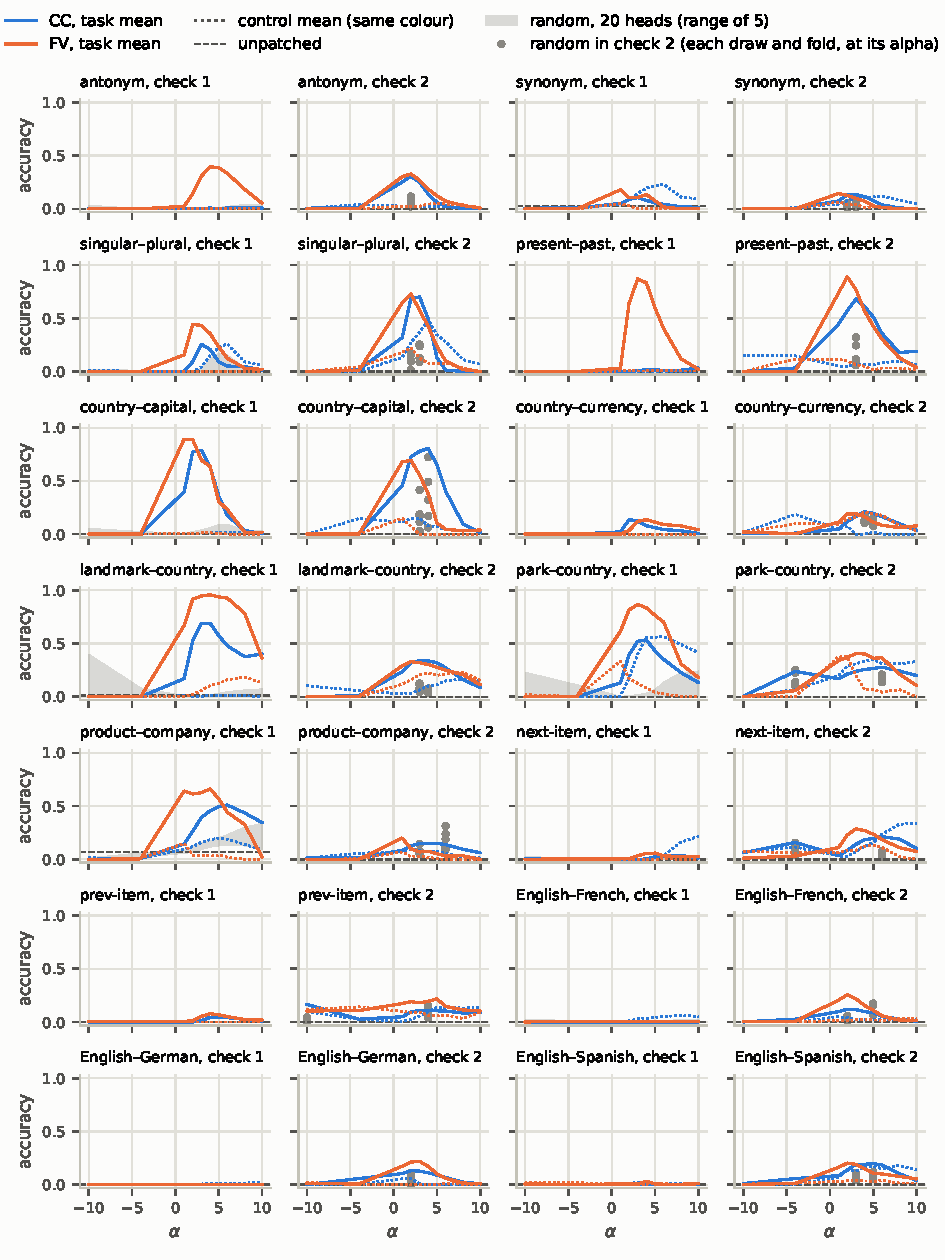
\includegraphics[width=\textwidth]{figures/heldout_curves_20}
\caption{E4, accuracy against $\alpha$, sets of 20 heads (CC-20, FV-20, Random-20), as Figure~\ref{fig:e4-curves-nt}; E1 as there.}
\label{fig:e4-curves-20}
\end{figure}
\begin{figure}[H]
\centering
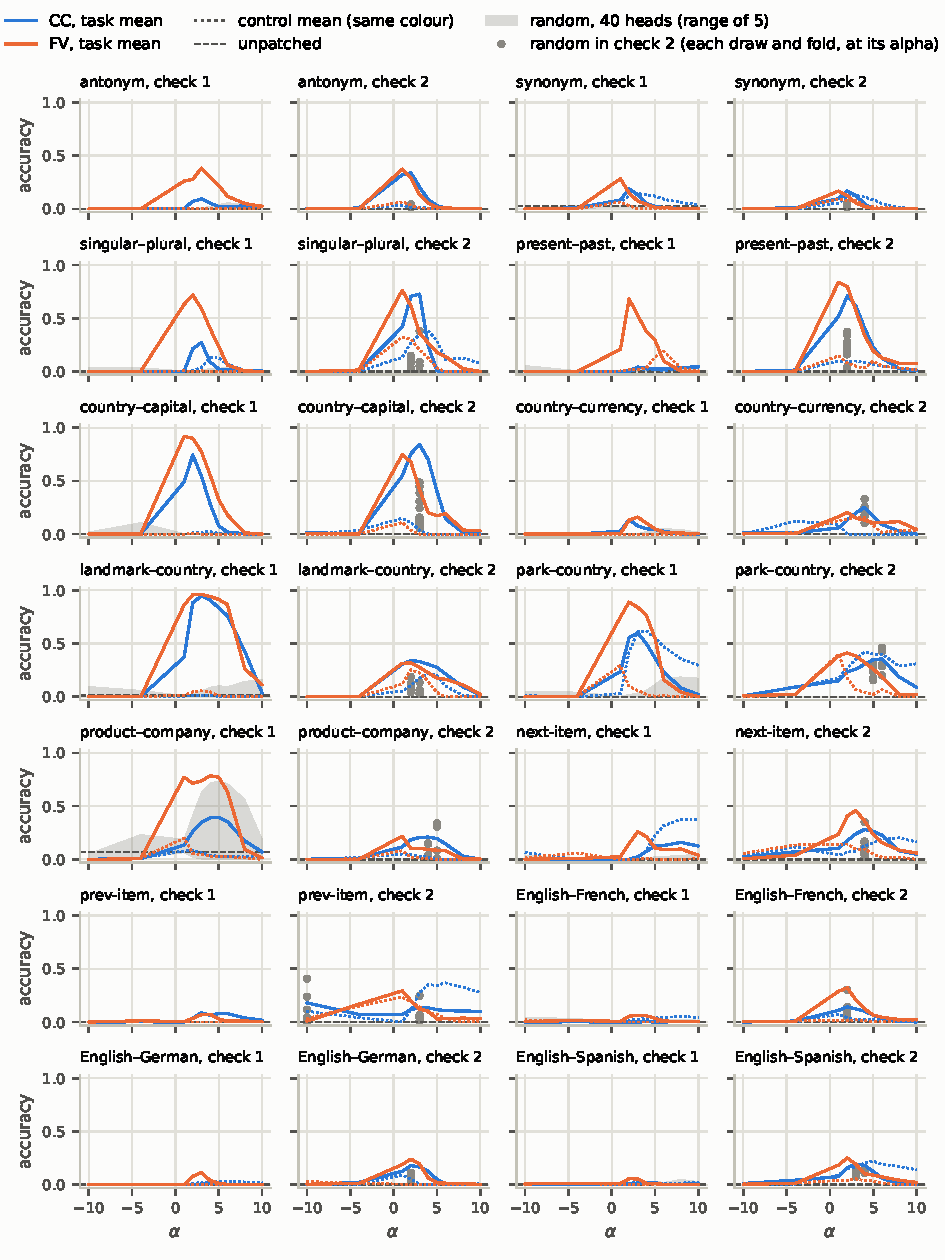
\includegraphics[width=\textwidth]{figures/heldout_curves_40}
\caption{E4, accuracy against $\alpha$, sets of 40 heads, as Figure~\ref{fig:e4-curves-20}.}
\label{fig:e4-curves-40}
\end{figure}

\clearpage
% Generated by scripts/appendix_simple_tex.py from Yang et al.'s term lists and templates.
\section{Term lists}\label{app:terms-simple}
The term list $V_t$ of each task, as in the file of \citet[App.~A.2.1]{yang2026shared}, and the single tokens it expands to, as in their code: each term is tried as written, with a leading space, in upper, capitalised and lower case, and after a \texttt{.}, \texttt{\_} or \texttt{-}; every variant that is one token of the Llama-3.1 tokenizer is kept. A head matches a prompt when one of its ten highest-scoring tokens is one of these (Definition~\ref{def:lth}). Terms marked $\dagger$ have no variant that is one token, so they never match. \textvisiblespace: leading space; U+: a character outside Latin script, by its code point.

\begin{center}\footnotesize\frenchspacing
\begin{tabular}{@{}l>{\raggedright}p{0.28\textwidth}>{\raggedright\arraybackslash}p{0.49\textwidth}@{}}
\toprule
Task & Terms & Tokens \\
\midrule
antonym & opposite, reverse, antonym$^\dagger$, opposing, \textrm{U+53CD} & \texttt{\textvisiblespace{}opposing}, \texttt{\textvisiblespace{}opposite}, \texttt{\textvisiblespace{}reverse}, \texttt{.reverse}, \texttt{Reverse}, \texttt{\_reverse}, \texttt{reverse}, \texttt{\textrm{U+53CD}} (8) \\[2pt]
synonym & synonym, equivalent, alike, similar, analogous, interchangeable, \textrm{U+76F8} \textrm{U+8FD1}$^\dagger$, \textrm{U+8FD1} \textrm{U+4E49} \textrm{U+8BCD}$^\dagger$ & \texttt{\textvisiblespace{}alike}, \texttt{\textvisiblespace{}analogous}, \texttt{\textvisiblespace{}equivalent}, \texttt{Equivalent}, \texttt{\textvisiblespace{}interchangeable}, \texttt{\textvisiblespace{}similar}, \texttt{Similar}, \texttt{similar}, \texttt{\textvisiblespace{}synonym} (9) \\[2pt]
singular--plural & plural, multiple, \textrm{U+591A}, Multiplicity, \_multiple, ones & \texttt{\textvisiblespace{}multiple}, \texttt{Multiple}, \texttt{\_multiple}, \texttt{multiple}, \texttt{Multiplicity}, \texttt{\textvisiblespace{}ones}, \texttt{.ones}, \texttt{ONES}, \texttt{ones}, \texttt{\textvisiblespace{}plural}, \texttt{\_plural}, \texttt{plural}, \texttt{\textvisiblespace{}\textrm{U+591A}}, \texttt{\textrm{U+591A}} (14) \\[2pt]
present--past & past, previously, Earlier, previouslyhistorical$^\dagger$, previously, Preceding$^\dagger$ & \texttt{\textvisiblespace{}Earlier}, \texttt{Earlier}, \texttt{\textvisiblespace{}past}, \texttt{Past}, \texttt{\_past}, \texttt{past}, \texttt{\textvisiblespace{}previously}, \texttt{Previously} (8) \\[2pt]
country--capital & city, cities, capital, capitals & \texttt{\textvisiblespace{}capital}, \texttt{-capital}, \texttt{Capital}, \texttt{capital}, \texttt{\textvisiblespace{}capitals}, \texttt{\textvisiblespace{}cities}, \texttt{Cities}, \texttt{cities}, \texttt{\textvisiblespace{}city}, \texttt{-city}, \texttt{.city}, \texttt{City}, \texttt{\_city}, \texttt{city} (14) \\[2pt]
country--currency & currency, currencies, money & \texttt{\textvisiblespace{}currencies}, \texttt{\textvisiblespace{}currency}, \texttt{.currency}, \texttt{Currency}, \texttt{\_currency}, \texttt{currency}, \texttt{\textvisiblespace{}money}, \texttt{-money}, \texttt{.money}, \texttt{Money}, \texttt{\_money}, \texttt{money} (12) \\[2pt]
landmark--country & countries, country, \textrm{U+56FD} \textrm{U+5BB6}, nation & \texttt{\textvisiblespace{}countries}, \texttt{Countries}, \texttt{\_countries}, \texttt{countries}, \texttt{\textvisiblespace{}country}, \texttt{-country}, \texttt{.country}, \texttt{Country}, \texttt{\_country}, \texttt{country}, \texttt{\textvisiblespace{}nation}, \texttt{Nation}, \texttt{nation}, \texttt{\textvisiblespace{}\textrm{U+56FD} \textrm{U+5BB6}}, \texttt{\textrm{U+56FD} \textrm{U+5BB6}} (15) \\[2pt]
park--country & countries, country, \textrm{U+56FD} \textrm{U+5BB6} & \texttt{\textvisiblespace{}countries}, \texttt{Countries}, \texttt{\_countries}, \texttt{countries}, \texttt{\textvisiblespace{}country}, \texttt{-country}, \texttt{.country}, \texttt{Country}, \texttt{\_country}, \texttt{country}, \texttt{\textvisiblespace{}\textrm{U+56FD} \textrm{U+5BB6}}, \texttt{\textrm{U+56FD} \textrm{U+5BB6}} (12) \\[2pt]
product--company & company, companies, firm, firms, manufacturers, manufacturerpublisher$^\dagger$, corporations, corporation, organisations, organisation, institution, institutions & \texttt{\textvisiblespace{}companies}, \texttt{Companies}, \texttt{companies}, \texttt{\textvisiblespace{}company}, \texttt{-company}, \texttt{.company}, \texttt{Company}, \texttt{\_company}, \texttt{company}, \texttt{\textvisiblespace{}corporation}, \texttt{\textvisiblespace{}corporations}, \texttt{\textvisiblespace{}firm}, \texttt{firm}, \texttt{\textvisiblespace{}firms}, \texttt{\textvisiblespace{}institution}, \texttt{institution}, \texttt{\textvisiblespace{}institutions}, \texttt{\textvisiblespace{}manufacturers}, \texttt{\textvisiblespace{}organisation}, \texttt{organisation}, \texttt{\textvisiblespace{}organisations} (21) \\[2pt]
next-item & next, following, after, Following, \textrm{U+63A5} \textrm{U+7740}, -next, .next & \texttt{\textvisiblespace{}after}, \texttt{-after}, \texttt{.after}, \texttt{After}, \texttt{\_after}, \texttt{after}, \texttt{\textvisiblespace{}Following}, \texttt{\textvisiblespace{}following}, \texttt{Following}, \texttt{following}, \texttt{\textvisiblespace{}next}, \texttt{-next}, \texttt{.next}, \texttt{NEXT}, \texttt{Next}, \texttt{\_next}, \texttt{next}, \texttt{\textrm{U+63A5} \textrm{U+7740}} (18) \\[2pt]
prev-item & previous, before, previously, last, earlier, \_previous & \texttt{\textvisiblespace{}before}, \texttt{-before}, \texttt{.before}, \texttt{Before}, \texttt{\_before}, \texttt{before}, \texttt{\textvisiblespace{}earlier}, \texttt{Earlier}, \texttt{\textvisiblespace{}last}, \texttt{-last}, \texttt{.last}, \texttt{LAST}, \texttt{Last}, \texttt{\_last}, \texttt{last}, \texttt{\textvisiblespace{}previous}, \texttt{.previous}, \texttt{Previous}, \texttt{\_previous}, \texttt{previous}, \texttt{\textvisiblespace{}previously}, \texttt{Previously} (22) \\[2pt]
English--French & french, \textrm{U+6CD5} \textrm{U+8BED}$^\dagger$, Français$^\dagger$ & \texttt{\textvisiblespace{}french}, \texttt{French} (2) \\[2pt]
English--German & german, \textrm{U+5FB7} \textrm{U+8BED}$^\dagger$, Deutsch & \texttt{\textvisiblespace{}Deutsch}, \texttt{\textvisiblespace{}german}, \texttt{German} (3) \\[2pt]
English--Spanish & spanish, \textrm{U+897F} \textrm{U+73ED} \textrm{U+7259} \textrm{U+8BED}$^\dagger$, Español$^\dagger$ & \texttt{\textvisiblespace{}spanish}, \texttt{Spanish} (2) \\[2pt]
\bottomrule
\end{tabular}
\end{center}

\section{Instruction templates}\label{app:templates-simple}
\begin{sloppypar}The five instruction templates of each task, the rule-style prompts of \citet[App.~A.3.1]{yang2026shared} (templates A--E, the first five of their instruction file). \texttt{\{input\}} is replaced by the item and the prompt ends after the last character shown; $\hookleftarrow$: newline. $^\ast$: the template whose prompts identify the rule-style heads of E1, the most accurate under the flexible score (Sec.~\ref{sec:e1}); E1b uses all five. Example-style prompts have no instruction: $n$ items of the dataset as ``\texttt{\textvisiblespace\{input\}:\textvisiblespace\{output\};}'', followed by the query as ``\texttt{\textvisiblespace\{input\}:}'' (\textvisiblespace: space), for instance the 1-shot antonym prompt ``\texttt{\textvisiblespace{}bondage:\textvisiblespace{}freedom;\textvisiblespace{}flawed:}''; the zero-shot prompt is the query alone.\end{sloppypar}

{\footnotesize\frenchspacing
\begin{longtable}{@{}ll>{\raggedright\arraybackslash}p{0.74\textwidth}@{}}
\toprule
Task & & Template \\
\midrule
\endhead
\bottomrule
\endfoot
antonym & A & \texttt{The antonym of \{input\} is} \\
 & B & \texttt{Output the antonym of the word in the question. Q: \{input\}$\hookleftarrow$A:} \\
 & C$^\ast$ & \texttt{Give me the antonym of the following word. Q: \{input\}$\hookleftarrow$A:} \\
 & D & \texttt{What word is the opposite of the word in the question? Q: \{input\}$\hookleftarrow$A:} \\
 & E & \texttt{Give an antonym for the following word: Q: \{input\}$\hookleftarrow$A:} \\[3pt]
synonym & A & \texttt{A synonym for \{input\} is} \\
 & B & \texttt{Output the synonym of the question. Q: \{input\}$\hookleftarrow$A:} \\
 & C & \texttt{Task: Synonym Q: \{input\}$\hookleftarrow$A:} \\
 & D & \texttt{Word to synonym Q: \{input\}$\hookleftarrow$A:} \\
 & E$^\ast$ & \texttt{What is the synonym? Q: \{input\}$\hookleftarrow$A:} \\[3pt]
singular--plural & A & \texttt{The plural form of \{input\} is} \\
 & B$^\ast$ & \texttt{What is the plural of the following word? Q: \{input\}$\hookleftarrow$A:} \\
 & C & \texttt{Task: Singlular to Plural Q: \{input\}$\hookleftarrow$A:} \\
 & D & \texttt{Could you please tell me what is the plural word? Q: \{input\}$\hookleftarrow$A:} \\
 & E & \texttt{Output the plural word from the singular Q: \{input\}$\hookleftarrow$A:} \\[3pt]
present--past & A & \texttt{The past tense of \{input\} is} \\
 & B & \texttt{Write the word in its past tense form. Q: \{input\}$\hookleftarrow$A:} \\
 & C$^\ast$ & \texttt{What is the past tense of the following verb? Q: \{input\}$\hookleftarrow$A:} \\
 & D & \texttt{Give me the past tense of \textquotesingle{}Q\textquotesingle{} Q: \{input\}$\hookleftarrow$A:} \\
 & E & \texttt{I wonder what the past tense of this English word is. Can you tell me? Q: \{input\}$\hookleftarrow$A:} \\[3pt]
country--capital & A & \texttt{The capital city of \{input\} is} \\
 & B & \texttt{What is the capital of the country? Q: \{input\}$\hookleftarrow$A:} \\
 & C & \texttt{Country -> Capital Q: \{input\}$\hookleftarrow$A:} \\
 & D$^\ast$ & \texttt{Task: given the country, answer the capital of the country. Q: \{input\}$\hookleftarrow$A:} \\
 & E & \texttt{What capital city does this country have? Q: \{input\}$\hookleftarrow$A:} \\[3pt]
country--currency & A$^\ast$ & \texttt{The currency of \{input\} is the} \\
 & B & \texttt{What is the currency used by the country? Q: \{input\}$\hookleftarrow$A:} \\
 & C & \texttt{Country -> Currency Q: \{input\}$\hookleftarrow$A:} \\
 & D & \texttt{Task: given the country, answer with the currency of the country. Q: \{input\}$\hookleftarrow$A:} \\
 & E & \texttt{What currency does this country use? Q: \{input\}$\hookleftarrow$A:} \\[3pt]
landmark--country & A & \texttt{The country where \{input\} is located is} \\
 & B$^\ast$ & \texttt{Which country does this landmark belong to? Q: \{input\}$\hookleftarrow$A:} \\
 & C & \texttt{Return the country that this landmark is in. Q: \{input\}$\hookleftarrow$A:} \\
 & D & \texttt{Help me find the country that the mentioned landmark is located in. Q: \{input\}$\hookleftarrow$A:} \\
 & E & \texttt{Landmark -> Country. Q: \{input\}$\hookleftarrow$A:} \\[3pt]
park--country & A & \texttt{The country where \{input\} is located is} \\
 & B & \texttt{What is the country of the park? Q: \{input\}$\hookleftarrow$A:} \\
 & C & \texttt{Which nation does the park belong to? Q: \{input\}$\hookleftarrow$A:} \\
 & D & \texttt{Park -> Country Q: \{input\}$\hookleftarrow$A:} \\
 & E$^\ast$ & \texttt{Which country is this place located in? Q: \{input\}$\hookleftarrow$A:} \\[3pt]
product--company & A & \texttt{The company that produces \{input\} is} \\
 & B & \texttt{Which company is the product from? Q: \{input\}$\hookleftarrow$A:} \\
 & C & \texttt{Which company makes the given product? Q: \{input\}$\hookleftarrow$A:} \\
 & D & \texttt{Task definition: given a product, which company makes it? Q: \{input\}$\hookleftarrow$A:} \\
 & E$^\ast$ & \texttt{Product -> Company owning it Q: \{input\}$\hookleftarrow$A:} \\[3pt]
next-item & A$^\ast$ & \texttt{The next item after \{input\} is} \\
 & B & \texttt{What is the next item in the sequence? Q: \{input\}$\hookleftarrow$A:} \\
 & C & \texttt{Given the current item, what is the next item in the sequence? Q: \{input\}$\hookleftarrow$A:} \\
 & D & \texttt{Find the next item. Q: \{input\}$\hookleftarrow$A:} \\
 & E & \texttt{Return the item that is sequentially next of the given input Q: \{input\}$\hookleftarrow$A:} \\[3pt]
prev-item & A & \texttt{The previous item before \{input\} is} \\
 & B$^\ast$ & \texttt{Given a number, letter, or month, return the previous item in the sequence. Q: \{input\}$\hookleftarrow$A:} \\
 & C & \texttt{Return the previous item in the sequence. Q: \{input\}$\hookleftarrow$A:} \\
 & D & \texttt{Instruction: given the current item, what is the previous one? Q: \{input\}$\hookleftarrow$A:} \\
 & E & \texttt{You are given an item in the squence, what is the previous item? Q: \{input\}$\hookleftarrow$A:} \\[3pt]
English--French & A & \texttt{The French translation of \{input\} is} \\
 & B & \texttt{Translate English to French: Q: \{input\}$\hookleftarrow$A:} \\
 & C & \texttt{What is the French translation of the following English sentence? Q: \{input\}$\hookleftarrow$A:} \\
 & D$^\ast$ & \texttt{Given an English word, can you translate it into French? Q: \{input\}$\hookleftarrow$A:} \\
 & E & \texttt{Write the translation of the following sentence in French. Q: \{input\}$\hookleftarrow$A:} \\[3pt]
English--German & A & \texttt{The German translation of \{input\} is} \\
 & B$^\ast$ & \texttt{Translate the following English word to German. Q: \{input\}$\hookleftarrow$A:} \\
 & C & \texttt{What is the German translation of the following English sentence? Q: \{input\}$\hookleftarrow$A:} \\
 & D & \texttt{Given an English word, can you translate it into German? Q: \{input\}$\hookleftarrow$A:} \\
 & E & \texttt{Write the translation of the following sentence in German. Q: \{input\}$\hookleftarrow$A:} \\[3pt]
English--Spanish & A & \texttt{The Spanish translation of \{input\} is} \\
 & B & \texttt{Translate the following English sentences to Spanish. Q: \{input\}$\hookleftarrow$A:} \\
 & C$^\ast$ & \texttt{Translate the following English word to Spanish. Q: \{input\}$\hookleftarrow$A:} \\
 & D & \texttt{What is the translation of the word in Spanish? Q: \{input\}$\hookleftarrow$A:} \\
 & E & \texttt{English to Spanish translation: Q: \{input\}$\hookleftarrow$A:} \\[3pt]
\end{longtable}
}


\clearpage
\section*{Decision log}\label{app:decisions}
\addcontentsline{toc}{section}{Decision log}
\begin{description}
\item[2026-10-27] Scope: test the lexical-task-head method of \citet{yang2026shared} on complex tasks and compare the per-head logit lens with Head-JLens. New title.
\item[2026-10-27] Tasks: the 14 simple tasks shared by \citet{yang2026shared} and \citet{davidson2025different}; the five tasks of \citet{fu2026rules}.
\item[2026-10-27] No main condition: rule-based and example-based prompts are treated alike (replacing the earlier choice of rules as main and examples as secondary).
\item[2026-10-27] Method: lexical task heads, with Logit-head and J-head readouts. Function vectors, function-specific heads and the hidden-state difference between prompts are not used for now.
\item[2026-10-27] Answer format as in the source studies.
\item[2026-10-27] Model: Llama-3.1-8B-Instruct, the main model of \citet{yang2026shared} and the only one with released Head-JLens matrices.
\item[2026-10-27] Accuracy is computed with each source paper's evaluation.
\item[2026-10-27] Prompts on which the model does not answer straight away are left out; other ways of handling them are considered after E0.
\item[2026-10-28] The simple tasks follow the code of \citet{yang2026shared} exactly, except for the J-head readout and the bfloat16 precision of the Head-JLens matrices: five instruction templates (their code and paper do not use the sixth template of their instruction file); heads from one wording per style (5-shot, and the most accurate template); one mean and one patch per source wording; their control mean; their batching. This replaces, for the simple tasks, the pooling of prompts and means over wordings and the use of six templates. E1 was rerun.
\item[2026-10-28] Simple tasks: the padding of each batch is masked. The code of \citet{yang2026shared} passes no attention mask, so the model attends to the padding, which their paper does not describe. E1 was rerun.
\item[2026-10-28] Simple tasks: a second causal check with the setting of the one causal script of \citet{yang2026shared} (wrongly answered 1-shot prompts patched, no control). It reproduces their Figs.~57 and~62, which the zero-shot procedure of their App.~G.1 does not; both checks are reported.
\item[2026-10-29] Answer evaluation (Sec.~\ref{sec:evaluation}), after \citet{hua2025flaw}: every E0 reply is generated once with longer limits and saved; each is scored with the source evaluation. Head identification and the causal checks keep the strict score until this evaluation is done.
\item[2026-10-29] One generation scheme per group of tasks (Sec.~\ref{sec:evaluation}). Simple tasks: a reply ends at \texttt{;}, at a newline once the reply has begun (a leading newline no longer ends it), at the end of sequence, or at 32 new tokens. Complex tasks: a reply ends at the end of sequence or at 1,024 new tokens, for all five tasks; this replaces the limit of 6,000 in reasoning mode and the stop once the scored answer is complete. The saved outputs are generated again under this scheme. Head identification and the causal checks in reasoning mode were run with the earlier limit of 6,000 tokens and the stop at the answer.
\item[2026-10-29] Heads are read at the last prompt token only; the pre-answer position is dropped, with its results. Which prompts form $P^{+}$ for the complex tasks is decided later. Causal checks: the patch is applied at the last prompt position only, for every task, and every task uses the same 15 values of $\alpha$.
\item[2026-10-30] Simple tasks: a second, flexible score next to the first-token score, which is unchanged: the whole reference at the start of the reply, ignoring case, accents, punctuation and a leading article (Sec.~\ref{sec:evaluation}). It is reported for E0; head identification and the causal checks keep the first-token score.
\item[2026-10-30] Head identification and the causal checks use the flexible score, replacing the first-token score (simple tasks) and the strict score (complex tasks): $P^{+}$ is the prompts answered correctly under it, with no condition that the answer comes first, for both families; the identification wordings, the head sets, the means, the patched items and the controls are chosen by it. Readings and means are taken from the prompts of the saved outputs. In the causal checks the reply is generated as the saved outputs and scored by the flexible score; for the simple tasks this replaces the first token, which is kept as a second score. Both complex-task checks patch 100 items on every task, replacing 10 on Set Game, Operator Function and Tapatan; Operator Function has no second check, as no item is answered wrongly under its original rules prompt. E1 and E2 are rerun.
\item[2026-11-02] E1b: rule-style heads of the simple tasks that meet Definition~\ref{def:lth} under all five instruction templates (H\ref{h:consensus}), patched with both causal checks of E1. Only the rule style and only the simple tasks.
\item[2026-11-02] E1b extended after the result of H\ref{h:consensus}, as an exploratory question without a hypothesis: the heads that meet Definition~\ref{def:lth} under at least one and at least three of the five templates, patched with both checks. E1b now reports the Logit-head and J-head sets only, not the heads found only by J-head, and no copy share.
\item[2026-11-03] The project is split into two documents: \texttt{proposal-simple}, the identification method on the simple tasks (E0 for the simple tasks, E1, E1b), and \texttt{proposal-complex}, the complex tasks (E0 for the complex tasks, E2). Work continues on the simple tasks for now. The readout hypothesis is stated once per document, with its criteria unchanged.
\item[2026-11-03] \texttt{proposal-simple} is reorganised: the replication of \citet{yang2026shared} under both readouts first, then one section per change tried, each with its design followed by its results.
\item[2026-11-03] Head sets of equal size (Sec.~\ref{sec:sized}): the $N\in\{5,10,20\}$ highest-ranked heads under each readout and rule, only among heads that match on at least one prompt; patched with own-style means at nine values of $\alpha$ ($-10$, $-4$, 2, 3, 4, 5, 6, 8, 10) to shorten the run, with the threshold sets compared over the same nine; identical sets are patched once.
\item[2026-11-05] Head sets from decoded words (Sec.~\ref{sec:words}), exploratory: J-head only, rule style, first check only, at $\alpha\in\{1,2,4,8\}$, with the E1 J-head sets compared over the same four values. Word lists from the words all heads decode on $P^{+}$; heads selected on the five templates' prompts pooled.
\item[2026-11-05] Words that heads decode on 1{,}000 WikiText-103 passages are removed from the lists in one variant (CC-pooled-clean), after \citet{davidson2025different}; the 50 most frequent are removed.
\item[2026-11-06] Small head sets ranked by attention to the task words times decode rate (Sec.~\ref{sec:words}), after the pattern of head L16H25.
\item[2026-11-06] E4 (Sec.~\ref{sec:e4}): the designs of Sec.~\ref{sec:words} frozen and tested on held-out items (two folds) with both checks; $\alpha=1$ added to the nine values of Sec.~\ref{sec:sized}; $\alpha$ cross-fitted per task and set. E4b: the $m=5$ condition uses the fixed prompt count $T_t$, with the CC set of E4 as a reference point only.
\item[2026-11-06] E4 is reported as accuracies only (tables and accuracy against $\alpha$); the bootstrap intervals and the decisions on H4--H6 are not computed.
\item[2026-11-06] E4b wordings: in the not-named cells only words that name the answer relation are banned; words for the input are allowed. Generated by GPT-5.5; hand check by the author before use.
\end{description}

\end{document}
